% Desarrollado por Alfredo Sánchez Alberca (asalber@gmail.com)
% ASPECT RATIO FOR YOUTUBE VIDEO
%\documentclass[aspectratio=1610,mathserif,profesionalfont,10pt,dvips,blue,xcolor=table]{beamer}
% ASPECT RATIO FOR PROJECTOR
\documentclass[mathserif,profesionalfont,10pt,dvips,blue,xcolor=table]{beamer} 
% ARTICLE VERSION 
%\documentclass[10pt,a4paper,titlepage]{article} \usepackage{beamerarticle}  

\usepackage{pxfonts}
%\usepackage{lucidaso}
%\usepackage{eulervm}
%\usepackage{mathpazo}
%\renewcommand{\rmdefault}{ibh}
\setbeamersize{text margin left=.5cm, text margin right=.5cm}

%\usetheme[width=0pt,height=20pt,hideallsubsections]{PaloAlto}
%\useoutertheme[width=0pt,height=30pt,hideallsubsections]{sidebar}
\useoutertheme{default}
\useinnertheme[shadow]{rounded}
%\useoutertheme{shadow}
%\usecolortheme[named=red]{structure}
%\useinnertheme[shadow]{rounded}
%\usecolortheme{sidebartab}
%\usecolortheme[overlystylish]{albatross}
%\usecolortheme{crane} 
%\usecolortheme{lily}
\usecolortheme{whale}
\usecolortheme{rose} 
%\setbeamercovered{transparent}

%\beamertemplateshadingbackground{blue!10}{yellow!10} 

% REMOVE NAVIGATIONS SYMBOLS
\setbeamertemplate{navigation symbols}{}

% ITEM BULLETS 
\setbeamertemplate{itemize items}[default]
\setbeamertemplate{enumerate items}[default]

\setbeamertemplate{section in toc}[sections numbered]
\setbeamertemplate{subsection in toc}[subsections numbered]

% HANDOUTS 
% \setbeameroption{show notes}
% \setbeamertemplate{note page}[plain]
% \setbeamerfont{note page}{size=\scriptsize}

% FOOT
\setbeamertemplate{footline}[split]
% \vbox{%
% \tinycolouredline{structure}{\color{white}\textbf{Curso B\'asico de Estad\'istica \hfill%
% \insertshortinstitute\hfill
% \insertframenumber{} / \inserttotalframenumber
% }}%
% }}

\usepackage[utf8]{inputenc}
\usepackage{amsmath}
\usepackage{amsfonts}
\usepackage{amssymb}
\usepackage{array}
\usepackage{multirow}
\usepackage{textcomp}
\usepackage[usenames,dvipsnames]{pstricks}
\usepackage{pst-all,pst-math,pst-plot,pst-infixplot,pst-xkey,pstricks-add}
\usepackage{pst-solides3d}
\usepackage{pst-3dplot}
\usepackage{epsfig} 
\usepackage{graphicx}
\usepackage{colortbl}
\usepackage[colorlinks=true]{hyperref}
\hypersetup{pdfauthor={Alfredo S\'anchez Alberca (asalber@ceu.es)}, pdftitle={Curso b\'asico de C\'alculo}}
\usepackage{breakurl}

\usepackage[spanish]{babel}

%\usepackage{macros}
\definecolor{vollgrau}{rgb}{0.9,0.9,0.9}
\definecolor{colKeys}{rgb}{0,0,1}
\definecolor{colIdentifier}{rgb}{0,0,0}
\definecolor{colComments}{rgb}{1,0.5,0}
\definecolor{colString}{rgb}{0,0.5,0}
\definecolor{coral}{rgb}{1,0.5,0.31}
\definecolor{royalblue1}{rgb}{0.28,0.46,1}

% SPACE BETWEEN PARAGRAFS
\setlength{\parskip}{0.5em}

% THEORMEM ENVIRONMENTS
\theoremstyle{definition}
\newtheorem{definicion}[theorem]{\translation{Definición}}
\newtheorem{teorema}[theorem]{\translation{Teorema}}

% MARGINS FOR ARTICLE
\mode<article>{\usepackage{fullpage}}
\mode<article>{\usepackage[headsep=1cm, top=3cm, bottom=3cm, left=2.54cm, right=2.54cm]{geometry}}

% HEADINGS AND FOOTERS FOR ARTICLE
\mode<article>{
\usepackage{fancyhdr}
\pagestyle{fancy}
\rhead{\sffamily\slshape Curso básico de Cálculo}
\renewcommand{\headrulewidth}{0pt}
%\renewcommand{\floatpagefraction}{.8}
%\renewcommand{\textfraction}{.1} 
}

% SECTION COLOR FOR ARTICLE
\mode<article>{
\usepackage{titlesec}
\titleformat{\section}{\color{royalblue1}\normalfont\Large\bfseries}{\color{royalblue1}\thesection}{1em}{}
\titleformat{\subsection}{\color{royalblue1}\normalfont\large\bfseries}{\color{royalblue1}\thesubsection}{1em}{}
}

% SET COLOR TEXT
\definecolor{gris}{gray}{0.2}
\color{gris}

%========================================================================================
%   DOCUMENT BODY
%========================================================================================

%---------------------------------------------------------------------cover----
\mode<article>{\title{\Huge \ssfamily Curso Básico de Cálculo}}
\mode<presentation>{\title{Curso Básico de Cálculo}}
\author[]{
Eduardo López Ramírez (\url{elopez@ceu.es})\\ 
José Rojo Montijano (\url{jrojo.eps@ceu.es})\\
Anselmo Romero Limón (\url{arlimon@ceu.es})\\
Alfredo Sánchez Alberca (\url{asalber@ceu.es})
}
\mode<presentation>{\institute[USP CEU]{\includegraphics[scale=0.2]{img/logo_uspceu_01}}}
\date{\mode<article>{\includegraphics[scale=0.2]{img/logo_uspceu_01}\\[1cm] }
%Curso 2013-2014\\ 
\textcopyleft Copyleft} 

\begin{document}
\mode<article>{\thispagestyle{empty}\maketitle} 

%---------------------------------------------------------------------slide----
\begin{frame}
\titlepage 
\end{frame}


%---------------------------------------------------------------------slide----
\begin{frame}
\frametitle{Licencia \includegraphics[scale=0.06]{img/cc-logo}}
\mode<article>{\null \vfill \hrule depth 3pt \smallskip}
\input{licencia}
\mode<article>{\smallskip \hrule depth 3pt}
\end{frame} 

\mode<article>{\newpage}

%---------------------------------------------------------------------slide----
\begin{frame}
\mode<presentation>{\frametitle{Contenidos}}
\setlength{\parskip}{0em}
\tableofcontents[hideallsubsections] 
\end{frame}

\section{Geometría analítica}

%---------------------------------------------------------------------slide----
\mode<presentation>{
	\begin{frame}
		\frametitle{Geometría analítica}
		\setlength{\parskip}{0.3em}
		\tableofcontents[sectionstyle=show/hide,hideothersubsections]
	\end{frame}
}

\subsection{Vectores}

%---------------------------------------------------------------------slide----
\begin{frame}
	\frametitle{Escalares}
	Algunos fenómenos de la naturaleza pueden describirse mediante un número referido a una unidad de medida. 
	
	\begin{definicion}[Escalar]
		Un \emph{escalar} es un número que sirve para expresar una magnitud sin dirección.
	\end{definicion}
	\structure{\bfseries Ejemplos} La estatura o el peso de una persona, la temperatura de un gas o el tiempo que tarda un móvil en recorrer una distancia.
	
	Sin embargo, existen otros fenómenos que no pueden describirse adecuadamente mediante un escalar. 
	Si, por ejemplo, un navegante quiere poner rumbo a puerto y sólo conoce de la intensidad del viento, no sabrá qué dirección tomar. 
	La descripción del viento requiere dos elementos, su intensidad y su dirección. 
	
\end{frame}


%---------------------------------------------------------------------slide----
\begin{frame}
	\frametitle{Vectores}
	\begin{definicion}[Vector]
		Un \emph{vector} es un número que sirve para expresar una magnitud y tiene asociada una dirección y un sentido. 
	\end{definicion}
	
	\structure{\bfseries Ejemplos} La velocidad de un móvil o la fuerza que se aplica sobre un objeto.  
	 
	Geométricamente, un vector se representa mediante un segmento orientado, es decir, una flecha.  
	\begin{center}
		\scalebox{0.8}{\begin{pspicture}(0,-2)(11,2)
\rput(2.74,0.37890625){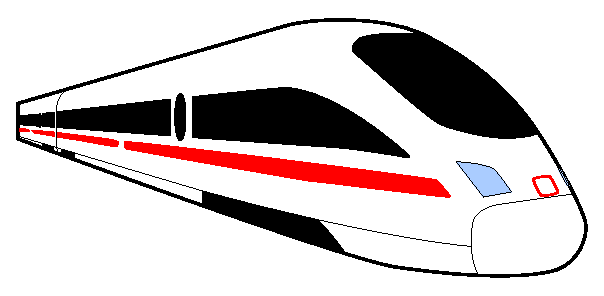
\includegraphics[scale=0.5]{img/geometria_analitica/tren.eps}}
\psline[linewidth=0.08cm,arrowsize=0.05291667cm 2.0,arrowlength=1.4,arrowinset=0.4]{->}(5.72,-0.6610938)(9.34,-1.2610937)
\usefont{T1}{ptm}{m}{n}
\rput(7.5514064,-0.69609374){$\vec{v}$}
\usefont{T1}{ptm}{m}{n}
\rput(10.043282,-1.2360938){dirección}
\psline[linewidth=0.04cm,linecolor=red,tbarsize=0.07055555cm 5.0]{|-|}(5.64,-0.9010937)(9.26,-1.5010937)
\usefont{T1}{ptm}{m}{n}
\rput(7.118906,-1.4560938){magnitud}
\end{pspicture} }
	\end{center}
\end{frame}


% ---------------------------------------------------------------------slide----
\begin{frame}
	\frametitle{Representación de un vector}
	Un segmento orientado puede ubicarse en diferentes lugares dentro de un espacio cartesiano. 
	Sin embargo, con independencia de donde esté situado, si la longitud y la dirección no varían, dicho segmento
	representará siempre el mismo vector.
	
	Esto permite representar todos los vectores con un mismo origen, el origen en sistema de coordenadas cartesianas.
	Así, un vector queda determinado por las \emph{coordenadas} de su extremo final en cualquier espacio euclideo.
	
	\begin{center}
		\scalebox{0.8}{\psset{unit=1,algebraic}
\begin{pspicture}(-4,-2.5)(4,2.5)
\psaxes[ticks=none,labels=none]{<->}(0,0)(-4,-2.5)(4,2.5)
\psline{->}(2,1.5)(4,2.5)
\rput(1.8,1.4){$A$}
\rput(4.2,2.6){$B$}
\psline{->}(-3,0.5)(-1,1.5)
\rput(-3.2,0.4){$C$}
\rput(-0.8,1.6){$D$}
\psline{->}(-1,-2)(1,-1)
\rput(-1.2,-2.1){$E$}
\rput(1.2,-0.9){$F$}
\psline[linecolor=red]{->}(0,0)(2,1)
\rput(1,0.6){$\mathbf{v}$}
\psline[linestyle=dashed, linecolor=gray](2,0)(2,1)(0,1)
\psxTick[ticksize=-3pt 0,labelsep=3pt](2){x}
\psyTick[ticksize=-3pt 0,labelsep=3pt](1){y}
\rput[l](3,0.5){${\mathbf{v}} = (x,y) = \vec{AB}=\vec{CD}=\vec{EF}$}
\end{pspicture}}
	\end{center}
\end{frame} 


% ---------------------------------------------------------------------slide----
\begin{frame}
	\frametitle{Vector a partir de dos puntos}
	Dados dos puntos $P$ y $Q$ de un espacio cartesiano, el vector con origen en $P$ y destino en $Q$ tiene coordenadas $\vec{PQ}=Q-P$.
	
	\structure{\bfseries Ejemplo} 
	Sean los puntos $P=(2,1)$  y $Q=(3,4)$ del plano real $\mathbb{R}^2$, entonces
	\[
		\vec{PQ} = Q-P = (3,4)-(2,1) = (3-2,4-1) = (1,3).
	\]
	\begin{center}
		\scalebox{0.8}{\psset{unit=1,algebraic}
\begin{pspicture}(-0.5,-0.5)(5,5)
\psaxes[labelFontSize=\scriptstyle,ticksize=-3pt 0,labelsep=2pt]{<->}(0,0)(-0.5,-0.5)(5,5)[$x$,-90][$y$,180]
\psdot(3,4)
\psline[linestyle=dashed, linecolor=gray](3,0)(3,4)(0,4)
\rput[l](3.1,4){$Q$}
\psdot(2,1)
\psline[linestyle=dashed, linecolor=gray](2,0)(2,1)(0,1)
\rput[l](2.1,1){$P$}
\psline[linecolor=red]{->}(2,1)(3,4)
\rput[r](2.4,2.5){$\vec{PQ}$}
\end{pspicture}}
	\end{center}
\end{frame} 


% ---------------------------------------------------------------------slide----
\begin{frame}
	\frametitle{Módulo de un vector}
	\begin{definicion}[Módulo de un vector]
		Dado un vector $\mathbf{v}=(v_1,\cdots,v_n)$ de $\mathbb{R}^n$, se define el \emph{módulo} de $\mathbf{v}$ como
		\[
			|\mathbf{v}| = \sqrt{v_1^2+ \cdots + v_n^2}.
		\]
	\end{definicion}
	El módulo de un vector coincide con la longitud del segmento que representa al vector.
	
	\structure{\bfseries Ejemplos} 
	Sea $\mathbf{u}=(3,4)$ un vector en $\mathbb{R}^2$, entonces
	\[
		|\mathbf{u}| = \sqrt{3^2+4^2} = \sqrt{25} = 5
	\]
	Sea $\mathbf{v}=(4,7,4)$ un vector en $\mathbb{R}^3$, entonces
	\[
		|\mathbf{v}| = \sqrt{4^2+7^2+4^2} = \sqrt{81} = 9
	\]
\end{frame} 


% ---------------------------------------------------------------------slide----
\begin{frame}
	\frametitle{Vectores unitarios}
	\begin{definicion}[Vector unitario]
		Se dice que un vector $\mathbf{v}$ de $\mathbb{R}^n$ es \emph{unitario} si su módulo es 1, es decir $|\mathbf{v}|=1$.
	\end{definicion}
	Especial atención merecen los vectores unitarios que siguen la dirección de los ejes de coordenadas, estos vectores se llaman \emph{vectores coordenados}.
	\begin{columns}
		\begin{column}{.48\textwidth}
			En $\mathbb{R}^2$ los vectores coordenados son 
			\[
				\mathbf{i}=(1,0)\mbox{ y }\mathbf{j}=(0,1)
			\]
			\begin{center}
				\scalebox{1}{\psset{unit=1,algebraic}
\begin{pspicture}(-0.5,-0.5)(2.5,2.5)
\psaxes[labelFontSize=\scriptstyle,ticksize=-3pt 0,labelsep=2pt]{<->}(0,0)(-0.5,-0.5)(2,2)[$x$,-90][$y$,180]
\psline[linecolor=red]{->}(0,0)(1,0)
\rput(0.5,0.2){$\mathbf{i}$}
\psline[linecolor=red]{->}(0,0)(0,1)
\rput(0.2,0.5){$\mathbf{j}$}
\end{pspicture}}
			\end{center}
		\end{column}
		\begin{column}{.48\textwidth}
			En $\mathbb{R}^3$ los vectores coordenados son 
			\[
				\mathbf{i}=(1,0,0)\mbox{, }\mathbf{j}=(0,1,0) \mbox{ y } \mathbf{k}=(0,0,1)
			\]
			\begin{center}
				\scalebox{1}{\psset{unit=1}
\psset{viewpoint=40 20 20 , Decran=50}
\begin{pspicture}(-0.5,-0.5)(2,2)
\axesIIID(0,0,0)(2,2,2)
\psPoint(0,0,0){O}
\psPoint(1,0,0){i}
\psPoint(0,1,0){j}
\psPoint(0,0,1){k}
\psline[linecolor=red]{->}(O)(i)
\uput[r](i){$\mathbf{i}$}
\psline[linecolor=red]{->}(O)(j)
\uput[u](j){$\mathbf{j}$}
\psline[linecolor=red]{->}(O)(k)
\uput[r](k){$\mathbf{k}$}
\end{pspicture}}
			\end{center}
		\end{column}   
	\end{columns}
\end{frame} 


% ---------------------------------------------------------------------slide----
\begin{frame}
	\frametitle{Suma de vectores}
	\begin{definicion}[Suma de vectores]
		Dados dos vectores $\mathbf{u}=(u_1,\cdots,u_n)$ y $\mathbf{v}=(v_1,\cdots,v_n)$ de $\mathbb{R}^n$, se define la
		\emph{suma} de $\mathbf{u}$ y $\mathbf{v}$ como
		\[
			\mathbf{u}+\mathbf{v} = (u_1+v_1,\ldots, u_n+v_n).
		\]
	\end{definicion}
	
	\structure{\bfseries Ejemplo} 
	Sean $\mathbf{u}=(3,1)$ y $\mathbf{v}=(2,3)$ dos vectores en $\mathbb{R}^2$, entonces
	\[
		\mathbf{u}+\mathbf{v} = (3+2,1+3) = (5,4).
	\]
	
	\begin{center}
		\scalebox{0.8}{\psset{unit=1,algebraic}
\begin{pspicture}(-0.5,-0.5)(5,4)
\psaxes[ticks=none,labels=none]{<->}(0,0)(-0.5,-0.5)(5,4)[$x$,-90][$y$,180]
\psline{->}(0,0)(3,1)
\rput(1.6,0.3){$\mathbf{u}$}
\psline[linestyle=dashed, linecolor=gray](3,0)(3,1)(0,1)
\psxTick[ticksize=-3pt 0,labelsep=3pt](3){u_1}
\psyTick[ticksize=-3pt 0,labelsep=3pt](1){u_2}
\psline{->}(0,0)(1,2)
\rput(0.4,1.2){$\mathbf{v}$}
\psline[linestyle=dashed, linecolor=gray](1,0)(1,2)(0,2)
\psxTick[ticksize=-3pt 0,labelsep=3pt](1){v_1}
\psyTick[ticksize=-3pt 0,labelsep=3pt](2){v_2}
\psline[linecolor=red]{->}(0,0)(4,3)
\rput(2,1.6){$\mathbf{u}+\mathbf{v}$}
\psline[linestyle=dashed, linecolor=gray](4,0)(4,3)(0,3)
\psxTick[ticksize=-3pt 0,labelsep=3pt](4){u_1+v_1}
\psyTick[ticksize=-3pt 0,labelsep=3pt](3){u_2+v_2}
\psline[linestyle=dashed, linecolor=gray](3,1)(4,3)
\psline[linestyle=dashed, linecolor=gray](1,2)(4,3)
\end{pspicture}}
	\end{center}
\end{frame} 


%---------------------------------------------------------------------slide----
\begin{frame}
	\frametitle{Producto de un vector por un escalar}
	\begin{definicion}[Producto de un vector por un escalar]
		Dado un vector $\mathbf{v}=(v_1,\cdots,v_n)$ de $\mathbb{R}^n$, y un escalar $a\in \mathbb{R}$, se define el
		\emph{producto} de $a$ por $\mathbf{v}$ como
		\[
			a\mathbf{v} = (av_1,\ldots, av_n).
		\]
	\end{definicion}
	\structure{\bfseries Ejemplo}
	Sean el vector $\mathbf{v}=(2,1)$ en $\mathbb{R}^2$ y el escalar $a=2$, entonces
	\[
		a\mathbf{v} = 2(2,1) = (4,2).
	\]
	
	\begin{center}
		\scalebox{0.8}{\psset{unit=1,algebraic}
\begin{pspicture}(-0.5,-0.5)(5,3)
\psaxes[ticks=none,labels=none]{<->}(0,0)(-0.5,-0.5)(5,3)[$x$,-90][$y$,180]
\psline[linecolor=red]{->}(0,0)(4,2)
\rput(2.2,1.3){$a\mathbf{v}$}
\psline[linestyle=dashed, linecolor=gray](4,0)(4,2)(0,2)
\psxTick[ticksize=-3pt 0,labelsep=3pt](4){av_1}
\psyTick[ticksize=-3pt 0,labelsep=3pt](2){av_2}
\psline{->}(0,0)(2,1)
\rput(0.9,0.7){$\mathbf{v}$}
\psline[linestyle=dashed, linecolor=gray](2,0)(2,1)(0,1)
\psxTick[ticksize=-3pt 0,labelsep=3pt](2){v_1}
\psyTick[ticksize=-3pt 0,labelsep=3pt](1){v_2}
\end{pspicture}}
	\end{center}
\end{frame}  


%---------------------------------------------------------------------slide----
\begin{frame}
	\frametitle{Expresión de un vector como combinación lineal de los vectores coordenados}
	La suma de vectores y el producto de un vector por un escalar permite expresar cualquier vector como una combinación lineal de los vectores coordenados.
	
	En el caso del espacio real $\mathbb{R}^3$, cualquier vector $\mathbf{v}=(v_1,v_2,v_3)$ puede expresarse como   
	\[
		\mathbf{v}=(v_1,v_2,v_3) = v_1\mathbf{i}+v_2\mathbf{j}+v_3\mathbf{k}.
	\]
	
	\begin{center}
		\scalebox{0.8}{\psset{unit=1}
\psset{viewpoint=40 20 20,Decran=50}
\begin{pspicture}(0,0)(3,3)
\axesIIID(0,0,0)(3,3,3)
\psPoint(0,0,0){O}
\psPoint(1,0,0){i}
\psPoint(0,1,0){j}
\psPoint(0,0,1){k}
\psPoint(1,2,3){v}
\psline[linecolor=red]{->}(O)(i)
\uput[r](i){$\mathbf{i}$}
\psline[linecolor=red]{->}(O)(j)
\uput[u](j){$\mathbf{j}$}
\psline[linecolor=red]{->}(O)(k)
\uput[r](k){$\mathbf{k}$}
\psline[linecolor=blue]{->}(O)(v)
\psPoint(1,1.4,2){v2}
\uput[r](v2){$\mathbf{v}$}
\psPoint(1,2,0){xy}
\psPoint(0,2,0){j2}
\psline[linestyle=dashed, linecolor=gray](i)(xy)(j2)
\psline[linestyle=dashed, linecolor=gray](xy)(v)
\psPoint(1,0,3){xz}
\psPoint(0,0,3){k3}
\psline[linestyle=dashed, linecolor=gray](i)(xz)(k3)
\psline[linestyle=dashed, linecolor=gray](xz)(v)
\psPoint(0,2,3){yz}
\psline[linestyle=dashed, linecolor=gray](j2)(yz)(k3)
\psline[linestyle=dashed, linecolor=gray](yz)(v)
\psPoint(1,1,0){a}
\uput[d](a){$v_2$}
\psPoint(0.8,2,0){b}
\uput[r](b){$v_1$}
\psPoint(0,2,1.5){c}
\uput[r](c){$v_3$}
\end{pspicture}}
	\end{center}
\end{frame} 


%---------------------------------------------------------------------slide----
\begin{frame}
	\frametitle{Producto escalar}
	\begin{definicion}[Producto escalar]
		Dados dos vectores $\mathbf{u}=(u_1,\cdots,u_n)$ y $\mathbf{v}=(v_1,\cdots,v_n)$ de $\mathbb{R}^n$, se define el
		\emph{producto escalar} de $\mathbf{u}$ y $\mathbf{v}$ como
		\[
			\mathbf{u}\cdot \mathbf{v} = u_1v_1 + \cdots + u_nv_n.
		\]
	\end{definicion}
	\structure{\bfseries Ejemplo} 
	Sean $\mathbf{u}=(3,1)$ y $\mathbf{v}=(2,3)$ dos vectores en $\mathbb{R}^2$, entonces
	\[
		\mathbf{u}\cdot\mathbf{v} = 3\cdot 2 +1\cdot 3 = 9.
	\]
	
	Se cumple que
	\[
		\mathbf{u}\cdot\mathbf{v} =  |\mathbf{u}||\mathbf{v}|\cos\alpha
	\]
	donde $\alpha$ es el ángulo que forman los vectores.
\end{frame} 


%---------------------------------------------------------------------slide----
\begin{frame}
	\frametitle{Vectores paralelos}
	\begin{definicion}[Vectores paralelos]
		Dos vectores $\mathbf{u}$ y $\mathbf{v}$ son \emph{paralelos} si existe un valor $a\in\mathbb{R}$ tal que
		\[
			\mathbf{u} = a\mathbf{v}.
		\]
	\end{definicion}
	
	\structure{\bfseries Ejemplos} 
	Los vectores $\mathbf{u}=(-4,2)$ y $\mathbf{v}=(2,-1)$ en $\mathbb{R}^2$ son paralelos, ya que
	\[
		\mathbf{v}= (-4,2) = -2(2,-1) = -2\mathbf{v}.
	\]
	
\end{frame} 


%---------------------------------------------------------------------slide----
\begin{frame}
	\frametitle{Vectores ortogonales y ortonormales}
	\begin{definicion}[Vectores ortogonales y ortonormales]
		Dos vectores $\mathbf{u}$ y $\mathbf{v}$ son \emph{ortogonales} si su producto escalar es nulo
		\[
			\mathbf{u}\cdot \mathbf{v} = 0.
		\]
		Si además el módulo de ambos vectores es la unidad $|\mathbf{u}|=|\mathbf{v}|=1$, entonces se dice que son \emph{ortonormales}.
	\end{definicion}
	
	Los vectores ortogonales son perpendiculares entre sí, es decir, forman un ángulo de $90^\circ$.
	
	\structure{\bfseries Ejemplos} 
	Los vectores $\mathbf{u}=(2,1)$ y $\mathbf{v}=(-2,4)$ en $\mathbb{R}^2$ son ortogonales, ya que
	\[
		\mathbf{u}\mathbf{v} = 2\cdot -2 +1\cdot 4 = 0,
	\]
	pero no son ortonormales ya que $|\mathbf{u}| = \sqrt{2^2+1^2} \neq 1$ y  $|\mathbf{v}| = \sqrt{-2^2+4^2} \neq 1$.
	
	Los vectores $\mathbf{i}=(1,0)$ y $\mathbf{j}=(0,1)$ en $\mathbb{R}^2$ son ortonormales, ya que
	\[
		\mathbf{i}\mathbf{j} = 1\cdot 0 +0\cdot 1 = 0, \quad |\mathbf{i}| = \sqrt{1^2+0^2} = 1,  \quad |\mathbf j| = \sqrt{0^2+1^2} = 1.
	\]
\end{frame}  



\subsection{Rectas}
%---------------------------------------------------------------------slide----
\begin{frame}
	\frametitle{Ecuación vectorial de la recta}
	\begin{definicion}[Ecuación vectorial de la recta]
		Sea $l$ una recta del espacio $\mathbb{R}^n$ y sean $P=(p_1,\ldots,p_n)$ un punto cualquiera de la recta y
		$\mathbf{v}=(v_1,\ldots,v_n)$ un vector cualquiera con la misma dirección que la recta.
		La ecuación
		\[
			l: X= P + t\mathbf{v} = (p_1,\ldots,p_n)+t(v_1,\ldots,v_n) = (p_1+tv_1,\ldots,p_n+tv_n).
		\]
		parametriza a $l$ en función de $t\in \mathbb{R}$, y se conoce como \emph{ecuación vectorial de la recta}.
	\end{definicion}
	\begin{columns}
		\begin{column}{.48\textwidth}
			\structure{\bfseries Ejemplo} 
			Considerese la recta del espacio real $\mathbb{R}^3$ que aparece en la gráfica. Un punto de la recta es $P=(1,1,2)$ y un vector director es $\mathbf{v}=(-1,2,2)$, luego su ecuación vectorial es
			\begin{align*}
				l & : X= P + t\mathbf{v} = (1,1,2)+t(-1,2,1) = \\
				  & = (1-t,1+2t,2+t)\quad t\in\mathbb{R}.      
			\end{align*}
		\end{column}
		\begin{column}{.48\textwidth}
			\begin{center}
				\scalebox{0.8}{\psset{unit=1}
\psset{viewpoint=40 20 20,Decran=40}
\begin{pspicture}(0,0)(2,2)
\axesIIID(0,0,0)(3,3,3)
\psPoint(0,0,0){O}
\psPoint(1,1,2){P}
\psPoint(0,3,3){v}
\psSolid[object=line,args=2 -1 1 -1 5 4]
\psSolid[object=point,args=1 1 2]
\psline[linecolor=red]{->}(P)(v)
\uput[d](P){$P$}
\psPoint(0.5,2,2.5){v2}
\uput[u](v2){$\mathbf{v}$}
\psPoint(-1,5,4){l}
\uput[r](l){$l$}
\end{pspicture}}
			\end{center}
		\end{column}
	\end{columns}
\end{frame} 


%---------------------------------------------------------------------slide----
\begin{frame}
	\frametitle{Ecuaciones paramétricas y cartesianas de la recta}
	De la ecuación vectorial de una recta $l: X=P + t\mathbf{v}=(p_1+tv_1,\ldots,p_n+tv_n)$ se obtienen facilmente las coordenadas de los puntos que forman parte de la recta mediante $n$ ecuaciones paramétricas:
	\[
		x_1(t)=p_1+tv_1, \ldots, x_n(t)=p_n+tv_n
	\]
	donde, si $\mathbf{v}$ es un vector cuyas coordenadas son no nulas ($v_i\neq 0$ $\forall i$), se puede despejar el parámetro $t$ en cada una de ellas e igualarlas,
	\[
		\frac{x_1-p_1}{v_1}=\cdots = \frac{x_n-p_n}{v_n}
	\] 
	
	\structure{\bfseries Ejemplo} 
	Dada la ecuación vectorial de la recta $l: X=(1,1,2)+t(-1,2,1) =(1-t,1+2t,2+t)$ en el espacio real $\mathbb{R^3}$, sus
	ecuaciones paramétricas son
	\[
		x(t) = 1-t, \quad y(t)=1+2t, \quad z(t)=2+t,
	\]
	y sus ecuaciones cartesianas son
	\[
		\frac{x-1}{-1}=\frac{y-1}{2}=\frac{z-2}{1}
	\]
\end{frame} 


%---------------------------------------------------------------------slide----
\begin{frame}
	\frametitle{Ecuación punto-pendiente de una recta en el plano}
	En el caso particular del plano cartesiano $\mathbb{R^2}$, si se tiene una recta con ecuación vectorial $l: X=P+t\mathbf{v}=(x_0,y_0)+t(a,b)
	= (x_0+ta,y_0+tb)$, sus ecuaciones paramétricas son
	\[
		x(t)=x_0+ta,\quad y(t)=y_0+tb
	\]
	y sus ecuación cartesiana es
	\[
		\frac{x-x_0}{a} = \frac{y-y_0}{b}.
	\]  
	A partir de aquí, pasando $b$ multiplicando al otro lado de la ecuación, se obtiene 
	\[
		y-y_0 = \frac{b}{a}(x-x_0) \mbox{ o bien } y-y_0+m(x-x_0),
	\]
	llamando $m=b/a$. Esta ecuación se conoce como ecuación en la forma \emph{punto-pendiente}.
	 
\end{frame} 


%---------------------------------------------------------------------slide----
\begin{frame}
	\frametitle{Pendiente de una recta en el plano}
	\begin{definicion}[Pendiente de una recta]
		Dada una recta $l: X=P+t\mathbf{v}$ en el plano real $\mathbb{R}^2$, con vector director $\mathbf{v}=(a,b)$, se define la pendiente de $l$ como $b/a$.
	\end{definicion}
	
	Recordar que dados dos puntos $Q=(x_1,y_1)$ y $Q=(x_2,y_2)$ de la recta $l$, se puede tomar como vector director el vector que los une, que tiene coordenadas $\vec{PQ}=Q-P=(x_2-x_1,y_2-y_1)$, de manera que la pendiente de $l$ será 
	$\dfrac{y_2-y_1}{x_2-x_1}$, es decir, el cociente entre lo que cambia la coordenada $y$ y lo que cambia la coordenada $x$.
	
	\begin{center}
		\scalebox{0.7}{\psset{unit=1,algebraic}
\begin{pspicture*}(-0.5,-0.5)(5.2,4.2)
\psaxes[ticks=none,labels=none]{<->}(0,0)(-0.5,-0.5)(5,4)[$x$,-90][$y$,180]
\psdot(4,3)
\psline[linestyle=dashed, linecolor=gray](4,0)(4,3)(0,3)
\rput[l](4.1,2.9){$Q$}
\psdot(1,1)
\psline[linestyle=dashed, linecolor=gray](1,0)(1,1)(0,1)
\rput[u](1,1.2){$P$}
\psline(-2,-1)(7,5)
\psline[linecolor=red]{->}(1,1)(4,3)
\rput[r](2.5,2.5){$\vec{PQ}$}
\psline[linestyle=dashed, linecolor=orange](1,1)(4,1)(4,3)
\psxTick[ticksize=-3pt 0,labelsep=3pt](1){x_1}
\psxTick[ticksize=-3pt 0,labelsep=3pt](4){x_2}
\psyTick[ticksize=-3pt 0,labelsep=3pt](1){y_1}
\psyTick[ticksize=-3pt 0,labelsep=3pt](3){y_2}
\rput[u](2.5,0.8){$x_2-x_1$}
\rput[l](4.1,2){$y_2-y_1$}
\rput[l](4.1,2){$y_2-y_1$}
\rput[l](4.7,3.7){$l$}
\end{pspicture*}}
	\end{center}
\end{frame} 



\subsection{Planos}
%---------------------------------------------------------------------slide----
\begin{frame}
	\frametitle{Ecuación del plano en el espacio real}
	Para llegar a la ecuación de un plano en el espacio real $\mathbb{R}^3$ se puede partir de un punto del plano $P=(x_0,y_0,z_0)$ y de un vector perpendicular al plano $\mathbf{v}=(a,b,c)$. 
	Entonces, para cualquier punto del plano $Q=(x,y,z)$ se cumple que el vector $\vec{PQ} = (x-x_0,y-y_0,z-z_0)$ es ortogonal a $\mathbf{v}$, por lo que su producto escalar se anulará
	\[
		\vec{PQ}\cdot\mathbf{v} = (x-x_0,y-y_0,z-z_0)(a,b,c) = a(x-x_0)+b(y-y_0)+c(z-z_0) = 0.
	\]
	
	\begin{center}
		\scalebox{0.8}{\psset{unit=1,viewpoint=40 10 5,Decran=40}
\begin{pspicture}(-3,-3)(5,4)
\psSolid[object=plan, definition=normalpoint, args={1 1 1 [1 2 2]}, fillcolor=cyan, base=-2 2 -2 2]
\psSolid[object=point,args=1 1 1]
\psPoint(1,1,1){P}
\uput[l](P){$P$}
\psPoint(1,2,0){Q}
\uput[d](Q){$Q$}
\psline{->}(P)(Q)
\psPoint(1,2,2){v}
\uput[r](v){$\mathbf{v}$}
\psline[linecolor=red]{->}(P)(v)
\axesIIID(0,0,0)(5,4,3.5)
\end{pspicture}}
	\end{center}
\end{frame} 




\section{Funciones reales de variable real}

%---------------------------------------------------------------------slide----
\mode<presentation>{
	\begin{frame}
		\frametitle{Funciones reales de variable real}
		\setlength{\parskip}{0.3em}
		\tableofcontents[sectionstyle=show/hide,hideothersubsections]
	\end{frame}
}

\subsection{El concepto de función}

%---------------------------------------------------------------------slide----
\begin{frame}
	\frametitle{¿Qué es una función?}
	\begin{definicion}[Función de una variable]
		Una \emph{función} $f$ de un conjunto $A$ en otro $B$ es una \emph{relación} que asocia cada elemento $a\in A$, con un \emph{único} elemento de $B$ que se denota $f(a)$, y se llama \emph{imagen} de $a$ mediante $f$.
		\begin{align*}
			f:\, & A\longrightarrow B    \\
			     & a\longrightarrow f(a) 
		\end{align*}
	\end{definicion}
	
	\begin{center}
		\scalebox{1}{\psset{unit=0.5}
\begin{pspicture*}(0,0)(10,4)
\psellipse(2,2)(1.5,2)
\psellipse(8,2)(1.5,2)
\rput(2.2,3){3}
\rput(1.8,2){4}
\rput(2.1,1){5}
\rput(7.6,1.7){\pspolygon*(0,0)(0.5,0.7)(1,0)}
\rput(7.5,2.7){\psframe*(0.6,0.6)}
\rput(7.6,0.7){\pspolygon*(0.2,0)(0,0.4)(0.5,0.6)(1,0.4)(0.8,0)}
\psline[arrows=->](2.6,3)(7.3,2)
\psline[arrows=->](2.6,2)(7.3,3)
\psline[arrows=->](2.6,1)(7.3,1)
\end{pspicture*}}
	\end{center}
	Cuando el conjunto inicial y final es el de los números reales $\mathbb{R}$, entonces se dice que 
	$f:\mathbb{R}\rightarrow \mathbb{R}$ es una \emph{función real de variable real}.
\end{frame}


%---------------------------------------------------------------------slide----
\begin{frame}
	\frametitle{Formas de representar una función}
	\begin{columns}
		\begin{column}{.48\textwidth}
			\textbf{Por extensión}
			\begin{block}{Representación en tabla}
				\[
					\begin{array}{|c|c|c|c|c|c|c|}
						\hline
						x & -2 & -1 & 0 & 1 & 2 & \cdots \\
						\hline
						y & 4  & 1  & 0 & 1 & 4 & \cdots \\
						\hline
					\end{array}
				\]
			\end{block}
			\begin{block}{Representación gráfica}
				\begin{center}
					\scalebox{0.7}{\psset{unit=0.5,algebraic}
\begin{pspicture}(-2,-1)(2,4.5)
\psaxes[labelFontSize=\scriptstyle,ticksize=-3pt 0,labelsep=2pt]{<->}(0,0)(-2.5,-1)(2.5,4.5)
\psplot[linecolor=blue]{-2}{2}{x^2}
\psline[linecolor=red,linestyle=dotted](1.5,-0.1)(1.5,2.25)(-0.1,2.25)
\psxTick[ticksize=-3pt 0,labelsep=3pt](1.5){\color{red}x}
\psyTick[ticksize=-3pt 0,labelsep=3pt](2.25){\color{red}y}
\end{pspicture}}
				\end{center}
			\end{block}
		\end{column}
		\begin{column}{.48\textwidth}
			\textbf{Por Intensión}
			\begin{block}{Representación algebraica explícita}
				\[y=x^2\]
			\end{block}
			\begin{block}{Representación algebraica implícita}
				\[y-x^2=0\]
			\end{block}
			\begin{block}{Representación algebraica paramétrica}
				\[  
					\begin{cases}
						y=t^2 \\
						x=t   
					\end{cases}
				\]
			\end{block}
		\end{column}   
	\end{columns}
\end{frame} 


%---------------------------------------------------------------------slide----
\begin{frame}
	\frametitle{La función Identidad}
	\begin{definicion}[Función Identidad]
		Se llama \emph{función identidad}, a toda función $Id: A\rightarrow A$ que asocia cada elemento de $A$ con sigo mismo, es decir, 
		\[Id(x)=x.\]
	\end{definicion}
	\begin{center}
		\scalebox{1}{\psset{unit=0.8,algebraic}
\begin{pspicture*}(-3,-3)(3,3)
\psaxes[labelFontSize=\scriptstyle,ticksize=-3pt 0,labelsep=2pt]{<->}(0,0)(-3,-3)(3,3)
\psplot[linecolor=blue]{-2}{2}{x}
\rput[l](1,2.5){$f(x)=x$}
\end{pspicture*}}
	\end{center}
\end{frame} 



\subsection{Dominio e imagen de una función}
%---------------------------------------------------------------------slide----
\begin{frame}
	\frametitle{Dominio de una función}
	\begin{definicion}[Dominio de una función]
		El \emph{dominio} de una función $f$ es el conjunto de valores para los que la función está definida
		\[
			Dom(f)=\{x\in \mathbb{R}: f(x)\in \mathbb{R}\}
		\]
	\end{definicion}
	\structure{\bfseries Ejemplo}
	\begin{center}
		\scalebox{1}{\psset{unit=0.8,algebraic}
\begin{pspicture*}(-5,-0.5)(5,4)
\psaxes[labelFontSize=\scriptstyle,ticksize=-3pt 0,labelsep=2pt]{<->}(0,0)(-3.3,-0.5)(3.3,4)
\psplot[linecolor=blue]{-3}{-1.00001}{1/sqrt(x^2-1)}
\psplot[linecolor=blue]{1.00001}{3}{1/sqrt(x^2-1)}
\rput[l](1.3,2){$f(x)=\dfrac{1}{\sqrt{x^2-1}}$}
\uncover<2->{
\psline[linecolor=red,linewidth=1pt,tbarsize=7pt 0]{<-)}(-3.3,0)(-1,0)
\psline[linecolor=red,linewidth=1pt,tbarsize=7pt 0]{(->}(1,0)(3.3,0)
}
\end{pspicture*}}\\
		$\mbox{Dom}(f)=(-\infty,-1)\cup(1,\infty)$
	\end{center}
\end{frame} 


%---------------------------------------------------------------------slide----
\begin{frame}
	\frametitle{Imagen de una función}
	\begin{definicion}[Imagen de una función]
		La \emph{imagen} de una función $f$ es el conjunto de valores que la función puede tomar
		\[
			Img(f)=\{y\in \mathbb{R}: y=f(x) \mbox{ para algún } x\in\mathbb{R}\}
		\]
	\end{definicion}
	\structure{\bfseries Ejemplo}
	\begin{center}
		\scalebox{1}{\psset{unit=0.7,algebraic}
\begin{pspicture*}(-5,-3)(5,3)
\psaxes[labelFontSize=\scriptstyle,ticksize=-3pt 0,labelsep=2pt]{<->}(0,0)(-3,-3)(3,3)
\psplot[linecolor=blue]{-2}{2}{x^2-2}
\normalsize
\rput[l](1,2.5){$f(x)=x^2-2$}
\uncover<2->{
\psline[linecolor=red,linewidth=1pt,tbarsize=7pt 0,arrows=[->](0,-2)(0,3)
}
\end{pspicture*}}\\
		$\mbox{Img}(f)=[-2,\infty)$
		\end{center}
	\end{frame} 
	
	
	
	\subsection{Composición e inversa de una función}
	%---------------------------------------------------------------------slide----
	\begin{frame}
		\frametitle{Composición de funciones}
		\begin{definicion}[Composición de funciones]
			Dadas dos funciones $g:A\rightarrow B$ y $f:B\rightarrow C$, se define la \emph{función compuesta} $f\circ g$, (leído $g$ compuesto con $f$) como la función  
			\begin{align*}
				f\circ g:\, & A\longrightarrow C       \\
				            & x\longrightarrow f(g(x)) 
			\end{align*}
		\end{definicion}
		Para calcular la función compuesta $f\circ g(x)$, primero se aplica $g$ sobre $x$ y luego, se aplica $f$ sobre $g(x)$:
		\[
			x\stackrel{g}{\longrightarrow}g(x)\stackrel{f}{\longrightarrow}f(g(x))
		\]
		\structure{\textbf{Ejemplo}} Si $g(x)=\sqrt x$ y $f(x)=\sen x$, entonces 
		\[
			f\circ g(x)=f(g(x))=f(\sqrt x)=\sen \sqrt x.
		\]
		\begin{center}
			\emph{¿Cuál es su dominio?}
		\end{center}
	\end{frame} 
	
	
	%---------------------------------------------------------------------slide----
	\begin{frame}
		\frametitle{Inversa de una función}
		\begin{definicion}[Función inversa]
			Se llama \emph{función inversa} de $f:A\rightarrow B$ a la función $f^{-1}:B\rightarrow A$ (cuando exista) que cumple
			\[
				f\circ f^{-1}=f^{-1}\circ f=Id(x)
			\]
		\end{definicion}
		
		La función inversa de $f$ deshace o revierte el efecto de $f$. 
		Es decir, si $f:A\rightarrow B$ asocia un elemento $x\in A$ con otro $y\in B$,
		entonces $f^{-1}$ asocia el elemento $y$ con el $x$: 
		\begin{center}
			\scalebox{1}{\begin{pspicture*}(-5,-0.7)(5,0.7)
\rput[l](1,0){$y$}
\rput[r](-1,0){$x$}
\pscurve{->}(-0.8,0.1)(0,0.2)(0.8,0.1)
\rput[b](0,0.3){$f$}
\pscurve{<-}(-0.8,-0.1)(0,-0.2)(0.8,-0.1)
\rput[t](0,-0.3){$f^{-1}$}
\end{pspicture*}}
		\end{center}
		
		\structure{\textbf{Ejemplo}}
		\begin{itemize}
			\item[--] La inversa de $f(x)=x^3$ es la función $f^{-1}(x)=\sqrt[3]{x}.$ 
			\item[--] La función $x^2$ no tiene inversa. ¿Por qué?
		\end{itemize}
	\end{frame} 
	
	
	
	\subsection{Crecimiento de una función}
	%---------------------------------------------------------------------slide----
	\begin{frame}
		\frametitle{Crecimiento de una función}
		\begin{definicion}[Función creciente y decreciente]
			Se dice que una función $f$ es \emph{creciente} en un intervalo $I$, si para todo $x_1,x_2\in I$, con $x_1<x_2$, se
			cumple $f(x_1)\leq f(x_2)$.
			
			Se dice que una función $f$ es \emph{decreciente} en un intervalo $I$, si para todo $x_1,x_2\in I$, con $x_1<x_2$, se
			cumple $f(x_1)\geq f(x_2)$.
		\end{definicion}
		
		\begin{columns}
			\begin{column}{0.4\textwidth}
				\begin{center}
					\scalebox{1}{\psset{unit=1.2,algebraic}
\begin{pspicture*}(-1,-0.5)(3,2.5)
\psaxes[ticks=none,labels=none]{<->}(0,0)(-0.5,-0.5)(2.5,2.5)
\psplot[linecolor=blue]{0.5}{1.7}{x^1.5}
\psline[linecolor=red,linestyle=dashed](1,0)(1,1)(0,1)
\psline[linecolor=red,linestyle=dashed](1.5,0)(1.5,1.8371)(0,1.8371)
\psxTick[ticksize=-3pt 0,labelsep=3pt](1){x_1}
\psxTick[ticksize=0,labelsep=3pt](1.25){<}
\psxTick[ticksize=-3pt 0,labelsep=3pt](1.5){x_2}
\psyTick[ticksize=-3pt 0,labelsep=3pt](1){f(x_1)}
\psyTick[ticksize=0,labelsep=10pt](1.415){\rotateleft{\leq}}
\psyTick[ticksize=-3pt 0,labelsep=3pt](1.8371){f(x_2)}
\end{pspicture*}}\\
					\color{red}Función creciente
				\end{center}
			\end{column}
			\begin{column}{0.4\textwidth}
				\begin{center}
					\scalebox{1}{\psset{unit=1.2,algebraic}
\begin{pspicture*}(-1,-0.5)(3,2.5)
\psaxes[ticks=none,labels=none]{<->}(0,0)(-0.5,-0.5)(2.5,2.5)
\psplot[linecolor=blue]{0.5}{1.7}{2.5-x^1.5}
\psline[linecolor=red,linestyle=dashed](0.8,0)(0.8,1.7845)(0,1.7845)
\psline[linecolor=red,linestyle=dashed](1.3,0)(1.3,1.0178)(0,1.0178)
\psxTick[ticksize=-3pt 0,labelsep=3pt](0.8){x_1}
\psxTick[ticksize=0,labelsep=3pt](1.05){<}
\psxTick[ticksize=-3pt 0,labelsep=3pt](1.3){x_2}
\psyTick[ticksize=-3pt 0,labelsep=3pt](1.7845){f(x_1)}
\psyTick[ticksize=0,labelsep=10pt](1.415){\rotateleft{\leq}}
\psyTick[ticksize=-3pt 0,labelsep=3pt](1.0178){f(x_2)}
\end{pspicture*}}\\
					\color{red}Función decreciente
				\end{center}
			\end{column}
		\end{columns}
	\end{frame} 
	
	
	
	\subsection{Extremos de una función}
	%---------------------------------------------------------------------slide----
	\begin{frame}
		\frametitle{Extremos de una función}
		\begin{definicion}[Máximo y mínimo relativo]
			Se dice que una función $f$ tiene un \emph{máximo relativo} en $x_0$, si existe un $\delta>0$ tal que para todo $x\in
			(x_0-\delta,x_0+\delta)$ se cumple $f(x_0)\geq f(x)$.
			
			Se dice que una función $f$ tiene un \emph{mínimo relativo} en $x_0$, si existe un $\delta>0$ tal que para todo $x\in
			(x_0-\delta,x_0+\delta)$ se cumple $f(x_0)\leq f(x)$.
		\end{definicion}
		
		\begin{columns}
			\begin{column}{0.4\textwidth}
				\begin{center}
					\scalebox{1}{\psset{unit=1,algebraic}
\begin{pspicture*}(-1,-0.5)(3.5,2.5)
\psaxes[ticks=none,labels=none]{<->}(0,0)(-0.5,-0.5)(3.5,2.5)
\psplot[linecolor=blue]{0.5}{3.1}{2-(x-1.8)^2}
\psline[linecolor=red,linestyle=dashed](1.8,0)(1.8,2)(0,2)
\psline[linecolor=red,linestyle=dashed](1,0)(1,1.36)(0,1.36)
\footnotesize
\psxTick[ticksize=-3pt 0,labelsep=3pt](1.8){x_0}
\psxTick[ticksize=-3pt 0,labelsep=3pt](1){x}
\psyTick[ticksize=-3pt 0,labelsep=3pt](2){f(x_0)}
\psyTick[ticksize=-3pt 0,labelsep=3pt](1.36){f(x)}
\psyTick[ticksize=0,labelsep=10pt](1.72){\rotateleft{\leq}}
\rput(0.5,0){$($}
\psxTick[ticksize=-3pt 0,labelsep=3pt](0.5){x_0-\delta}
\rput(3.1,0){$)$}
\psxTick[ticksize=-3pt 0,labelsep=3pt](3.1){x_0+\delta}
\psdot[linecolor=green](1.8,2)
\end{pspicture*}}\\
					\color{red}Máximo
				\end{center}
			\end{column}
			\begin{column}{0.4\textwidth}
				\begin{center}
					\scalebox{1}{\input{img/funciones_elementales/minimo}}\\
					\color{red}Mínimo
				\end{center}
			\end{column}
		\end{columns}
	\end{frame} 
	
	
	\subsection{Concavidad de una función}
	
	%---------------------------------------------------------------------slide----
	\begin{frame}
		\frametitle{Concavidad de una función}
		\begin{definicion}[Función cóncava y convexa]
			Se dice que una función $f$ es \emph{cóncava} en un intervalo $I$, si para todo $x_1,x_2\in I$, con $x_1<x_2$, se cumple
			que el segmento que une los puntos $(x_1,f(x_1))$ y $(x_2,f(x_2))$ queda por encima de la gráfica de $f$.
			
			Se dice que una función $f$ es \emph{convexa} en un intervalo $I$, si para todo $x_1,x_2\in I$, con $x_1<x_2$, se cumple
			que el segmento que une los puntos $(x_1,f(x_1))$ y $(x_2,f(x_2))$ queda por debajo de la gráfica de $f$.
			
			Al punto donde cambia la concavidad de una función se le llama \emph{punto de inflexión}.
		\end{definicion}
		
		\begin{columns}
			\begin{column}{0.4\textwidth}
				\begin{center}
					\scalebox{1}{\psset{unit=1,algebraic}
\begin{pspicture*}(-1,-0.5)(3.5,2.5)
\psaxes[ticks=none,labels=none]{<->}(0,0)(-0.5,-0.5)(3.5,2.5)
\psplot[linecolor=blue]{0.5}{3.1}{(x-1.8)^2+0.5}
\psline[linecolor=red,linestyle=dashed](0.9,0)(0.9,1.31)(0,1.31)
\psline[linecolor=red,linestyle=dashed](2.9,0)(2.9,1.71)(0,1.71)
\psline[linecolor=green]{<->}(0.9,1.31)(2.9,1.71)
\psxTick[ticksize=-3pt 0,labelsep=3pt](0.9){x_1}
\psxTick[ticksize=-3pt 0,labelsep=3pt](2.9){x_2}
\psyTick[ticksize=-3pt 0,labelsep=3pt](1.31){f(x_1)}
\psyTick[ticksize=-3pt 0,labelsep=3pt](1.71){f(x_2)}
\end{pspicture*}}\\
					\color{red}Función cóncava
				\end{center}
			\end{column}
			\begin{column}{0.4\textwidth}
				\begin{center}
					\scalebox{1}{\psset{unit=1,algebraic}
\begin{pspicture*}(-1,-0.5)(3.5,2.5)
\psaxes[ticks=none,labels=none]{<->}(0,0)(-0.5,-0.5)(3.5,2.5)
\psplot[linecolor=blue]{0.5}{3.1}{2-(x-1.8)^2}
\psline[linecolor=red,linestyle=dashed](0.9,0)(0.9,1.19)(0,1.19)
\psline[linecolor=red,linestyle=dashed](2.9,0)(2.9,0.79)(0,0.79)
\psline[linecolor=green]{<->}(0.9,1.19)(2.9,0.79)
\psxTick[ticksize=-3pt 0,labelsep=3pt](0.9){x_1}
\psxTick[ticksize=-3pt 0,labelsep=3pt](2.9){x_2}
\psyTick[ticksize=-3pt 0,labelsep=3pt](1.19){f(x_1)}
\psyTick[ticksize=-3pt 0,labelsep=3pt](0.79){f(x_2)}
\end{pspicture*}}\\
					\color{red}Función convexa
				\end{center}
			\end{column}
		\end{columns}
	\end{frame} 
	
	
	
	\subsection{Funciones periódicas}
	%---------------------------------------------------------------------slide----
	\begin{frame}
		\frametitle{Funciones periódicas}
		\begin{definicion}[Función periódica y periodo]
			Se dice que una función $f$ es \emph{periódica} si existe un valor $h>0$ tal que
			\[f(x+h)=f(x)\]
			para todo $x\in \textrm{Dom}(f)$.
			
			Al menor valor de $h$ que verifica la igualdad anterior se le llama \emph{periodo} de $f$, y a la mitad de la diferencia entre el
			máximo y el mínimo de la función se le llama \emph{amplitud} de $f$.
		\end{definicion}
		
		\begin{center}
			\scalebox{0.8}{\psset{unit=1.5,algebraic}
\begin{pspicture*}(-4,-1.5)(3.5,1.5)
\psaxes[ticks=none,labels=none]{<->}(-1.9634,0)(-2.1,-1.3)(2.1,1.3)
\psplot[linecolor=blue,plotpoints=100]{-1.9634}{2}{cos(4*x)}
\psline[linecolor=red]{|-|}(-1.57075,1)(0,1)
\rput[b](-0.78,1.1){\color{red}Periodo}
\psline[linecolor=red]{|-|}(0,0)(0,1)
\rput[r](-0.1,0.5){\rotateleft{\color{red}Amplitud}}
\end{pspicture*}}
		\end{center}
	\end{frame} 
	
	
	
	\subsection{Funciones polinómicas}
	%---------------------------------------------------------------------slide----
	\begin{frame}
		\frametitle{Funciones polinómicas}
		\begin{definicion}[Función polinómica]
			Una \emph{función polinómica} es una función de la forma
			\[
				f(x)=a_0+a_1x+a_2x^2+\cdots+a_nx^n,
			\]
			donde $n$ es un entero no negativo que se llama \emph{grado del polinomio}, y $a_0,\ldots,a_n$ son constantes reales
			($a_n\neq 0$) que se llaman \emph{coeficientes del polinomio}.
		\end{definicion}
		\begin{center}
			\scalebox{1}{\psset{unit=0.6,algebraic}
\begin{pspicture*}(-8,-2)(8,4)
\psaxes[labelFontSize=\scriptstyle,ticksize=-3pt 0,labelsep=2pt]{<->}(0,0)(-3,-2)(3,4)
\psplot[linecolor=blue]{-3}{3}{2*x^2+x-1}
\psplot[linecolor=red]{-3}{3}{x^3-x^2-2*x+2}
\footnotesize
\rput[l](-6,2){$f(x)=2x^2+x-1$}
\rput[l](-7.5,-1.5){$g(x)=x^3-x^2-2x+2$}
\end{pspicture*}}
		\end{center}
	\end{frame} 
	
	%---------------------------------------------------------------------slide----
	\begin{frame}
		\frametitle{Propiedades de las funciones polinómicas}
		\begin{itemize}
			\item Su dominio es $\mathbb{R}$.
			\item Si el grado es impar, su imagen es $\mathbb{R}$.
			\item La función identidad $Id(x)=x$ es un polinomio de grado 1.
			\item Las funciones constantes $f(x)=c$ son polinomios de grado 0.
			\item Un polinomio de grado $n$ tiene a lo sumo $n$ raíces (puntos donde $f(x)=0$). 
		\end{itemize}
	\end{frame} 
	
	
	
	\subsection{Funciones racionales}
	%---------------------------------------------------------------------slide----
	\begin{frame}
		\frametitle{Funciones racionales}
		\begin{definicion}[Función racional]
			Una \emph{función racional} es una función de la forma
			\[
				f(x)=\frac{p(x)}{q(x)}
			\]
			donde $p(x)$ y $q(x)$ son funcione polinómicas con $q(x)\neq 0$.
		\end{definicion}
		\begin{center}
			\scalebox{1}{\psset{unit=0.55,algebraic}
\begin{pspicture*}(-4,-4)(4,4)
\psaxes[labelFontSize=\scriptstyle,ticksize=-3pt 0,labelsep=2pt]{<->}(0,0)(-4,-4)(4,4)
\psplot[linecolor=blue]{-3.5}{-1.0001}{(2*x+1)/(x^2-1)}
\psplot[linecolor=blue]{-0.9999}{0.9999}{(2*x+1)/(x^2-1)}
\psplot[linecolor=blue]{1.0001}{3.5}{(2*x+1)/(x^2-1)}
\footnotesize
\rput[l](-4,2){$f(x)=\dfrac{2x+1}{x^2-1}$}
\end{pspicture*}
\qquad
\begin{pspicture*}(-4,-4)(4,4)
\psaxes[labelFontSize=\scriptstyle,ticksize=-3pt 0,labelsep=2pt]{<->}(0,0)(-4,-4)(4,4)
\psplot[linecolor=blue]{-3.5}{-0.0001}{1/x}
\psplot[linecolor=blue]{0.0001}{3.5}{1/x}
\footnotesize
\rput[l](-3,2){$f(x)=\dfrac{1}{x}$}
\end{pspicture*}}
		\end{center}
	\end{frame} 
	
	
	%---------------------------------------------------------------------slide----
	\begin{frame}
		\frametitle{Propiedades de las funciones racionales}
		\begin{itemize}
			\item Su dominio es $\mathbb{R}$ menos las raíces del polinomio del denominador. En estos puntos suele haber asíntotas
			      verticales.
			\item La tendencia en $\infty$ y $-\infty$ depende del grado del numerador y del denominador. 
			      
			      Si $f(x)=\dfrac{a_0+\cdots +a_nx^n}{b_0+\cdots+b_mx^m}$, entonces
			      \begin{itemize}
			      	\item Si $n>m$ $\rightarrow$ $f(\pm\infty)=\pm\infty$.
			      	\item Si $n<m$ $\rightarrow$ $f(\pm\infty)=0$.
			      	\item Si $n=m$ $\rightarrow$ $f(\pm\infty)=\dfrac{a_n}{b_m}$.
			      \end{itemize}
			\item Los polinomios son casos particulares de funciones racionales. 
			\item Pueden descomponerse en suma de fracciones simples.
		\end{itemize}
	\end{frame} 
	
	
	
	\subsection{Funciones potenciales}
	%---------------------------------------------------------------------slide----
	\begin{frame}
		\frametitle{Funciones potenciales}
		\begin{definicion}[Función potencial]
			Una \emph{función potencial} es una función de la forma
			\[
				f(x)=x^r,
			\]
			donde $r$ es un número real.
		\end{definicion}
		\begin{center}
			\scalebox{1}{\psset{unit=0.75,algebraic}
\begin{pspicture*}(-7,-3)(7,3)
\psaxes[labelFontSize=\scriptstyle,ticksize=-3pt 0,labelsep=2pt]{<->}(0,0)(-3,-3)(3,3)
\psplot[linecolor=blue]{0}{3}{x^0.5}
\psplot[linecolor=blue]{0}{3}{x^0.3333}
\psplot[linecolor=blue]{-3}{0}{-(-x)^0.333}
\psplot[linecolor=blue]{0}{3}{x^(5/3)}
\psplot[linecolor=blue]{-3}{0}{-(-x)^(5/3)}
\footnotesize
\rput[l](3.2,1.8){$f(x)=x^{1/2}=\sqrt x$}
\rput[l](3.2,1.3){$f(x)=x^{1/3}=\sqrt[3] x$}
\rput[l](2,2.5){$f(x)=x^{5/3}$}
\end{pspicture*}}
		\end{center}
	\end{frame} 
	
	
	%---------------------------------------------------------------------slide----
	\begin{frame}
		\frametitle{Propiedades de las funciones potenciales}
		\begin{itemize}
			\item Si el exponente es un número racional $n/m$, entonces 
			      \[x^{n/m}=\sqrt[m]{x^n}.\]
			      Estas funciones se llaman \emph{irracionales}. En este caso, 
			      \begin{itemize}
			      	\item si $m$ es impar el dominio es $\mathbb{R}$,
			      	\item si $m$ es par el dominio es $\mathbb{R}^+$.
			      \end{itemize}
			\item Todas pasan por el punto $(1,1)$.
			\item El crecimiento depende del exponente. Si $x>0$ entonces:
			      \begin{itemize}
			      	\item Exponente positivo $\Rightarrow$ función creciente.
			      	\item Exponente negativo $\Rightarrow$ función decreciente. 
			      \end{itemize}
			      Además, si $f(x)=x^r$ y $g(x)=x^s$, entonces:
			      \begin{itemize}
			      	\item Si $r<s$ $\Rightarrow$ $f(x)>g(x)$ si $0<x<1$ y $f(x)<g(x)$ si $x>1$.
			      	\item Si $r>s$ $\Rightarrow$ $f(x)<g(x)$ si $0<x<1$ y $f(x)>g(x)$ si $x>1$.
			      \end{itemize}
			      
			\item Los polinomios de la forma $f(x)=x^n$ son un caso particular de funciones potenciales. 
		\end{itemize}
	\end{frame} 
	
	
	
	\subsection{Funciones exponenciales}
	%---------------------------------------------------------------------slide----
	\begin{frame}
		\frametitle{Funciones exponenciales}
		\begin{definicion}[Función exponencial]
			Una \emph{función exponencial} de base $a$ es una función de la forma
			\[
				f(x)=a^x,
			\]
			donde $a$ es un valor real positivo distinto de 1.
		\end{definicion}
		\begin{center}
			\scalebox{1}{\psset{unit=0.8,algebraic}
\begin{pspicture*}(-7,-1)(7,4)
\psaxes[labelFontSize=\scriptstyle,ticksize=-3pt 0,labelsep=2pt]{<->}(0,0)(-3,-1)(3,4)
\psplot[linecolor=blue]{-3}{3}{2^x}
\psplot[linecolor=blue]{-3}{3}{0.5^x}
\psplot[linecolor=blue]{-3}{3}{2.7183^x}
\footnotesize
\rput[l](1.5,2){$f(x)=2^x$}
\rput[r](-1.5,2){$f(x)=0.5^x$}
\rput[l](0,3.5){$f(x)=e^x$}
\end{pspicture*}}
		\end{center}
	\end{frame} 
	
	
	%---------------------------------------------------------------------slide----
	\begin{frame}
		\frametitle{Propiedades de las funciones exponenciales}
		\begin{itemize}
			\item Su dominio es $\mathbb{R}$.
			\item Su imagen es $\mathbb{R}^+$.
			\item Todas pasan por el punto $(0,1)$.
			\item El crecimiento depende de la base. Si $f(x)=a^x$ entonces
			      \begin{itemize}
			      	\item Si $0<a<1$ $\Rightarrow$ función decreciente.
			      	\item Si $a>1$ $\Rightarrow$ función creciente. 
			      \end{itemize}
			      Además, si $f(x)=a^x$ y $g(x)=b^x$ con $a<b$, entonces
			      \begin{itemize}
			      	\item Si $x<0$ $\Rightarrow$ $f(x)>g(x)$.
			      	\item Si $x>0$ $\Rightarrow$ $f(x)<g(x)$.
			      \end{itemize}
			      
			\item Un caso particular sería $a=1$ que es una función constante.
		\end{itemize}
	\end{frame} 
	
	
	
	\subsection{Funciones logarítmicas}
	%---------------------------------------------------------------------slide----
	\begin{frame}
		\frametitle{Funciones logarítmicas}
		\begin{definicion}[Función logarítmica]
			Dada una función exponencial $f(x)=a^x$, se define la \emph{función logarítmica} de base $a$ como la función inversa de
			$f$, y se denota
			\[
				f^{-1}(x)=\log_a x,
			\]
			donde $a$ es un valor real positivo distinto de 1.
		\end{definicion}
		\begin{center}
			\scalebox{1}{\psset{unit=0.7,algebraic}
\begin{pspicture*}(-3,-3)(5.5,3)
\psaxes[labelFontSize=\scriptstyle,ticksize=-3pt 0,labelsep=2pt]{<->}(0,0)(-2,-3)(4,3)
\psplot[linecolor=blue]{0.0001}{4}{ln(x)}
\psplot[linecolor=blue]{0.0001}{4}{ln(x)/ln(10)}
\psplot[linecolor=blue]{0.0001}{4}{ln(x)/ln(0.5)}
\footnotesize
\rput[l](2,1.5){$f(x)=\ln x$}
\rput[l](3.5,0.3){$f(x)=\log_{10}x$}
\rput[l](0.3,2.7){$f(x)=\log_{1/2}x$}
\end{pspicture*}}
		\end{center}
	\end{frame} 
	
	
	%---------------------------------------------------------------------slide----
	\begin{frame}
		\frametitle{Propiedades de las funciones logarítmicas}
		\begin{itemize}
			\item Por ser la inversa de la función exponencial, sus gráficas son simétricas respecto a la bisectriz del primer y
			      tercer cuadrantes. Por tanto:
			      \begin{itemize}
			      	\item Su dominio es la imagen de la función exponencial, es decir $\mathbb{R}^+$.
			      	\item Su imagen es el dominio de la función exponencial, es decir $\mathbb{R}$.
			      \end{itemize}
			\item Todas pasan por el punto $(1,0)$.
			\item El crecimiento depende de la base. Si $f(x)=\log_a x$ entonces
			      \begin{itemize}
			      	\item Si $0<a<1$ $\Rightarrow$ función decreciente.
			      	\item Si $a>1$ $\Rightarrow$ función creciente. 
			      \end{itemize}
			      Además, si $f(x)=\log_a x$ y $g(x)=\log_b x$ con $a<b$, entonces
			      \begin{itemize}
			      	\item Si $0<x<1$ $\Rightarrow$ $f(x)<g(x)$.
			      	\item Si $x>1$ $\Rightarrow$ $f(x)>g(x)$
			      \end{itemize}
			      
			\item No tiene sentido para $a=1$ por que sería una función constante.
		\end{itemize}
	\end{frame} 
	
	
	
	\subsection{Funciones trigonométricas}
	%---------------------------------------------------------------------slide----
	\begin{frame}
		\frametitle{Funciones trigonométricas}
		Surgen en geometría al medir las relaciones entre los catetos de un triángulo rectángulo, que dependen del ángulo del
		cateto contiguo y la hipotenusa de dicho triángulo.
		\begin{center}
			\scalebox{1}{\psset{unit=0.8}
\begin{pspicture*}(0,-0.5)(3,2.5)
\scriptsize
\pspolygon(0,0)(2,0)(2,2)
\psarc(0,0){0.3}{0}{45}
\rput[t](1,-0.1){\color{blue}{$a$}}
\rput[l](2.1,1){\color{blue}$b$}
\rput[l](0.4,0.2){\color{red}$\alpha$}
\end{pspicture*}}
		\end{center}
		No obstante, esta no es la única definición posible, sino que también pueden definirse a partir de la función
		exponencial compleja.
		\begin{center}
			\begin{columns}
				\begin{column}{0.4\textwidth}
					\begin{itemize}
						\item Seno
						\item Coseno
						\item Tangente
					\end{itemize}
				\end{column}
				\begin{column}{0.4\textwidth}
					\begin{itemize}
						\item Arcoseno
						\item Arcocoseno
						\item Arcotangente
					\end{itemize}
				\end{column}
			\end{columns}
		\end{center}
	\end{frame}
	
	
	%---------------------------------------------------------------------slide----
	\begin{frame}
		\frametitle{Seno de un ángulo}
		\begin{definicion}[Seno de un ángulo]
			\begin{columns}
				\begin{column}{0.6\textwidth}
					Sea $\alpha$ cualquiera de los ángulos agudos de un triángulo rectángulo, se define el \emph{seno} de $\alpha$, y se
					nota $\sen \alpha$, como el cociente entre el cateto opuesto y la hipotenusa.
				\end{column}
				\begin{column}{0.2\textwidth}
					\begin{center}
						\scalebox{1}{\psset{unit=0.6}
\begin{pspicture*}(-0.2,-0.5)(2.5,2.3)
\scriptsize
\pspolygon(0,0)(2,0)(2,2)
\psarc(0,0){0.3}{0}{45}
\rput[t](0,-0.1){\color{blue}{$A$}}
\rput[t](2,-0.1){\color{blue}$B$}
\rput[l](2.1,2.1){\color{blue}$C$}
\rput[l](0.4,0.2){\color{red}$\alpha$}
\end{pspicture*}}\\
						\scriptsize
						$\sen \alpha= \dfrac{BC}{AC}$
					\end{center}
				\end{column}
			\end{columns}
		\end{definicion}
		\bigskip
		\begin{columns}
			\begin{column}{0.6\textwidth}
				La definición se extiende fácilmente a ángulos de circunferencia con vértice en el origen y uno de sus lados el eje
				$OX$, como el cociente entre la ordenada de cualquier punto del otro lado y su distancia al vértice.
			\end{column}
			\begin{column}{0.2\textwidth}
				\begin{center}
					\scalebox{1}{\input{img/funciones_elementales/seno_circunferencia}}\\
					\scriptsize
					$\sen \alpha= \dfrac{BC}{AC}$
				\end{center}
			\end{column}
		\end{columns}
	\end{frame} 
	
	
	%---------------------------------------------------------------------slide----
	\begin{frame}
		\frametitle{Función seno}
		\begin{definicion}[Función seno]
			Se define la función \emph{seno},
			\[f(x)=\sen x\]
			como la función que asocia a cada ángulo $x$ (habitualmente medido en radianes) su seno.
		\end{definicion}
		\begin{center}
			\scalebox{1}{\psset{unit=1,algebraic}
\begin{pspicture*}(-4,-1.5)(4,1.5)
\psaxes[labelFontSize=\scriptstyle,ticksize=-3pt
0,labelsep=2pt,trigLabels=true,trigLabelBase=2,dx=\psPiH,xunit=\psPi]{<->}(0,0)(-4,-1.5)(4,1.5)
\footnotesize
\psplot[linecolor=blue]{-4}{4}{sin(x)}
\rput[l](1,1.2){$f(x)=\sen x$}
\psline[linecolor=red]{|-|}(-3.1415,0)(3.1415,0)
\rput[t](0.5,-0.1){\color{red}$2\pi$}
\end{pspicture*}}
		\end{center}
	\end{frame} 
	
	
	%---------------------------------------------------------------------slide----
	\begin{frame}
		\frametitle{Propiedades de la función seno}
		\begin{itemize}
			\item Su dominio es $\mathbb{R}$.
			\item Su imagen es el intervalo $[-1,1]$.
			\item Es periódica, con periodo $2\pi$ y amplitud $1$
			      \[\sen (x+2k\pi)= \sen x\quad \forall k\in \mathbb{Z}.\]
			\item Algunos valores para recordar:
			      \[
			      	\begin{array}{llll}
			      		\sen 0=0      & \sen \pi/6= 1/2 & \sen \pi/4=\sqrt{2}/2 & \sen \pi/3= \sqrt{3}/2 \\
			      		\sen \pi/2 =1 & \sen \pi = 0    & \sen 3\pi/2=-1        & \sen 2\pi=0            
			      	\end{array}
			      \]
			\item Es una función impar: $\sen(-x)=-\sen x$.
		\end{itemize}
	\end{frame} 
	
	
	%---------------------------------------------------------------------slide----
	\begin{frame}
		\frametitle{Coseno de un ángulo}
		\begin{definicion}[Coseno de un ángulo]
			\begin{columns}
				\begin{column}{0.6\textwidth}
					Sea $\alpha$ cualquiera de los ángulos agudos de un triángulo rectángulo, se define el \emph{coseno} de $\alpha$, y se
					nota $\cos \alpha$, como el cociente entre el cateto contiguo y la hipotenusa.
				\end{column}
				\begin{column}{0.2\textwidth}
					\begin{center}
						\scalebox{1}{\input{img/funciones_elementales/coseno_triangulo}}\\
						\scriptsize 
						$\cos \alpha= \dfrac{AB}{AC}$
					\end{center}
				\end{column}
			\end{columns}
		\end{definicion}
		\bigskip
		\begin{columns}
			\begin{column}{0.6\textwidth}
				La definición se extiende fácilmente a ángulos de circunferencia con vértice en el origen y uno de sus lados el eje $OX$, como el cociente entre la abscisa de cualquier punto del otro lado y su distancia al vértice.
			\end{column}
			\begin{column}{0.2\textwidth}
				\begin{center}
					\scalebox{1}{\psset{unit=0.6}
\begin{pspicture*}(-0.5,-0.5)(3,2.5)
\scriptsize
\psaxes[arrows=<->,ticks=none,labels=none](0,0)(-0.5,-0.5)(3,2.5)
\psline[linestyle=dotted](0,0)(2.5,2.5)
\psdot(2,2)
\psline[linestyle=dotted](2,0)(2,2)
\psline[linecolor=blue](0,0)(2,2)
\psline[linecolor=blue](0,0)(2,0)
\psarc(0,0){0.3}{0}{45}
\rput[t](-0.2,-0.1){\color{blue}{$A$}}
\rput[t](2,-0.1){\color{blue}$B$}
\rput[l](2.1,2){\color{blue}$C$}
\rput[l](0.4,0.2){\color{red}$\alpha$}
\end{pspicture*}}\\
					\scriptsize
					$\cos \alpha= \dfrac{AB}{AC}$
				\end{center}
			\end{column}
		\end{columns}
	\end{frame} 
	
	
	%---------------------------------------------------------------------slide----
	\begin{frame}
		\frametitle{Función coseno}
		\begin{definicion}[Función coseno]
			Se define la función \emph{coseno},
			\[f(x)=\cos x\]
			como la función que asocia a cada ángulo $x$ (habitualmente medido en radianes) su coseno.
		\end{definicion}
		\begin{center}
			\scalebox{1}{\psset{unit=1,algebraic}
\begin{pspicture*}(-4,-1.5)(4,1.5)
\psaxes[labelFontSize=\scriptstyle,ticksize=-3pt,labelsep=2pt,trigLabels=true,trigLabelBase=2,dx=\psPiH,xunit=\psPi]{<->}(0,0)(-1.28,-1.5)(1.28,1.5)
\footnotesize
\psplot[linecolor=blue]{-4}{4}{cos(x)}
\rput[l](1,1.2){$f(x)=\cos x$}
\psline[linecolor=red]{|-|}(-3.1415,-1)(3.1415,-1)
\rput[b](0.5,-0.9){\color{red}$2\pi$}
\end{pspicture*}}
		\end{center}
	\end{frame} 
	
	%---------------------------------------------------------------------slide----
	\begin{frame}
		\frametitle{Propiedades de la función coseno}
		\begin{itemize}
			\item Su dominio es $\mathbb{R}$.
			\item Su imagen es el intervalo $[-1,1]$.
			\item Es periódica, con periodo $2\pi$ y amplitud $1$
			      \[\cos (x+2k\pi)= \cos x\quad \forall k\in \mathbb{Z}.\]
			\item Algunos valores para recordar:
			      \[
			      	\begin{array}{llll}
			      		\cos 0=1      & \cos \pi/6= \sqrt{3}/2 & \cos \pi/4=\sqrt{2}/2 & \cos \pi/3= \sqrt{2}/2 \\
			      		\cos \pi/2 =0 & \cos \pi = -1          & \cos 3\pi/2=0         & \cos 2\pi=1            
			      	\end{array}
			      \]
			\item Es una función par: $\cos(-x)=\cos x$.
		\end{itemize}
	\end{frame} 
	
	
	%---------------------------------------------------------------------slide----
	\begin{frame}
		\frametitle{Tangente de un ángulo}
		\begin{definicion}[Tangente de un ángulo]
			\begin{columns}
				\begin{column}{0.6\textwidth}
					Sea $\alpha$ cualquiera de los ángulos agudos de un triángulo rectángulo, se define la \emph{tangente} de $\alpha$, y se
					nota $\tg \alpha$, como el cociente entre el cateto opuesto y el cateto contiguo.
				\end{column}
				\begin{column}{0.2\textwidth}
					\begin{center}
						\scalebox{1}{\input{img/funciones_elementales/tangente_triangulo}}\\
						\scriptsize
						$\tg \alpha= \dfrac{BC}{AB}$
					\end{center}
				\end{column}
			\end{columns}
		\end{definicion}
		\bigskip
		\begin{columns}
			\begin{column}{0.6\textwidth}
				La definición se extiende fácilmente a ángulos de circunferencia con vértice en el origen y uno de sus lados el eje
				$OX$, como el cociente entre la ordenada y la abscisa de cualquier punto del otro lado.
			\end{column}
			\begin{column}{0.2\textwidth}
				\begin{center}
					\scalebox{1}{\input{img/funciones_elementales/tangente_circunferencia}}\\
					\scriptsize
					$\tg \alpha= \dfrac{BC}{AB}$
				\end{center}
			\end{column}
		\end{columns}
	\end{frame} 
	
	
	%---------------------------------------------------------------------slide----
	\begin{frame}
		\frametitle{Función tangente}
		\begin{definicion}[Función tangente]
			Se define la función \emph{tangente},
			\[f(x)=\tg x=\frac{\sen x}{\cos x}\]
			como la función que asocia a cada ángulo $x$ (habitualmente medido en radianes) su tangente.
		\end{definicion}
		\begin{center}
			\scalebox{1}{\psset{unit=0.7,algebraic}
\begin{pspicture*}(-4,-3)(4,3)
\psaxes[labelFontSize=\scriptstyle,ticksize=-3pt
0,labelsep=2pt,trigLabels=true,trigLabelBase=2,dx=\psPiH,xunit=\psPi]{<->}(0,0)(-4,-3)(4,3)
\psplot[linecolor=blue]{-4}{-1.5708}{tan(x)}
\psplot[linecolor=blue]{-1.5707}{1.5707}{tan(x)}
\psplot[linecolor=blue]{1.5708}{4}{tan(x)}
\footnotesize
\rput[l](1,1.2){$f(x)=\tg x$}
\psline[linecolor=red]{|-|}(-3.1415,0)(3.1415,0)
\rput[t](0.5,-0.1){\color{red}$2\pi$}
\end{pspicture*}}
		\end{center}
	\end{frame} 
	
	
	%---------------------------------------------------------------------slide----
	\begin{frame}
		\frametitle{Propiedades de la función tangente}
		\begin{itemize}
			\item Su dominio es $\mathbb{R}$ menos las raíces del coseno, es decir $\mathbb{R}-\{2k\pi/2: k\in \mathbb{Z}\}$.
			\item Su imagen es $\mathbb{R}$.
			\item Es periódica, con periodo $2\pi$
			      \[\tg (x+2k\pi)= \tg x\quad \forall k\in \mathbb{Z}\]
			\item Algunos valores para recordar:
			      \[
			      	\begin{array}{lll}
			      		\tg 0=0             & \tg \pi/6= 1/\sqrt{3} & \tg \pi/4=1 \\
			      		\tg \pi/3= \sqrt{3} & \tg \pi =0            & \tg 2\pi=0  
			      	\end{array}
			      \]
		\end{itemize}
	\end{frame} 
	
	
	%---------------------------------------------------------------------slide----
	\begin{frame}
		\frametitle{Función arcoseno}
		\begin{definicion}[Función arcoseno]
			Se define la función \emph{arcoseno},
			\[f(x)=\arcsen x\]
			como la función inversa de la función seno.
		\end{definicion}
		\begin{center}
			\scalebox{1}{\psset{unit=1,algebraic}
\begin{pspicture*}(-3.5,-2)(3.5,2)
\psplot[linecolor=blue]{-1}{1}{asin(x)}
\psaxes[labelFontSize=\scriptstyle,ticksize=-3pt 0,labelsep=2pt]{<->}(0,0)(-1.5,-2)(1.5,2)
\footnotesize
\rput[l](1,0.5){$f(x)=\arcsen x$}
\end{pspicture*}}
		\end{center}
	\end{frame} 
	
	
	
	%---------------------------------------------------------------------slide----
	\begin{frame}
		\frametitle{Propiedades de la función arcoseno}
		\begin{itemize}
			\item Por ser la inversa de la función seno, sus gráficas son simétricas respecto a la bisectriz del primer y tercer
			      cuadrantes. Por tanto:
			      \begin{itemize}
			      	\item Su dominio es la imagen de la función seno, es decir $[-1,1]$.
			      	\item Su imagen es el dominio restringido de la función seno, es decir $[-\pi/2,\pi/2]$.\footnote{Para que exista la
			      		      inversa de la función seno, es necesario restringir su dominio a $[-\pi/2,\pi/2]$ para que sea inyectiva.}
			      	\end{itemize}
			      	\item Es creciente en todo el dominio.
			      \end{itemize}
		\end{frame} 
		
		
		%---------------------------------------------------------------------slide----
		\begin{frame}
			\frametitle{Función arcocoseno}
			\begin{definicion}[Función arcocoseno]
				Se define la función \emph{arcocoseno},
				\[f(x)=\arccos x\]
				como la función inversa de la función coseno.
			\end{definicion}
			\begin{center}
				\scalebox{1}{\psset{unit=1,algebraic}
\begin{pspicture*}(-3.5,-0.5)(3.5,3.5)
\psaxes[labelFontSize=\scriptstyle,ticksize=-3pt 0,labelsep=2pt]{<->}(0,0)(-1.5,-0.5)(1.5,3.5)
\psplot[linecolor=blue]{-1}{1}{acos(x)}
\footnotesize
\rput[l](1,0.5){$f(x)=\arccos x$}
\end{pspicture*}}
			\end{center}
		\end{frame} 
		
		
		% ---------------------------------------------------------------------slide----
		\begin{frame}
			\frametitle{Propiedades de la función arcoseno}
			\begin{itemize}
				\item Por ser la inversa de la función coseno, sus gráficas son simétricas respecto a la bisectriz del primer y tercer
				      cuadrantes. Por tanto:
				      \begin{itemize}
				      	\item Su dominio es la imagen de la función coseno, es decir $[-1,1]$.
				      	\item Su imagen es el dominio restringido de la función coseno, es decir $[0,\pi]$.
				      	      \footnote{Para que exista la inversa de la función coseno, es necesario restringir su dominio a $[0,\pi]$ para que sea inyectiva.}
				      \end{itemize}
				\item Es decreciente en todo el dominio.
			\end{itemize}
		\end{frame} 
		
		
		%---------------------------------------------------------------------slide----
		\begin{frame}
			\frametitle{Función arcotangente}
			\begin{definicion}[Función arcotangente]
				Se define la función \emph{arcotangente},
				\[f(x)=\arctg x\]
				como la función inversa de la función tangente.
			\end{definicion}
			\begin{center}
				\scalebox{1}{\psset{unit=1}
\begin{pspicture*}(-3,-2)(3,2)
\psaxes[labelFontSize=\scriptstyle,ticksize=-3pt 0,labelsep=2pt]{<->}(0,0)(-3,-2)(3,2)
\psplot[linecolor=blue]{0}{3}{x 1 atan 2 3.1415 mul mul 360 div}
\psplot[linecolor=blue]{-3}{0}{x neg 1 atan 2 3.1415 mul mul 360 div neg}
\footnotesize
\rput[l](0.5,1.5){$f(x)=\arctg x$}
\end{pspicture*}}
			\end{center}
		\end{frame} 
		
		
		%---------------------------------------------------------------------slide----
		\begin{frame}
			\frametitle{Propiedades de la función arcotangente}
			\begin{itemize}
				\item Por ser la inversa de la función tangente, sus gráficas son simétricas respecto a la bisectriz del primer y tercer
				      cuadrantes. Por tanto:
				      \begin{itemize}
				      	\item Su dominio es la imagen de la función tangente, es decir $\mathbb{R}$.
				      	\item Su imagen es el dominio restringido de la función tangente, es decir $(-\pi/2,\pi/2)$.
				      	      \footnote{Para que exista la inversa de la función tangente, es necesario restringir su dominio a $(\pi/2,\pi/2)$ para que sea inyectiva.}
				      \end{itemize}
				\item Es creciente en todo el dominio.
			\end{itemize}
		\end{frame} 
		
		
		%---------------------------------------------------------------------slide----
		\begin{frame}
			\frametitle{Algunas relaciones trigonométricas}
			\begin{itemize}
				\item $\sen^2 x+\cos^2 x=1$
				\item $\sen(x+y)=\sen x \cos y+\cos x \sen y$
				\item $\cos(x+y)=\cos x \cos y-\sen x \sen y$
				\item $\tg (x+y)= \dfrac{\tg x+\tg y}{1-\tg x \tg y}$
				\item $\sen x + \sen y = 2 \sen \dfrac{x+y}{2}\cos\dfrac{x-y}{2}$
				\item $\cos x + \cos y = 2 \cos \dfrac{x+y}{2}\cos\dfrac{x-y}{2}$
				\item $\cos x - \cos y = -2 \sen \dfrac{x+y}{2}\sen\dfrac{x-y}{2}$
			\end{itemize}
		\end{frame} 
\section{Límites y continuidad en funciones reales de variable real}

%---------------------------------------------------------------------slide----
\begin{frame}
\frametitle{Límites y continuidad en funciones reales de variable real}
\tableofcontents[sectionstyle=show/hide,hideothersubsections]
\end{frame}



\subsection{El concepto de límite}
%---------------------------------------------------------------------slide----
\begin{frame}
\frametitle{Aproximación al concepto de límite}
El concepto de límite está ligado al de tendencia.

Decimos que $x$ \emph{tiende} a un valor $a$, y lo escribimos $x\rightarrow a$, si se pueden tomar valores de $x$ tan próximos a $a$ como se quiera, pero sin llegar a valer $a$.

Si la aproximación es por defecto (con valores menores que $a$) se dice que $x$ tiende a $a$ por la izquierda, y se escribe $x\rightarrow a^-$, y si es por exceso (con valores mayores que $a$) se dice que $x$ tiende a $a$ por la derecha, y se escribe $x\rightarrow a^+$.

Cuando la variable $x$ de una función $f$ tiende a un valor $a$, cabe preguntarse si sus imágenes mediante $f$ tienden a otro valor concreto:
\begin{center}
\alert{¿A donde se aproxima $f(x)$ cuando $x$ se aproxima a $a$?}
\end{center}

Si $f(x)$ tiende a un valor $l$ cuando $x$ tiende a $a$, se dice que $l$ es el \emph{límite} de $f(x)$ cuando $x\rightarrow a$, y se escribe
\[\lim_{x\rightarrow a}f(x)=l.\]
\end{frame}



%---------------------------------------------------------------------slide----
\begin{frame}
\frametitle{Límites laterales}

 Si $f(x)$ tiende a $l$ cuando $x$ tiende a $a$ por la izquierda, entonces se dice que $l$ es el \emph{límite por la izquierda} de $f(x)$ cuando $x\rightarrow a^-$, y se escribe
\[\lim_{x\rightarrow a^-}f(x)=l.\]

 Si $f(x)$ tiende a $l$ cuando $x$ se aproxima a $a$ por exceso, entonces se dice que $l$ es el \emph{límite por la derecha} de $f(x)$ cuando $x\rightarrow a^-$, y se escribe
\[\lim_{x\rightarrow a^+}f(x)=l.\]

\begin{center}
\alert{Para que exista el límite deben existir los límites laterales y ser iguales.}
\end{center}
\[
\footnotesize
\begin{array}{c}
\underbrace{\begin{array}{ccc}
\textrm{Aproximación por defecto} & \qquad & \textrm{Aproximación por exceso}\\
\begin{array}{|l|l|}
\hline
\multicolumn{1}{|c|}{x}      & \multicolumn{1}{c|}{f(x)=x^2}   \\
\hline\hline
 1.9    & 3.61       \\
\hline
 1.99   & 3.9601     \\
\hline
 1.999  & 3.996001   \\
\hline
 1.9999 & 3.99960001 \\
\hline
\end{array}
& &
\begin{array}{|l|l|}
\hline
\multicolumn{1}{|c|}{x}      & \multicolumn{1}{c|}{f(x)=x^2}   \\
\hline\hline
 2.1    & 4.41       \\
\hline
 2.01   & 4.0401    \\
\hline
 2.001  & 4.004001   \\
\hline
 2.0001 & 4.00040001 \\
\hline
\end{array}\\
\Downarrow & & \Downarrow\\
\lim_{x\rightarrow 2^-}x^2=4
& &
\lim_{x\rightarrow 2^+}x^2=4
\end{array}}\\
\Downarrow\\
\lim_{x\rightarrow 2}x^2=4
\end{array}
\]
\end{frame}


%---------------------------------------------------------------------slide----
\begin{frame}
\frametitle{Límites que no existen (I)}
Si la función no está definida entorno a un punto, entonces no existe el límite en dicho punto

\structure{\textbf{Ejemplo}} Consideremos la función $f(x)=\dfrac{1}{\sqrt{x^2-1}}$ y veamos que pasa cuando $x\rightarrow 0$:
\begin{columns}
\begin{column}{0.6\textwidth}
\[
\footnotesize
\begin{array}{c}
\underbrace{\begin{array}{ccc}
\textrm{Por la izquierda} & \qquad & \textrm{Por la derecha }\\
\begin{array}{|l|l|}
\hline
\multicolumn{1}{|c|}{x}      & \multicolumn{1}{c|}{f(x)}   \\
\hline\hline
 -0.1   & \textrm{No exite}      \\
\hline
 -0.01   & \textrm{No existe}     \\
\hline
 -0.001  & \textrm{No existe}   \\
\hline
\end{array}
& &
\begin{array}{|l|l|}
\hline
\multicolumn{1}{|c|}{x}      & \multicolumn{1}{c|}{f(x)}   \\
\hline\hline
 0.1    &  \textrm{No existe}      \\
\hline
 0.01   & \textrm{No existe}    \\
\hline
 0.001  & \textrm{No existe}   \\
\hline
\end{array}\\
\Downarrow & & \Downarrow\\
\displaystyle \textrm{No existe } \lim_{x\rightarrow 0^-}\frac{1}{\sqrt{x^2-1}}
& &
\displaystyle \textrm{No existe } \lim_{x\rightarrow 0^+}\frac{1}{\sqrt{x^2-1}}
\end{array}}\\
\Downarrow\\
\displaystyle \textrm{No existe }\lim_{x\rightarrow 0}\frac{1}{\sqrt{x^2-1}}
\end{array}
\]
\end{column}
\begin{column}{0.4\textwidth}
\begin{center}
\scalebox{1}{\psset{unit=0.7,algebraic}
\begin{pspicture*}(-3,-1)(3,4)
\psaxes[labelFontSize=\scriptstyle,ticksize=-3pt 0,labelsep=2pt]{<->}(0,0)(-3,-0.5)(3,4)
\psplot[linecolor=blue]{-3}{-1.00001}{1/sqrt(x^2-1)}
\psplot[linecolor=blue]{1.00001}{3}{1/sqrt(x^2-1)}
\end{pspicture*}}
\end{center}
\end{column}
\end{columns}
\end{frame}


%---------------------------------------------------------------------slide----
\begin{frame}
\frametitle{Límites que no existen (II)}
Cuando los límites laterales no coinciden entonces no existe el límite

\structure{\textbf{Ejemplo}} Consideremos la función $f(x)=\dfrac{|x|}{x}$ y veamos que pasa cuando $x\rightarrow 0$:
\begin{columns}
\begin{column}{0.6\textwidth}
\[
\begin{array}{c}
\underbrace{\begin{array}{ccc}
\textrm{Por la izquierda} & \qquad & \textrm{Por la derecha }\\
\begin{array}{|l|l|}
\hline
\multicolumn{1}{|c|}{x}      & \multicolumn{1}{c|}{f(x)}   \\
\hline\hline
 -0.1   & -1       \\
\hline
 -0.01   & -1     \\
\hline
 -0.001  & -1   \\
\hline
\end{array}
& &
\begin{array}{|l|l|}
\hline
\multicolumn{1}{|c|}{x}      & \multicolumn{1}{c|}{f(x)}   \\
\hline\hline
 0.1    & 1       \\
\hline
 0.01   & 1    \\
\hline
 0.001  & 1   \\
\hline
\end{array}\\
\Downarrow & & \Downarrow\\
\displaystyle \lim_{x\rightarrow 0^-}\frac{|x|}{x}=-1
&\neq &
\displaystyle \lim_{x\rightarrow 0^+}\frac{|x|}{x}=1
\end{array}}\\
\Downarrow\\
\displaystyle \textrm{No existe }\lim_{x\rightarrow 0}\frac{|x|}{x}
\end{array}
\]
\end{column}
\begin{column}{0.4\textwidth}
\begin{center}
\scalebox{1}{\psset{unit=1}
\begin{pspicture*}(-2,-1.5)(2,1.5)
\psaxes[labelFontSize=\scriptstyle,ticksize=-3pt 0,labelsep=2pt]{<->}(0,0)(-2,-1.5)(2,1.5)
\psplot[linecolor=blue]{-2}{0}{-1}
\psplot[linecolor=blue]{0}{2}{1}
\end{pspicture*}}
\end{center}
\end{column}
\end{columns}
\end{frame}

%---------------------------------------------------------------------slide----
\begin{frame}
\frametitle{Límites que no existen (III)}
A veces, cuando $x\rightarrow a$ los valores de $f(x)$ crecen o decrecen infinitamente y entonces no existe el límite. En este caso se dice que la función \emph{diverge} y se escribe
\[\lim_{x\rightarrow a}f(x)=\pm \infty\]

\structure{\textbf{Ejemplo}} Veamos la tendencia de la función $f(x)=\dfrac{1}{x^2}$ cuando $x\rightarrow 0$:
\begin{columns}
\begin{column}{0.6\textwidth}
\[
\footnotesize
\begin{array}{c}
\underbrace{\begin{array}{ccc}
\textrm{Por la izquierda} & \qquad & \textrm{Por la derecha }\\
\begin{array}{|l|r|}
\hline
\multicolumn{1}{|c|}{x}      & \multicolumn{1}{c|}{f(x)}   \\
\hline\hline
 -0.1   & 100       \\
\hline
 -0.01   & 10000     \\
\hline
 -0.001  & 1000000   \\
\hline
\end{array}
& &
\begin{array}{|l|r|}
\hline
\multicolumn{1}{|c|}{x}      & \multicolumn{1}{c|}{f(x)}   \\
\hline\hline
 0.1    & 100       \\
\hline
 0.01   & 10000    \\
\hline
 0.001  & 1000000   \\
\hline
\end{array}\\
\Downarrow & & \Downarrow\\
\displaystyle \lim_{x\rightarrow 0^-}\frac{1}{x^2}=+\infty
& &
\displaystyle \lim_{x\rightarrow 0^+}\frac{1}{x^2}=+\infty
\end{array}}\\
\Downarrow\\
\displaystyle \textrm{No existe }\lim_{x\rightarrow 0}\frac{1}{x^2}=\infty
\end{array}
\]
\end{column}
\begin{column}{0.4\textwidth}
\begin{center}
\scalebox{1}{\psset{unit=0.7,algebraic}
\begin{pspicture*}(-3,-1)(3,4)
\psaxes[labelFontSize=\scriptstyle,ticksize=-3pt 0,labelsep=2pt]{<->}(0,0)(-3,-1)(3,4)
\psplot[linecolor=blue]{-3}{-0.01}{1/x^2}
\psplot[linecolor=blue]{0.01}{3}{1/x^2}
\end{pspicture*}}
\end{center}
\end{column}
\end{columns}
\end{frame}


%---------------------------------------------------------------------slide----
\begin{frame}
\frametitle{Límites que no existen (IV)}
A veces, el límite de un función en un punto puede no existir porque la función oscila rápidamente al acercarnos a dicho punto.

\structure{\textbf{Ejemplo}} Consideremos la función $f(x)=\sen \dfrac{1}{x}$ y veamos que pasa cuando $x\rightarrow 0$:
\begin{columns}
\begin{column}{0.6\textwidth}
\footnotesize
\[
\begin{array}{ccc}
\textrm{Por la izquierda} & \qquad & \textrm{Por la derecha }\\
\begin{array}{|l|l|}
\hline
\multicolumn{1}{|c|}{x}      & \multicolumn{1}{c|}{f(x)}   \\
\hline\hline
 -0.1   & -0.1736       \\
\hline
 -0.01   & -0.9848     \\
\hline
-0.005 & 0.3420 \\
\hline
 -0.001  & 0.9848  \\
\hline
-0.0005  & 0.3420\\
\hline
-0.0001 & 0.9848 \\
\hline
\end{array}
& &
\begin{array}{|l|l|}
\hline
\multicolumn{1}{|c|}{x}      & \multicolumn{1}{c|}{f(x)}   \\
\hline\hline
 0.1   & 0.1736       \\
\hline
 0.01   & 0.9848     \\
\hline
0.005 & -0.3420 \\
\hline
 0.001  & -0.9848  \\
\hline
0.0005  & -0.3420\\
\hline
0.0001 & -0.9848 \\
\hline
\end{array}\\
\Downarrow & & \Downarrow\\
\displaystyle \textrm{No existe }\lim_{x\rightarrow 0^-}\sen \frac{1}{x}
& &
\displaystyle \textrm{No existe }\lim_{x\rightarrow 0^+}\sen \frac{1}{x}
\end{array}
\]
\end{column}
\begin{column}{0.4\textwidth}
\begin{center}
\scalebox{1}{\psset{xunit=2,algebraic}
\begin{pspicture*}(-1,-1.5)(1,1.5)
\psaxes[labelFontSize=\scriptstyle,ticksize=-3pt 0,labelsep=2pt]{<->}(0,0)(-1,-1.5)(1,1.5)
\psplot[linecolor=blue,plotpoints=1000]{-1}{1}{sin(1/x)}
\end{pspicture*}}
\end{center}
\end{column}
\end{columns}
\end{frame}


%---------------------------------------------------------------------slide----
\begin{frame}
\frametitle{Límites en el infinito}
Si $f(x)$ tiende a $l$ cuando $x$ crece infinitamente, entonces se dice que $l$ es el \emph{límite en el infinito} de $f(x)$ cuando $x\rightarrow +\infty$, y se escribe
\[\lim_{x\rightarrow +\infty}f(x)=l.\]

Si $f(x)$ tiende a $l$ cuando $x$ decrece infinitamente, entonces se dice que $l$ es el \emph{límite en el infinito} de $f(x)$ cuando $x\rightarrow -\infty$, y se escribe
\[\lim_{x\rightarrow -\infty}f(x)=l.\]

\structure{\textbf{Ejemplo}} Estudiemos la tendencia de $f(x)=\dfrac{1}{x}$ cuando $x\rightarrow \pm\infty$:
\begin{columns}
\begin{column}{0.6\textwidth}
\[
\footnotesize
\begin{array}{ccc}
x\rightarrow +\infty & \qquad & x\rightarrow -\infty\\
\begin{array}{|r|l|}
\hline
\multicolumn{1}{|c|}{x}      & \multicolumn{1}{c|}{f(x)=1/x}   \\
\hline\hline
 1000    & 0.001       \\
\hline
 10000   & 0.0001     \\
\hline
 100000  & 0.00001   \\
\hline
\end{array}
& &
\begin{array}{|r|l|}
\hline
\multicolumn{1}{|c|}{x}      & \multicolumn{1}{c|}{f(x)=1/x}   \\
\hline\hline
 -1000    & -0.001       \\
\hline
 -10000   & -0.0001     \\
\hline
 -100000  & -0.00001   \\
\hline
\end{array}\\
\Downarrow & & \Downarrow\\
\lim_{x\rightarrow +\infty}\frac{1}{x}=0
& &
\lim_{x\rightarrow -\infty}\frac{1}{x}=0
\end{array}
\]
\end{column}
\begin{column}{0.4\textwidth}
\begin{center}
\scalebox{1}{\psset{unit=0.5,algebraic}
\begin{pspicture*}(-4,-3)(4,3)
\psaxes[labelFontSize=\scriptstyle,ticksize=-3pt 0,labelsep=2pt]{<->}(0,0)(-4,-3)(4,3)
\psplot[linecolor=blue]{-3.5}{-0.0001}{1/x}
\psplot[linecolor=blue]{0.0001}{3.5}{1/x}
\end{pspicture*}}
\end{center}
\end{column}
\end{columns}
\end{frame}


%---------------------------------------------------------------------slide----
\begin{frame}
\frametitle{Definición de límite}
\begin{definicion}[Límite de una función en un punto]
Se dice que el límite de la función $f$ cuando $x\rightarrow a$ es $l$, y se escribe
\[\lim_{x\rightarrow a} f(x) =l\]
si para cualquier valor $\varepsilon>0$ existe un número $\delta>0$ tal que, $|f(x)-l|<\varepsilon$ siempre que $0<|x-a|<\delta$.
\end{definicion}

\begin{center}
\scalebox{1}{\psset{unit=1.4,algebraic}
\begin{pspicture*}(-1,-0.5)(2,2)
\psaxes[ticks=none,labels=none]{<->}(0,0)(-0.5,-0.5)(2,2)
\psplot[linecolor=blue]{0.4}{1.6}{x^1.5}
\footnotesize
\psxTick[ticksize=-3pt 0,labelsep=3pt](1){a}
\psyTick[ticksize=-3pt 0,labelsep=3pt](1){l}
\psline[linecolor=red,linestyle=dotted](1,0)(1,1)(0,1)
\uncover<2->{
\psyTick[ticksize=-3pt 0,labelsep=3pt](1.6565){l+\varepsilon}
\psyTick[ticksize=-3pt 0,labelsep=3pt](0.4648){l-\varepsilon}
}
\uncover<3->{
\psline[linecolor=red,linestyle=dashed](1.4,0)(1.4,1.6565)(0,1.6565)
\psline[linecolor=red,linestyle=dashed](0.6,0)(0.6,0.4648)(0,0.4648)
}
\uncover<4->{
\psxTick[ticksize=-3pt 0,labelsep=3pt](1.4){a+\delta}
\psxTick[ticksize=-3pt 0,labelsep=3pt](0.6){a-\delta}
}
\end{pspicture*}}
\end{center}
\end{frame}


%---------------------------------------------------------------------slide----
\begin{frame}
\frametitle{Definición de límite en el infinito}
\begin{definicion}[Límite de una función en el infinito]
Se dice que el límite de la función $f$ cuando $x\rightarrow +\infty$ es $l$, y se escribe
\[\lim_{x\rightarrow +\infty} f(x) =l\]
si para cualquier valor $\varepsilon>0$ existe un número $\delta>0$ tal que, $|f(x)-l|<\varepsilon$ siempre que $x>\delta$.

Se dice que el límite de la función $f$ cuando $x\rightarrow +\infty$ es $l$, y se escribe
\[\lim_{x\rightarrow +\infty} f(x) =l\]
si para cualquier valor $\varepsilon>0$ existe un número $\delta<0$ tal que, $|f(x)-l|<\varepsilon$ siempre que $x<\delta$.
\end{definicion}
\end{frame}



\subsection{Álgebra de límites}
%---------------------------------------------------------------------slide----
\begin{frame}
\frametitle{Álgebra de límites}
Dadas dos funciones $f(x)$ y $g(x)$, tales que existe $\lim_{x\rightarrow a}f(x)$ y $\lim_{x\rightarrow a}g(x)$, entonces se cumple que
\begin{enumerate}
\item $\displaystyle \lim_{x\rightarrow a}c f(x)=c\lim_{x\rightarrow a}f(x)$, siendo $c$ constante. 
\item $\displaystyle \lim_{x\rightarrow a}(f(x)\pm g(x))=\lim_{x\rightarrow a}f(x)\pm \lim_{x\rightarrow a}g(x)$.
\item $\displaystyle \lim_{x\rightarrow a}(f(x)\cdot g(x))=\lim_{x\rightarrow a}f(x)\cdot \lim_{x\rightarrow a}g(x)$.
\item $\displaystyle \lim_{x\rightarrow a}\frac{f(x)}{g(x)}=\frac{\displaystyle \lim_{x\rightarrow
a}f(x)}{\displaystyle \lim_{x\rightarrow a}g(x)}$ si $\displaystyle \lim_{x\rightarrow a}g(x)\neq 0$.
\end{enumerate}
\end{frame}

%---------------------------------------------------------------------slide----
\begin{frame}
\frametitle{Límites de las funciones elementales}
\begin{itemize}
\item \structure{\textbf{Funciones polinómicas}}. Si $f$ es un polinomio, entonces existe el límite de $f$ en cualquier
punto $a\in \mathbb{R}$ y $\lim_{x\rightarrow a}f(x)=f(a)$. 
\item \structure{\textbf{Funciones racionales}}. Si $f(x)=\dfrac{p(x)}{q(x)}$ con $p(x)$ y $q(x)$ dos polinomios,
entonces existe el límite de $f$ en cualquier punto $a\in \mathbb{R}$ que no sea una raíz de $q(x)$, y $\lim_{x\rightarrow a}f(x)=f(a)$. Si $a$ es una raíz de $q(x)$ entonces el límite puede existir o no.
\item \structure{\textbf{Funciones potenciales}}. Si $f(x)=x^r$ con $r\in \mathbb{R}$, entonces existe el límite de $f$
en cualquier punto $a$ tal que exista un intervalo $(a-\delta,a+\delta)\subset \textrm{Dom}(f)$ para algún $\delta >0$, y en ese caso, $\lim_{x\rightarrow a}f(x)=f(a)$.
\item \structure{\textbf{Funciones exponenciales}}. Si $f(x)=c^x$ con $c\in \mathbb{R}$ entonces existe el límite de $f$
en cualquier punto $a\in \mathbb{R}$ y $\lim_{x\rightarrow a}f(x)=f(a)$.
\item \structure{\textbf{Funciones logarítmicas}}. Si $f(x)=\log_cx$ con $c\in \mathbb{R}$, entonces existe el límite de
$f$ en cualquier  punto $a\in \mathbb{R}^+$ y $\lim_{x\rightarrow a}f(x)=f(a)$.
\item \structure{\textbf{Funciones trigonométricas}}. Si $f(x)$ es una función trigonométrica, entonces existe el límite
de $f$ en cualquier punto $a\in \textrm{Dom}(f)$ y $\lim_{x\rightarrow a}f(x)=f(a)$.
\end{itemize}
\end{frame}



\subsection{Indeterminaciones y su resolución}
%---------------------------------------------------------------------slide----
\begin{frame}
\frametitle{Indeterminaciones}
Al calcular límites pueden aparecer las siguientes indeterminaciones:
\begin{itemize}
\item \structure{\textbf{Tipo cociente}}. Si $\lim_{x\rightarrow a} f(x)=0$ y $\lim_{x\rightarrow a} g(x)=0$, entonces
$\dfrac{f(x)}{g(x)}$ presenta una indeterminación del tipo \alert{$\dfrac{0}{0}$} cuando $x\rightarrow a$.

Si $\lim_{x\rightarrow a} f(x)=\pm\infty$ y $\lim_{x\rightarrow a} g(x)=\pm\infty$, entonces $\dfrac{f(x)}{g(x)}$ presenta una indeterminación del tipo \alert{$\pm\dfrac{\infty}{\infty}$} cuando $x\rightarrow a$.

\item \structure{\textbf{Tipo producto}}. Si $\lim_{x\rightarrow a} f(x)=0$ y $\lim_{x\rightarrow a} g(x)=\pm\infty$,
 entonces $f(x)\cdot g(x)$ presenta una indeterminación del tipo \alert{$0\cdot \pm\infty$} cuando $x\rightarrow a$.

\item \structure{\textbf{Tipo potencia}}. Si $\lim_{x\rightarrow a} f(x)=1$ y $\lim_{x\rightarrow a} g(x)=\infty$,
entonces $f(x)^{g(x)}$ presenta una indeterminación del tipo \alert{$1^\infty$} cuando $x\rightarrow a$.

Si $\lim_{x\rightarrow a} f(x)=0$ y $\lim_{x\rightarrow a} g(x)=0$, entonces $f(x)^{g(x)}$ presenta una indeterminación del tipo \alert{$0^0$} cuando $x\rightarrow a$.

Si $\lim_{x\rightarrow a} f(x)=\infty$ y $\lim_{x\rightarrow a} g(x)=0$, entonces $f(x)^{g(x)}$ presenta una indeterminación del tipo \alert{$\infty^0$} cuando $x\rightarrow a$.

\item \structure{\textbf{Tipo diferencia}}. Si $\lim_{x\rightarrow a} f(x)=\infty$ y $\lim_{x\rightarrow a}
 g(x)=\infty$, entonces $f(x)-g(x)$ presenta una indeterminación del tipo \alert{$\infty-\infty$} cuando $x\rightarrow a$.
\end{itemize}
\end{frame}


%---------------------------------------------------------------------slide----
\begin{frame}
\frametitle{Resolución de una indeterminación de tipo cociente}
Existen diferentes técnicas para resolver una indeterminación del tipo $\dfrac{0}{0}$ o $\dfrac{\infty}{\infty}$:
\begin{itemize}
\item Factorización de polinomios en funciones racionales.
\item División por el términos de mayor orden en funciones racionales.
\item Infinitésimos equivalentes.
\item Regla de L'Hôpital.
\end{itemize}
\end{frame}


%---------------------------------------------------------------------slide----
\begin{frame}
\frametitle{Resolución de una indeterminación de tipo cociente}
\framesubtitle{Factorización de polinomios en funciones racionales}
Si $f(x)=\dfrac{p(x)}{q(x)}$ es una función racional que presenta una indeterminación de tipo cociente cuando $x\rightarrow a$, y $a$ es una raíz de $p(x)$ y $q(x)$, se puede resolver la indeterminación factorizando los polinomios y simplificando.

\structure{\textbf{Ejemplo}} La función $f(x)=\dfrac{x^3-3x+2}{x^4-4x+3}\rightarrow \dfrac{0}{0}$ cuando $x\rightarrow 1$.

Para resolver la indeterminación factorizamos los polinomios
\begin{align*}
  x^3-3x+2 &= (x+2)(x-1)^2,\\
  x^4-4x+3 &= (x^2+2x+3)(x-1)^2.
\end{align*}
Como el factor $(x-1)^2$ es común, podemos simplificar la función en el cálculo del límite:
\begin{align*}
\lim_{x\rightarrow 1}\frac{x^3-3x+2}{x^4-4x+3} &=
\lim_{x\rightarrow 1}\frac{(x+2)(x-1)^2}{(x^2+2x+3)(x-1)^2} =
\lim_{x\rightarrow 1}\frac{(x+2)}{(x^2+2x+3)} =\frac{3}{6}=0.5.
\end{align*}\footnote{Se pude simplificar porque aunque $x\rightarrow 1$, $x\neq 1$ y por tanto el denominador no se anula.}
\end{frame}


%---------------------------------------------------------------------slide----
\begin{frame}
\frametitle{Resolución de una indeterminación de tipo cociente}
\framesubtitle{División por el término de mayor orden en funciones racionales}
Si $f(x)=\dfrac{p(x)}{q(x)}$ es una función racional que presenta una indeterminación de tipo cociente cuando $x\rightarrow \pm\infty$, entonces se puede resolver dividendo $p(x)$ y $q(x)$ por el término de mayor grado de ambos polinomios.

\structure{\textbf{Ejemplo}} La función $f(x)=\dfrac{x^3-3x+2}{x^4-4x+3}\rightarrow \dfrac{\infty}{\infty}$ cuando $x\rightarrow \infty$.

Para resolver la indeterminación dividimos numerador y denominador por $x^4$ que es el término de mayor grado:
\begin{align*}
\lim_{x\rightarrow \infty}\frac{x^3-3x+2}{x^4-4x+3} &=
\lim_{x\rightarrow \infty}\frac{\frac{x^3-3x+2}{x^4}}{\frac{x^4-4x+3}{x^4}} =
\lim_{x\rightarrow \infty}\frac{\frac{1}{x}-\frac{3}{x^3}+\frac{2}{x^4}}{1-\frac{4}{x^3}+\frac{3}{x^4}} =\frac{0}{1}=0.
\end{align*}
En general, si $f(x)=\dfrac{a_0+a_1x+\cdots a_nx^n}{b_0+b_1x+\cdots b_mx^m}$, entonces:
\begin{itemize}
\item[--] Si $n>m$ entonces $\lim_{x\rightarrow \pm \infty}f(x)=\pm\infty$.
\item[--] Si $n<m$ entonces $\lim_{x\rightarrow \pm \infty}f(x)=0$.
\item[--] Si $n=m$ entonces $\lim_{x\rightarrow \pm \infty}f(x)=\dfrac{a_n}{b_m}$.
\end{itemize}
\end{frame}


%---------------------------------------------------------------------slide----
\begin{frame}
\frametitle{Infinitésimos equivalentes}
\begin{definicion}[Infinitésimos equivalentes]
Si $f(x)\rightarrow 0$ y $g(x)\rightarrow 0$ cuando $x\rightarrow a$, entonces se dice que $f$ y $g$ son \emph{infinitésimos equivalentes} cuando $x\rightarrow a$ si se cumple
\[
\lim_{x\rightarrow a}\frac{f(x)}{g(x)}=1.
\]
En tal caso se escribe $f(x)\approx g(x)$ cuando $x\rightarrow a$.
\end{definicion}

Si $f(x)\approx g(x)$ cuando $x\rightarrow a$ entonces $f(x)$ y $g(x)$ son magnitudes equivalentes cuando $x\rightarrow a$.

Infinitésimos equivalentes cuando $x\rightarrow 0$:
\[
\begin{array}{c}
\sen x \approx x \approx \tg x\\
1-\cos x \approx \dfrac{x^2}{2}\\
\arctg x \approx x\\
e^x-1 \approx x\\
\log(1+x) \approx x\\
\end{array}
\]
\end{frame}


%---------------------------------------------------------------------slide----
\begin{frame}
\frametitle{Resolución de una indeterminación de tipo cociente}
\framesubtitle{Infinitésimos equivalentes}
A veces se puede resolver una indeterminación cuando $x\rightarrow a$ sustituyendo cualquier subexpresión de la función por un infinitésimo equivalente cuando $x\rightarrow a$.

\structure{\textbf{Ejemplo}} La función $f(x)=\dfrac{\sen x(1- \cos x)}{x^3}\rightarrow \dfrac{0}{0}$ cuando $x\rightarrow 0$.

Como $\sen x \approx x$ y $1-\cos x\approx \dfrac{x^2}{2}$ cuando $x\rightarrow 0$, para resolver la indeterminación sustituimos $\sen x$ por $x$ y $1-\cos x$ por $\dfrac{x^2}{2}$:
\begin{align*}
\lim_{x\rightarrow 0}\frac{\sen x(1- \cos x)}{x^3}&=
\lim_{x\rightarrow 0}\dfrac{x\frac{x^2}{2}}{x^3} =
\lim_{x\rightarrow 0}\dfrac{\frac{x^3}{2}}{x^3} = \lim_{x\rightarrow 0}\dfrac{1}{2} =0.5.
\end{align*}
\end{frame}


%---------------------------------------------------------------------slide----
\begin{frame}
\frametitle{Resolución de una indeterminación de tipo cociente}
%\framesubtitle{Regla de L'Hôpital}
\begin{teorema}[Regla de L'Hôpital]
Si $\dfrac{f(x)}{g(x)}\rightarrow \dfrac{0}{0}$ o $\dfrac{\infty}{\infty}$ cuando $x\rightarrow a$, entonces si existe el límite de $\dfrac{f'(x)}{g'(x)}$ cuando $x\rightarrow a$ se cumple
\[
\lim_{x\rightarrow a}\frac{f(x)}{g(x)}=\lim_{x\rightarrow a}\frac{f'(x)}{g'(x)}.
\]
\end{teorema}

\alert{¡Ojo!} Para que exista $\lim_{x\rightarrow a}\dfrac{f'(x)}{g'(x)}$ es necesario que que $f$ y $g$ sean derivables en un entorno de $a$.

\structure{\textbf{Ejemplo}} Sea $f(x)=\dfrac{\log(x^2-1)}{x+2}\rightarrow \dfrac{\infty}{\infty}$ cuando $x\rightarrow \infty$.

Para resolver la indeterminación aplicamos la regla de L'Hôpital:
\begin{align*}
\lim_{x\rightarrow \infty}\frac{\log(x^2-1)}{x+2} &= \lim_{x\rightarrow
\infty}\frac{\left(\log(x^2-1)\right)'}{\left(x+2\right)'}= \lim_{x\rightarrow \infty}\frac{\frac{2x}{x^2-1}}{1}=\\
&=\lim_{x\rightarrow \infty}\frac{2x}{x^2-1}= \lim_{x\rightarrow \infty}\frac{\left(2x\right)'}{\left(x^2-1\right)'}=
\lim_{x\rightarrow \infty}\frac{2}{2x}=0.
\end{align*}
\end{frame}


%---------------------------------------------------------------------slide----
\begin{frame}
\frametitle{Resolución de una indeterminación de tipo producto}
Si $f(x)\rightarrow 0$ y $g(x)\rightarrow \pm\infty$ cuando $x\rightarrow a$, entonces la indeterminación $f(x)\cdot g(x)\rightarrow 0\cdot \pm\infty$ puede convertirse en una de tipo cociente mediante la transformación:
\[
f(x)\cdot g(x) = \frac{f(x)}{1/g(x)}\rightarrow \frac{0}{0}.
\]
\structure{\textbf{Ejemplo}} Sea $f(x)=x^2e^{1/x^2}\rightarrow 0\cdot\infty$ cuando $x\rightarrow 0$.
\begin{align*}
\lim_{x\rightarrow 0}x^2e^{1/x^2} &= \lim_{x\rightarrow 0}\frac{e^{1/x^2}}{1/x^2}\rightarrow \frac{\infty}{\infty}
\end{align*}
Aplicando ahora la regla de L´Hôpital tenemos:
\begin{align*}
\lim_{x\rightarrow 0}\frac{e^{1/x^2}}{1/x^2} &= \lim_{x\rightarrow
0}\frac{\left(e^{1/x^2}\right)'}{\left(1/x^2\right)'} = \lim_{x\rightarrow
0}\frac{e^{1/x^2}\frac{-2}{x^3}}{\frac{-2}{x^3}} = \lim_{x\rightarrow 0}e^{1/x^2}=\infty.
\end{align*}
\end{frame}


%---------------------------------------------------------------------slide----
\begin{frame}
\frametitle{Resolución de una indeterminación de tipo potencia}
Si $f(x)^{g(x)}$ presenta una indeterminación de tipo potencia cuando $x\rightarrow a$, entonces la indeterminación puede convertirse en una de tipo producto mediante la transformación:
\[
\exp\left(\log f(x)^{g(x)}\right) = \exp\left(g(x)\cdot \log f(x)\right).
\]
\structure{\textbf{Ejemplo}} Sea $f(x)=\left(1+\dfrac{1}{x}\right)^{x} \rightarrow 1^\infty$ cuando $x\rightarrow 0$.
\begin{align*}
\lim_{x\rightarrow 0}\left(1+\dfrac{1}{x}\right)^{x} &= \lim_{x\rightarrow
0}\exp\left(\log\left(1+\frac{1}{x}\right)^{x}\right) = \exp\left(\lim_{x\rightarrow
0}x\log\left(1+\frac{1}{x}\right)\right) =\\
&= \exp\left(\lim_{x\rightarrow 0}\frac{\log\left(1+\frac{1}{x}\right)}{1/x}\right)
\end{align*}
Aplicando ahora la regla de L´Hôpital tenemos:
\begin{align*}
\exp\left(\lim_{x\rightarrow 0}\frac{\left(\log\left(1+\frac{1}{x}\right)\right)'}{\left(1/x\right)'}\right) &=
\exp\left(\lim_{x\rightarrow 0}\frac{\frac{1}{1+1/x}\frac{-1}{x^2}}{\frac{-1}{x^2}}\right) =
\exp\left(\lim_{x\rightarrow 0}\frac{1}{1+\frac{1}{x}}\right)=\exp(1)=e.
\end{align*}
\end{frame}


%---------------------------------------------------------------------slide----
\begin{frame}
\frametitle{Resolución de una indeterminación de tipo diferencia}
Si $f(x)\rightarrow \infty$ y $g(x)\rightarrow \infty$ cuando $x\rightarrow a$, entonces la indeterminación $f(x)-g(x)$ puede convertirse en una de tipo cociente mediante la transformación:
\[
f(x)-g(x)=\frac{\frac{1}{g(x)}-\frac{1}{f(x)}}{\frac{1}{f(x)g(x)}}\rightarrow \frac{0}{0}.
\]
\structure{\textbf{Ejemplo}} Sea $f(x)=\dfrac{1}{\sen x}-\dfrac{1}{x} \rightarrow \infty-\infty$ cuando $x\rightarrow 0$.
\begin{align*}
\lim_{x\rightarrow 0} \frac{1}{\sen x}-\frac{1}{x} &=
\lim_{x\rightarrow 0} \frac{x-\sen x}{x\sen x} \rightarrow \frac{0}{0}
\end{align*}
Aplicando ahora la regla de L´Hôpital tenemos:
\begin{align*}
\lim_{x\rightarrow 0} \frac{x-\sen x}{x\sen x} & =
\lim_{x\rightarrow 0} \frac{\left(x-\sen x\right)'}{\left(x\sen x\right)'}=
\lim_{x\rightarrow 0} \frac{1-\cos x}{\sen x +x\cos x} = \\
&= \lim_{x\rightarrow 0} \frac{\left(1-\cos x\right)'}{\left(\sen x +x\cos x\right)'} =
\lim_{x\rightarrow 0} \frac{\sen x}{\cos x +\cos x-x\sen x}=\frac{0}{2}=0.
\end{align*}
\end{frame}



\subsection{Asíntotas de una función}
%---------------------------------------------------------------------slide----
\begin{frame}
\frametitle{Asíntota de una función}
Una asíntota de una función es una recta a la que tiende la función en el infinito, es decir, que la distancia entre la recta y la función es cada vez menor.

Existen tres tipos de asíntotas:
\begin{itemize}
\item \structure{\textbf{Asíntota vertical}}: $x=a$,
\item \structure{\textbf{Asíntota horizontal}}: $y=a$,
\item \structure{\textbf{Asíntota oblicua}}: $y=a+bx$.
\end{itemize}
\end{frame}


%---------------------------------------------------------------------slide----
\begin{frame}
\frametitle{Asíntotas verticales}
\begin{definicion}[Asíntota vertical]
Se dice que una recta $x=a$ es una \emph{asíntota vertical} de una función $f$ si se cumple
\[ \lim_{x\rightarrow a^-}f(x)=\pm \infty \quad \textrm{o} \quad \lim_{x\rightarrow a^-}f(x)=\pm \infty \]
\end{definicion}

Las asíntotas verticales deben buscarse en los puntos donde no está definida la función, pero si lo está en las proximidades.

\structure{\textbf{Ejemplo}} La recta $x=2$ es una asíntota vertical de $f(x)=\dfrac{x+1}{x-2}$ ya que
\begin{columns}
\begin{column}{0.3\textwidth}
\begin{align*}
\lim_{x\rightarrow 2^-}\frac{x+1}{x-2}&=-\infty, \textrm{ y}\\
\lim_{x\rightarrow 2^+}\frac{x+1}{x-2}&=\infty.
\end{align*}
\end{column}
\begin{column}{0.4\textwidth}
\begin{center}
\scalebox{1}{\psset{unit=0.45,algebraic}
\begin{pspicture*}(-3,-3)(7,5)
\psaxes[labelFontSize=\scriptstyle,ticksize=-3pt 0,labelsep=2pt]{<->}(0,0)(-3,-3)(7,5)
\psplot[linecolor=blue]{-3}{1.9999}{(x+1)/(x-2)}
\psplot[linecolor=blue]{2.0001}{7}{(x+1)/(x-2)}
\psline[linecolor=red](2,-3)(2,5)
\footnotesize
\rput[l](3.5,4){$f(x)=\dfrac{x+1}{x-2}$}
\rput[l](2.1,-2){$x=2$}
\end{pspicture*}}
\end{center}
\end{column}
\end{columns}
\end{frame}


%---------------------------------------------------------------------slide----
\begin{frame}
\frametitle{Asíntotas horizontales}
\begin{definicion}[Asíntota horizontal]
Se dice que una recta $y=a$ es una \emph{asíntota horizontal} de una función $f$ si se cumple
\[ \lim_{x\rightarrow +\infty}f(x)=a \quad \textrm{o} \quad \lim_{x\rightarrow \infty}f(x)=a \]
\end{definicion}

\structure{\textbf{Ejemplo}} La recta $y=1$ es una asíntota horizontal de $f(x)=\dfrac{x+1}{x-2}$ ya que
\begin{columns}
\begin{column}{0.5\textwidth}
\begin{align*}
\lim_{x\rightarrow -\infty}\frac{x+1}{x-2}&= \lim_{x\rightarrow -\infty}1+\frac{3}{x-2} = 1, \textrm{ y}\\
\lim_{x\rightarrow +\infty}\frac{x+1}{x-2}&= \lim_{x\rightarrow +\infty}1+\frac{3}{x-2} = 1.
\end{align*}
\end{column}
\begin{column}{0.5\textwidth}
\begin{center}
\scalebox{1}{\psset{unit=0.5,algebraic}
\begin{pspicture*}(-3,-3)(7,5)
\psaxes[labelFontSize=\scriptstyle,ticksize=-3pt 0,labelsep=2pt]{<->}(0,0)(-3,-3)(7,5)
\psplot[linecolor=blue]{-3}{1.9999}{(x+1)/(x-2)}
\psplot[linecolor=blue]{2.0001}{7}{(x+1)/(x-2)}
\psline[linecolor=red](-3,1)(7,1)
\footnotesize
\rput[l](3.5,4){$f(x)=\dfrac{x+1}{x-2}$}
\rput[b](-2,1.1){$y=1$}
\end{pspicture*}}
\end{center}
\end{column}
\end{columns}
\end{frame}


%---------------------------------------------------------------------slide----
\begin{frame}
\frametitle{Asíntotas oblicuas}
\begin{definicion}[Asíntota oblicua]
Se dice que una recta $y=a+bx$ es una \emph{asíntota oblicua} de una función $f$ si se cumple
\[
\lim_{x\rightarrow \pm\infty}\frac{f(x)}{x}=b \quad \textrm{y} \quad \lim_{x\rightarrow \pm\infty}f(x)-bx=a.
\]
%o bien,
%\[
%\lim_{x\rightarrow -\infty}\frac{f(x)}{x}=b \quad \textrm{y} \quad \lim_{x\rightarrow -\infty}f(x)-bx=a
%\]
\end{definicion}

\structure{\textbf{Ejemplo}} La recta $y=x+1$ es una asíntota oblicua de $f(x)=\dfrac{x^2}{x-1}$
\begin{columns}
\begin{column}{0.5\textwidth}
\begin{align*}
\lim_{x\rightarrow \pm\infty}\frac{\frac{x^2}{x-1}}{x}&=
\lim_{x\rightarrow \pm\infty}\frac{x^2}{x^2-x} = 1, \textrm{ y}\\
\lim_{x\rightarrow \pm\infty}\frac{x^2}{x-1}-x &=
\lim_{x\rightarrow \pm\infty}1+\frac{x}{x-1} = 1.
\end{align*}
\end{column}
\begin{column}{0.5\textwidth}
\begin{center}
\scalebox{1}{\psset{unit=0.5,algebraic}
\begin{pspicture*}(-4,-3)(6,6)
\psaxes[labelFontSize=\scriptstyle,ticksize=-3pt 0,labelsep=2pt]{<->}(0,0)(-4,-3)(6,6)
\psplot[linecolor=blue]{-4}{0.9999}{x^2/(x-1)}
\psplot[linecolor=blue]{1.0001}{6}{x^2/(x-1)}
\psplot[linecolor=red]{-4}{6}{x+1}
\footnotesize
\rput[l](1.5,-2){$f(x)=\dfrac{x^2}{x-1}$}
\rput[l](3,3){$y=x+1$}
\end{pspicture*}}
\end{center}
\end{column}
\end{columns}
\end{frame}



\subsection{Continuidad}
%---------------------------------------------------------------------slide----
\begin{frame}
\frametitle{Continuidad}
\begin{definicion}[Función continua en un punto]
Se dice que una función $f$ es \emph{continua} en el punto $a$ si
\[ \lim_{x\rightarrow a}f(x)=f(a).\]
\end{definicion}

De esta definición se deducen tres condiciones necesarias para la continuidad:
\begin{enumerate}
\item  $f(a)\in \textrm{Dom}(f)$.
\item  Existe $\displaystyle \lim_{x\rightarrow a}f(x)$.
\item  $\displaystyle \lim_{x\rightarrow a}f(x)=f(a)$.
\end{enumerate}

Si se rompe alguna de estas condiciones, se dice que la función presenta una discontinuidad en $a$.

\begin{definicion}[Función continua en un intervalo]
Se dice que una función $f$ es \emph{continua} en un intervalo si lo es en cada uno de los puntos del intervalo.
\end{definicion}

La gráfica de una función continua en un intervalo puede dibujarse sin levantar el lápiz.
\end{frame}



\subsection{Tipos de discontinuidades}
%---------------------------------------------------------------------slide----
\begin{frame}
\frametitle{Tipos de discontinuidades}
Dependiendo de la condición de continuidad que se rompa, existen distintos tipos de  discontinuidades:
\begin{itemize}
\item Discontinuidad evitable.
\item Discontinuidad de 1ª especie de salto finito.
\item Discontinuidad de 1ª especie de salto infinito.
\item Discontinuidad de 2ª especie.
\end{itemize}
\end{frame}


%---------------------------------------------------------------------slide----
\begin{frame}
\frametitle{Discontinuidad evitable}
\begin{definicion}[Discontinuidad evitable]
Se dice que una función $f$ tiene una \emph{discontinuidad evitable} en el punto $a$ si
existe el límite de $f(x)$ cuando $x\rightarrow a$ pero $\displaystyle \lim_{x\rightarrow a}f(x)\neq f(a)$.
\end{definicion}

\structure{\textbf{Ejemplo}} La función $f(x)=\dfrac{x^2-1}{x-1}$ tiene una discontinuidad evitable en $x=1$ ya que
\begin{columns}
\begin{column}{0.4\textwidth}
La función no está definida en $x=1$ pero
\begin{align*}
\lim_{x\rightarrow 2}\frac{x^2-1}{x-1}&= \lim_{x\rightarrow 2}x+1=2.
\end{align*}
\end{column}
\begin{column}{0.5\textwidth}
\begin{center}
\scalebox{1}{\psset{unit=0.6,algebraic}
\begin{pspicture*}(-2,-1.5)(4,5.5)
\psaxes[labelFontSize=\scriptstyle,ticksize=-3pt 0,labelsep=2pt]{<->}(0,0)(-2,-1.5)(4,5.5)
\psplot[linecolor=blue]{-4}{0.98}{(x^2-1)/(x-1)}
\psplot[linecolor=blue]{1.02}{6}{(x^2-1)/(x-1)}
\footnotesize
\rput[l](1.4,2){$f(x)=\dfrac{x^2-1}{x-1}$}
\end{pspicture*}}
\end{center}
\end{column}
\end{columns}


\end{frame}


%---------------------------------------------------------------------slide----
\begin{frame}
\frametitle{Discontinuidad de 1ª especie de salto finito}
\begin{definicion}[Discontinuidad de 1ª especie de salto finito]
Se dice que una función $f$ tiene una \emph{discontinuidad de 1ª especie de salto finito} en el punto $a$ si existen los límites laterales de $f(x)$ cuando $x\rightarrow a$ pero
\[\lim_{x\rightarrow a^-}f(x)\neq \lim_{x\rightarrow a^+}f(x).\]
A la diferencia entre ambos límite se le lama \emph{salto} de la discontinuidad.
\end{definicion}

\structure{\textbf{Ejemplo}} La función $f(x)=\dfrac{|x|}{x}$ tiene una discontinuidad de 1ª especie de salto finito en $x=0$ ya que
\begin{columns}
\begin{column}{0.4\textwidth}
\begin{align*}
\lim_{x\rightarrow 0^-}\frac{|x|}{x}&= -1\\
\lim_{x\rightarrow 0^+}\frac{|x|}{x}&= 1
\end{align*}
Salto $= 1-(-1)=2$.
\end{column}
\begin{column}{0.5\textwidth}
\begin{center}
\scalebox{1}{\psset{unit=1,algebraic}
\begin{pspicture*}(-2,-1.5)(2,1.5)
\psaxes[labelFontSize=\scriptstyle,ticksize=-3pt 0,labelsep=2pt]{<->}(0,0)(-2,-1.5)(2,1.5)
\psplot[linecolor=blue]{-2}{0}{-1}
\psplot[linecolor=blue]{0}{2}{1}
\footnotesize
\rput[l](0.5,0.5){$f(x)=\dfrac{|x|}{x}$}
\uncover<2->{
\psline[arrows=|-|,linecolor=red](0,-1)(0,1)
\rput[r](-0.1,0.5){Salto}
}
\end{pspicture*}}
\end{center}
\end{column}
\end{columns}
\end{frame}


%---------------------------------------------------------------------slide----
\begin{frame}
\frametitle{Discontinuidad de 1ª especie de salto infinito}
\begin{definicion}[Discontinuidad de 1ª especie de salto infinito]
Se dice que una función $f$ tiene una \emph{discontinuidad de 1ª especie de salto infinito} en el punto $a$ si
\[\lim_{x\rightarrow a^-}f(x)=\pm\infty \quad \textrm{o} \quad \lim_{x\rightarrow a^+}f(x)=\pm\infty.\]
\end{definicion}

Si $f$ tienen una discontinuidad de 1ª especie de salto infinito en un punto $a$, entonces $f$ tienen una asíntota vertical $x=a$.

\structure{\textbf{Ejemplo}} La función $f(x)=e^{1/x}$ tiene una discontinuidad de 1ª especie de salto infinito en $x=0$ ya que
\begin{columns}
\begin{column}{0.3\textwidth}
\begin{align*}
\lim_{x\rightarrow 0^-}e^{1/x}&= 0\\
\lim_{x\rightarrow 0^+}e^{1/x}&= \infty
\end{align*}
\end{column}
\begin{column}{0.5\textwidth}
\begin{center}
\scalebox{1}{\psset{unit=0.5,algebraic}
\begin{pspicture*}(-3,-1)(3,5)
\psaxes[labelFontSize=\scriptstyle,ticksize=-3pt 0,labelsep=2pt]{<->}(0,0)(-3,-1)(3,5)
\psplot[linecolor=blue]{-3}{-0.0001}{2.7182^(1/x)}
\psplot[linecolor=blue]{0.1}{3}{2.7182^(1/x)}
\footnotesize
\rput[l](0.5,0.5){$f(x)=e^{1/x}$}
\end{pspicture*}}
\end{center}
\end{column}
\end{columns}
\end{frame}


%---------------------------------------------------------------------slide----
\begin{frame}
\frametitle{Discontinuidad de 2ª especie}
\begin{definicion}[Discontinuidad de 2ª especie]
Se dice que una función $f$ tiene una \emph{discontinuidad de 2ª especie} en el punto $a$ si
no existe alguno de los límites laterales y tampoco se trata de una discontinuidad de 1ª especie de salto infinito.
\end{definicion}

Normalmente la discontinuidades de 2ª especie se dan en puntos donde la función no definida en sus proximidades.

\structure{\textbf{Ejemplo}} La función $f(x)=\dfrac{1}{\sqrt{x^2-1}}$ tiene una discontinuidad de 2ª especie en $x=1$ ya que
\begin{columns}
\begin{column}{0.3\textwidth}
\begin{align*}
& \lim_{x\rightarrow 1^-}\frac{1}{\sqrt{x^2-1}} \textrm{ no existe}  \\
& \lim_{x\rightarrow 1^+}\frac{1}{\sqrt{x^2-1}}=\infty
\end{align*}
\end{column}
\begin{column}{0.5\textwidth}
\begin{center}
\scalebox{1}{\psset{unit=0.55,algebraic}
\begin{pspicture*}(-3,-2)(3,4)
\psaxes[labelFontSize=\scriptstyle,ticksize=-3pt 0,labelsep=2pt]{<->}(0,0)(-3,-0.5)(3,4)
\psplot[linecolor=blue]{-3}{-1.00001}{1/sqrt(x^2-1)}
\psplot[linecolor=blue]{1.00001}{3}{1/sqrt(x^2-1)}
\footnotesize
\rput[t](0,-0.6){$f(x)=\dfrac{1}{\sqrt{x^2-1}}$}
\end{pspicture*}}
\end{center}
\end{column}
\end{columns}
\end{frame} 

%Version control information
%$HeadURL: https://ejercicioscalculo.googlecode.com/svn/trunk/compendio_ejercicios_calculo.tex $} {$LastChangedDate: 2008-07-09 16:26:20 +0200 (mi�, 09 jul 2008) $
%$LastChangedRevision: 6 $
%$LastChangedBy: asalber $


\section{Cálculo diferencial en una variable} 
%---------------------------------------------------------------------slide----
\begin{frame}
\frametitle{Cálculo diferencial en una variable}
\tableofcontents[sectionstyle=show/hide,hideothersubsections]
\end{frame}


\subsection{El concepto de derivada}
%---------------------------------------------------------------------slide----
\begin{frame}
\frametitle{Tasa de variación media}
\begin{definicion}[Incremento]
Dada una función $y=f(x)$, se llama \emph{incremento} de $f$ en un intervalo $[a,b]$ a la diferencia entre el valor de $f$ en cada uno de los extremos del intervalo, y se nota
\[\Delta y= f(b)-f(a).\]
\end{definicion}

Cuando $f$ es la función identidad $y=x$, se cumple que
\[\Delta x=\Delta y= f(b)-f(a)=b-a,\]
y por tanto, el incremento de $x$ en un intervalo es la amplitud del intervalo. Esto nos permite escribir el intervalo $[a,b]$ como $[a,a+\Delta x]$.

\begin{definicion}[Tasa de variación media]
Se llama \emph{tasa de variación media} de $f$ en el intervalo $[a,a+\Delta x]$, al cociente entre el incremento de $y$ y el incremento de $x$ en dicho intervalo, y se escribe
\[
\textrm{TVM}\;f[a,a+\Delta x]=\frac{\Delta y}{\Delta x}=\frac{f(a+\Delta x)-f(a)}{\Delta x} 
\]
\end{definicion}
\end{frame}


%---------------------------------------------------------------------slide----
\begin{frame}
\frametitle{Tasa de variación media: Ejemplo}
Consideremos la función $y=x^2$ que mide el área de un cuadrado de chapa metálica de lado $x$.

Si en un determinado instante el lado del cuadrado es $a$, y sometemos la chapa a un proceso de calentamiento que aumenta el lado del cuadrado una cantidad $\Delta x$, ¿en cuánto se incrementará el área del cuadrado?
\begin{columns}
\begin{column}{0.3\textwidth}
\begin{align*}
\Delta y &= f(a+\Delta x)-f(a)=(a+\Delta x)^2-a^2=\\
&= a^2+2a\Delta x+\Delta x^2-a^2=2a\Delta x+\Delta x^2.
\end{align*}
\end{column}
\begin{column}{0.3\textwidth}
\begin{center}
\scalebox{1}{\psset{unit=0.6}
\begin{pspicture*}(0,-0.5)(4,4)
\scriptsize
\psframe(0,0)(3,3)
\rput[t](1.5,-0.1){$a$}
\rput[t](1.5,1.7){$a^2$}
\psframe[fillstyle=solid,fillcolor=orange](0,3)(3,4)
\psframe[fillstyle=solid,fillcolor=orange](3,3)(4,4)
\psframe[fillstyle=solid,fillcolor=orange](3,0)(4,3)
\rput[t](3.5,-0.1){$\Delta x$}
\rput[t](1.5,3.7){$a\Delta x$}
\rput[t](3.5,3.7){$\Delta x^2$}
\rput[t](3.5,1.7){$a\Delta x$}
\end{pspicture*}}
\end{center}
\end{column}
\end{columns}
¿Cuál será la tasa de variación media del área en el intervalo $[a,a+\Delta x]$?
\[
\textrm{TVM}\;f[a,a+\Delta x]=\frac{\Delta y}{\Delta x}=\frac{2a\Delta x+\Delta x^2}{\Delta x}=2a+\Delta x. 
\]
\end{frame}


%---------------------------------------------------------------------slide----
\begin{frame}
\frametitle{Interpretación geométrica de la tasa de variación media}
La tasa de variación media de $f$ en el intervalo $[a,a+\Delta x]$ es la pendiente de la recta \emph{secante} a $f$ en los puntos $(a,f(a))$ y $(a+\Delta x,f(a+\Delta x))$.
\begin{center}
\scalebox{1}{\psset{xunit=2,algebraic}
\begin{pspicture*}(-1,-0.5)(3,4)
\psaxes[ticksize=-3pt 0,labelsep=3pt,ticks=none]{<->}(0,0)(-0.3,-0.5)(2.5,3.8)[$x$,-90][$y$,180]
\psplot[linecolor=blue]{0.2}{1.8}{x^3-x^2+x+0.5}
\footnotesize
\rput[r](1.4,3.5){$f(x)$}
\psxTick[ticksize=-3pt 0,labelsep=3pt](0.5){a}
\psxTick[ticksize=-3pt 0,labelsep=3pt](1.5){a+\Delta x}
\psline[linewidth=0.5pt,linestyle=dashed,linecolor=gray](0.5,0)(0.5,0.875)
\psline[linewidth=0.5pt,linestyle=dashed,linecolor=gray](1.5,0.875)(0,0.875)
\psline[linewidth=0.5pt,linestyle=dashed,linecolor=gray](1.5,0)(1.5,3.125)(0,3.125)
\psyTick[ticksize=-3pt 0,labelsep=3pt](0.875){f(a)}
\psyTick[ticksize=-3pt 0,labelsep=3pt](3.125){f(a+\Delta x)}
\psplot[linecolor=red]{0.2}{1.8}{2.25*x-0.25}
\psline[arrows=|*-|*,linecolor=green](1.5,3.125)(1.5,0.875)
\psline[arrows=|*-|*,linecolor=green](0.5,0.875)(1.5,0.875)
\rput[l](1.6,2){$\Delta y=f(a+\Delta x)-f(a)$}
\rput[t](1,0.8){$\Delta x$}
\end{pspicture*}}
\end{center}
\end{frame}


%---------------------------------------------------------------------slide----
\begin{frame}
\frametitle{Tasa de variación instantánea}
En muchas ocasiones, es interesante estudiar la tasa de variación que experimenta una función, no en intervalo, sino en
un punto.

Conocer la tendencia de variación de una función en un instante puede ayudarnos a predecir valores en instantes
próximos.

\begin{definicion}[Tasa de variación instantánea y derivada]
Dada una función $y=f(x)$, se llama \emph{tasa de variación instantánea} de $f$ en un punto $a$, al límite de la tasa de
variación media de $f$ en el intervalo $[a,a+\Delta x]$, cuando $\Delta x$ tiende a 0, y lo notaremos
\[
\textrm{TVI}\;f (a)=\lim_{\Delta x\rightarrow 0} \textrm{TVM}\; f[a,a+\Delta x]=\lim_{\Delta x\rightarrow 0}\frac{\Delta y}{\Delta x}=\lim_{\Delta x\rightarrow 0}\frac{f(a+\Delta x)-f(a)}{\Delta x} 
\]
Cuando este límite existe, se dice que la función $f$ es derivable en el punto $a$, y al valor del mismo se le llama
derivada de $f$ en $a$, y se nota como
\[
f'(a) \mbox{ o bien } \frac{df}{dx}(a)
\]
\end{definicion}
\end{frame}


%---------------------------------------------------------------------slide----
\begin{frame}
\frametitle{Tasa de variación instantánea: Ejemplo}
Consideremos de nuevo la función $y=x^2$ que mide el área de un cuadrado de chapa metálica de lado $x$.

Si en un determinado instante el lado del cuadrado es $a$, y sometemos la chapa a un proceso de calentamiento que
aumenta el lado del cuadrado, ¿cuál es la tasa de variación instantánea del área del cuadrado en dicho instante?
\begin{align*}
\textrm{TVI}\;f(a)]&=\lim_{\Delta x\rightarrow 0}\frac{\Delta y}{\Delta x}=\lim_{\Delta x\rightarrow 0}\frac{f(a+\Delta x)-f(a)}{\Delta x} =\\
&=\lim_{\Delta x\rightarrow 0}\frac{2a\Delta x+\Delta x^2}{\Delta x}=\lim_{\Delta x\rightarrow 0} 2a+\Delta x= 2a. 
\end{align*}
Así pues,
\[
f'(a)=2a,
\]
lo que indica que la tendencia de crecimiento el área es del doble del valor del lado.  

El signo de $f'(a)$ indica la tendencia de crecimiento de $f$ en el punto $a$:
\begin{itemize}
\item[--]  $f'(a)>0$ indica que la tendencia es creciente.
\item[--]  $f'(a)<0$ indica que la tendencia es decreciente.
\end{itemize}
\end{frame}


%---------------------------------------------------------------------slide----
\begin{frame}
\frametitle{Interpretación geométrica de la tasa de variación instantánea}
La tasa de variación instantánea de $f$ en el punto $a$ es la pendiente de la recta \emph{tangente} a $f$ en el punto $(a,f(a))$.
\begin{center}
\scalebox{1}{\psset{xunit=2,algebraic}
\begin{pspicture*}(-1.5,-0.5)(3,3.5)
\psaxes[ticks=none,labels=none]{<->}(0,0)(-0.3,-0.5)(2,3.5)
\psplot[linecolor=blue]{0.2}{1.5}{x^3-x^2+x+0.5}
\footnotesize
\rput[r](1.4,3.2){$f(x)$}
\psxTick[ticksize=-3pt 0,labelsep=3pt](0.5){a}
\psxTick[ticksize=-3pt 0,labelsep=3pt](1.5){x}
\psline[linewidth=0.5pt,linestyle=dashed,linecolor=gray](0.5,0)(0.5,0.875)
\psline[linewidth=0.5pt,linestyle=dashed,linecolor=gray](1.5,0.875)(0,0.875)
\psline[linewidth=0.5pt,linestyle=dashed,linecolor=gray](1.5,0)(1.5,1.625)(0,1.625)
\psyTick[ticksize=-3pt 0,labelsep=3pt](0.875){f(a)}
\psyTick[ticksize=-3pt 0,labelsep=3pt](1.625){f(a)+f'(a)(x-a)}
\psplot[linecolor=red]{0.2}{1.8}{0.75*x+0.5}
\psline[arrows=|*-|*,linecolor=green](1.5,1.625)(1.5,0.875)
\psline[arrows=|*-|*,linecolor=green](0.5,0.875)(1.5,0.875)
\rput[l](1.6,1.25){$f'(a)(x-a)$}
\rput[t](1,0.8){$(x-a)$}
\end{pspicture*}}
\end{center}
\end{frame}



\subsection{Álgebra de derivadas}
%---------------------------------------------------------------------slide----
\begin{frame}
\frametitle{Propiedades de la derivada}
Si $y=c$, es una función constante, entonces $y'=0$.
Si $y=x$, es la función identidad, entonces  $y'=1$.

Si $u=f(x)$ y $v=g(x)$ son dos funciones diferenciables, entonces
\begin{itemize}
\item $(u+v)'=u'+v'$
\item $(u-v)'=u'-v'$
\item $(u\cdot v)'=u'\cdot v+ u\cdot v'$
\item $\left(\dfrac{u}{v}\right)'=\dfrac{u'\cdot v-u\cdot v'}{v^2}$
\end{itemize}
\end{frame}


\subsection{Derivada de una función compuesta: La regla de la cadena}

%---------------------------------------------------------------------slide----
\begin{frame}
\frametitle{Diferencial de una función compuesta}
\framesubtitle{La regla de la cadena}
Si $y=f\circ g$ es la composición de dos funciones $y=f(z)$ y $z=g(x)$, entonces
\[
(f\circ g)'(x)=f'(g(x))g'(x),
\]
o bien
\[
\frac{dy}{dx}=\frac{dy}{dz}\frac{dz}{dx}=f'(z)g'(x)=f'(g(x))g'(x).
\]
\end{frame}



\subsection{Derivada de la inversa de una función}
%---------------------------------------------------------------------slide----
\begin{frame}
\frametitle{Derivada de la función inversa}
Si $y=f(x)$ es una función y $x=f^{-1}(y)$ es su inversa, entonces
\[
\left(f^{-1}\right)'(y)=\frac{1}{f'(x)}=\frac{1}{f'(f^{-1}(y))}
\]
o bien
\[
\frac{dx}{dy}=\frac{1}{dy/dx}=\frac{1}{f'(x)}=\frac{1}{f'(f^{-1}(y))}
\]
\end{frame}



\subsection{Interpretación cinemática de la derivada}
% ---------------------------------------------------------------------slide----
\begin{frame}
\frametitle{Interpretación cinemática de la tasa de variación}
\framesubtitle{Movimiento rectilineo}
Supongase que la función $f(t)$ describe la posición de un objeto móvil sobre la recta real en el instante $t$.
Tomando como referencia el origen de coordenadas $O$ y el vector unitario $\mathbf{i}=(1)$, se puede representar la
posición $P$ del móvil en cada instante $t$ mediante un vector $\vec{OP}=x\mathbf{i}$ donde $x=f(t)$.
\begin{center}
\scalebox{1}{\psset{unit=1,algebraic}
\begin{pspicture*}(-5,-1.6)(5,1.5)
\psaxes[ticks=none,labels=none]{-}(0,0)(-0.5,0)(4,0)
\rput[b](2,1){Posición}
\psdot(3,0)
\psline[linecolor=blue]{->}(0,0)(3,0)
\psline[linecolor=red]{->}(0,0)(1,0)
\rput[b](0.5,0.1){$\mathbf{i}$}
\rput[b](3,0.1){$P$}
\rput[l](4.1,0){$\mathbb{R}$}
\psxTick[labelFontSize=\scriptstyle,ticksize=-3pt 0,labelsep=4pt](0){O}
\psxTick[labelFontSize=\scriptstyle,ticksize=-3pt 0,labelsep=4pt](1){1}
\psxTick[ticksize=-3pt 0,labelsep=4pt](3){}
\rput[l](2.9,-0.3){$x=f(t)$}
\psline(-4,0)(-2,0)
\rput[b](-3,1){Tiempo}
\psxTick[ticksize=-3pt 0,labelsep=4pt](-3){t}
\psbezier[linestyle=dashed]{->}(-2.5,-0.3)(-1,-1)(1,-1)(2.5,-0.3)
\rput[t](0,-1){$f$}
\end{pspicture*}}
\end{center}

\structure{\textbf{Observación}}
También tiene sentido pensar en $f$ como una función que mide otras magnitudes como por ejemplo la temperatura de un
cuerpo, la concentración de un gas o la cantidad de un compuesto en una reacción química en un instante $t$.
\end{frame}


% ---------------------------------------------------------------------slide----
\begin{frame}
\frametitle{Interpretación cinemática de la tasa de variación media}
En este contexto, si se toman los instantes $t=t_0$ y $t=t_0+\Delta t$, ambos del dominio $I$ de $f$, el vector
\[
\mathbf{v}_m=\frac{f(t_0+\Delta t)-f(t_0)}{\Delta t}
\]
que se conoce como \emph{velocidad media} de la trayectoria $f$ entre los instantes $t_0$ y $t_0+\Delta t$. 

\structure{\textbf{Ejemplo}}
Un vehículo realiza un viaje de Madrid a Barcelona.
Sea $f$ la función que da la posición el vehículo en cada instante.
Si el vehículo parte de Madrid (km 0) a las 8 y llega a Barcelona (km 600) a las 14 horas, entonces la velocidad media
del vehículo en el trayecto es 
\[ 
\mathbf{v}_m=\frac{f(14)-f(8)}{14-8}=\frac{600-0}{6} = 100 km/h. 
\]
\end{frame}


% ---------------------------------------------------------------------slide----
\begin{frame}
\frametitle{Interpretación cinemática de la derivada}
Siguiendo en este mismo contexto del movimiento rectilineo, la derivada de $f$ en el instante $t=t_0$ es el vector
\[
\mathbf{v}=f'(t_0)=\lim_{\Delta x\rightarrow 0}\frac{f(t_0+\Delta t)-f(t_0)}{\Delta t},
\]
que se conoce, siempre que exista el límite, como \emph{velocidad instantánea} o simplemente la \emph{velocidad} de la
trayectoria $f$ en el instante $t_0$.

Es decir, la derivada de la posición respecto del tiempo, es un campo de vectores que recibe el nombre de
\emph{velocidad a lo largo de la trayectoria $f$}.

\structure{\textbf{Ejemplo}}
Siguiendo con el ejemplo anterior, la velocidad instantánea del vehículo en un determinado instante sería lo que marca
el velocímetro en dicho instante.
\end{frame}


% ---------------------------------------------------------------------slide----
\begin{frame}
\frametitle{Generalización al movimiento curvilineo}
La derivada como velocidad a lo largo de una trayectoria en la recta real puede generalizarse a trayectorias en cualquier
espacio euclídeo $\mathbb{R}^n$.

Para el caso del plano real $\mathbb{R}^2$, si $f(t)$ describe la posición de un objeto móvil en el plano en el instante
$t$, tomando como referencia el origen de coordenadas $O$ y los vectores coordenados
$\{\mathbf{i}=(1,0),\mathbf{j}=(0,1)\}$, se puede representar la posición $P$ del móvil en cada instante $t$ mediante un
vector $\vec{OP}=x(t)\mathbf{i}+y(t)\mathbf{j}$ cuyas coordenadas
\[
\begin{cases}
x=x(t)\\
y=y(t)
\end{cases}
\quad
t\in I\subseteq \mathbb{R}
\]
se conocen como \emph{funciones coordenadas} de $f$ y se escribe $f(t)=(x(t),y(t))$.

\begin{center}
\scalebox{0.8}{\psset{unit=0.8,algebraic}
\begin{pspicture*}(-5,-0.5)(5,3.2)
\psaxes[ticks=none,labels=none]{<->}(0,0)(-0.5,-0.5)(3,3)[$x$,-90][$y$,180]
\rput[b](2.2,2.7){Posición}
\psline[linecolor=red]{->}(0,0)(1,0)
\psline[linecolor=red]{->}(0,0)(0,1)
\rput[b](0.8,0.1){$\mathbf{i}$}
\rput[l](0.1,0.8){$\mathbf{j}$}
\psdot(2,2)
\psline[linecolor=orange]{->}(0,0)(2,2)
\rput[l](2.1,1.8){$P=f(t)$}
\rput[l](3.5,2.7){$\mathbb{R}^2$}
\psxTick[labelFontSize=\scriptstyle,ticksize=-3pt 0,labelsep=4pt](1){1}
\psyTick[labelFontSize=\scriptstyle,ticksize=-3pt 0,labelsep=4pt](1){1}
\psline[linecolor=gray,linestyle=dashed](2,0)(2,2)(0,2)
\psxTick[ticksize=-3pt 0,labelsep=4pt](2){x(t)}
\psyTick[ticksize=-3pt 0,labelsep=4pt](2){y(t)}
\psline(-4,1)(-2,1)
\rput[b](-3,2.7){Tiempo}
\psline[linewidth=0.5pt](-3,1)(-3,0.85)
\rput[t](-3,0.8){$t$}
\psbezier[linestyle=dashed]{->}(-2.8,1.2)(-1,3)(0,3)(1.8,2.2)
\rput[t](-1,3){$f$}
\parametricplot[linecolor=blue]{-2}{2.5}{t+1.2146|sin(t)+1.2929}
\end{pspicture*}}
\end{center}  
\end{frame}


% ---------------------------------------------------------------------slide----
\begin{frame}
\frametitle{Velocidad en una trayectoria curvilinea en el plano}
En este contexto de una trayectoria $f(t)=(x(t),y(t))$ en el plano real $\mathbb{R}^2$, para un instante $t=t_0$, si existe el vector
\[
\mathbf{v} = \lim_{\Delta t\rightarrow 0} \frac{f(t_0+\Delta t)-f(t_0)}{\Delta t},
\] 
entonces $f$ es derivable en el instante $t=t_0$ y el vector $\mathbf{v}=f'(t)$ se conoce como \emph{velocidad} de $f$ en ese instante.

Como $f(t)=(x(t),y(t))$, 
\begin{align*}
f'(t)&=\lim_{\Delta t\rightarrow 0} \frac{f(t_0+\Delta t)-f(t_0)}{\Delta t} = \lim_{\Delta t\rightarrow 0} \frac{(x(t_0+\Delta t),y(t_0+\Delta t))-(x(t_0),y(t_0))}{\Delta t} =\\
&=  \lim_{\Delta t\rightarrow 0} \left(\frac{x(t_0+\Delta t)-x(t_0)}{\Delta t},\frac{y(t_0+\Delta t)-y(t_0)}{\Delta t}\right) =\\
&= \left(\lim_{\Delta t\rightarrow 0}\frac{x(t_0+\Delta t)-x(t_0)}{\Delta t},\lim_{\Delta t\rightarrow 0}\frac{y(t_0+\Delta t)-y(t_0)}{\Delta t}\right) = 
(x'(t),y'(t)). 
\end{align*} 
luego
\[
\mathbf{v} = x'(t)\mathbf{i}+y'(t)\mathbf{j}.
\]
\end{frame}


% ---------------------------------------------------------------------slide----
\begin{frame}
\frametitle{Velocidad en una trayectoria curvilinea en el plano}
\framesubtitle{Ejemplo}
Dada la trayectoria $f(t) = (\cos t,\sen t)$, $t\in \mathbb{R}$, cuya gráfica es la circunferencia de centro el origen
de coordenas y radio 1, sus funciones coordenadas son $x(t) = \cos t$, $y(t) = \sen t$, $t\in \mathbb{R}$, y su velocidad es 
\[
\mathbf{v}=f'(t)=(x'(t),y'(t))=(-\sen t, \cos t)
\]
En el instante $t=\pi/4$, el móvil estará en la posición $f(\pi/4) = (\cos(\pi/4),\sen(\pi/4)) =(\sqrt{2}/2,\sqrt{2}/2)$
y se moverá con una velocidad $\mathbf{v}=f'(\pi/4)=(-\sen(\pi/4),\cos(\pi/4))=(-\sqrt{2}/2,\sqrt{2}/2)$.
\begin{center}
\scalebox{0.8}{\psset{unit=1.2,algebraic}
\begin{pspicture*}(-2,-1.4)(2,1.5)
\psaxes[labelFontSize=\scriptstyle,ticksize=-3pt 0,labelsep=2pt]{<->}(0,0)(-1.4,-1.4)(1.4,1.4)[$x$,-90][$y$,180]
\pscircle[linecolor=blue](0,0){1}
\rput[l](-1,1){$f$}
\psline[linecolor=red]{->}(0.7071,0.7071)(0,1.4142)
\psdot(0.7071,0.7071)
\rput[l](0.8,0.8){$t=\pi/4$}}
\rput[l](0.3,1.2){$\mathbf{v}$}}
\end{pspicture*}}
\end{center}  
Obsérvese que el módulo del vector velocidad siempre será 1 ya que 
$|\mathbf{v}|=\sqrt{(-\sen t)^2+(\cos t)^2}=1$.
\end{frame}



\subsection{Recta tangente a una trayectoria}
% ---------------------------------------------------------------------slide----
\begin{frame}
\frametitle{Recta tangente a una trayectoria en el plano}
Los vectores paralelos a la velocidad $\mathbf{v}$ se denominan \emph{vectores tangentes} a la gráfica de la trayectoria
$f$ en el punto $P=f(t_0)$ y la recta que pasa por $P$ dirigida por $\mathbf{v}$ es la recta tangente a $f$ cuando
$t=t_0$.
\begin{definicion}[Recta tangente a una trayectoria]
Dada una trayectoria $f$ sobre el plano real $\mathbb{R}^2$, se llama \emph{recta tangente} a $f$ para $t=t_0$ a la
recta de ecuación
\[
l = f(t_0)+tf'(t_0) = (x(t_0),y(t_0))+t(x'(t_0),y'(t_0)) = (x(t_0)+tx'(t_0),y(t_0)+ty'(t_0)). 
\]
\end{definicion}
\structure{\texbf{Ejemplo}}
Se ha visto que para la trayectoria $f(t) = (\cos t,\sen t)$, $t\in \mathbb{R}$, cuya gráfica es la circunferencia de
centro el origen de coordenas y radio 1, en el instante $t=\pi/4$ la posición del móvil era
$f(\pi/4)=(\sqrt{2}/2,\sqrt{2}/2)$ y su velocidad $\mathbf{v}=(-\sqrt{2}/2,\sqrt{2}/2)$, de modo que la recta tangente a
$f$ en ese instante es
\[
l=f(\pi/2)+t\mathbf{v} = 
\left(\frac{\sqrt{2}}{2},\frac{\sqrt{2}}{2}\right)+t\left(\frac{-\sqrt{2}}{2},\frac{\sqrt{2}}{2}\right) = 
\left(\frac{\sqrt{2}}{2}-t\frac{\sqrt{2}}{2},\frac{\sqrt{2}}{2}+t\frac{\sqrt{2}}{2}\right).
\]
\end{frame}


% ---------------------------------------------------------------------slide----
\begin{frame}
\frametitle{Recta tangente a una trayectoria en el plano}
De la ecuación vectorial de la recta tangente a $f$ para $t=t_0$, se obtiene que sus funciones cartesianas son
\[
\begin{cases}
x=x(t_0)+tx'(t_0)\\
y=y(t_0)+ty'(t_0)
\end{cases}
\quad t\in \matbb{R},
\]
y despejando $t$ en ambas ecuaciones e igualando se llega a la ecuación cartesiana de la recta tangente
\[
\frac{x-x(t_0)}{x'(t_0)}=\frac{y-y(t_0)}{y'(t_0)},
\]
si $x'(t_0)\neq 0$ e $y'(t_0)\neq 0$, y de ahí a la ecuación en la forma punto-pendiente
\[
y-y(t_0)=\frac{y'(t_0)}{x'(t_0)}(x-x(t_0)).
\]
\structure{\texbf{Ejemplo}}
Partiendo de la ecuación vectorial de la tangente del ejemplo anterior
$l=\left(\frac{\sqrt{2}}{2}-t\frac{\sqrt{2}}{2},\frac{\sqrt{2}}{2}+t\frac{\sqrt{2}}{2}\right)$, su ecuación cartesiana
es
\[
\frac{x-\sqrt{2}/2}{-\sqrt{2}/2} = \frac{y-\sqrt{2}/2}{\sqrt{2}/2}\Rightarrow y-\sqrt{2}/2 =
\frac{-\sqrt{2}/2}{\sqrt{2}/2}(x-\sqrt{2}/2) \Rightarrow y=-x+\sqrt{2}.
\]
\end{frame}


% ---------------------------------------------------------------------slide----
\begin{frame}
\frametitle{Recta normal a una trayectoria en el plano}
Se ha visto que la recta tangente a una trayectoria $f$ cuando $t=t_0$ es la recta que pasa por el punto el punto
$P=f(t_0)$ dirigida por el vector velocidad $\mathbf{v}=f'(0)=(x'(t_0),y'(t_0))$. Si en lugar de tomar ese vector se
toma como vector director el vector $\mathbf{w}=(y'(t_0),-x'(t_0))$, que es ortogonal a $\mathbf{v}$, se obtiene otra
recta que se conoce como \emph{recta normal} a la trayectoria $f$ cuanto $t=t_0$.
\begin{definicion}[Recta normal a una trayectoria]
Dada una trayectoria $f$ sobre el plano real $\mathbb{R}^2$, se llama \emph{recta normal} a $f$ para $t=t_0$ a la recta de ecuación 
\[
l = (x(t_0),y(t_0))+t(y'(t_0),-x'(t_0)) = (x(t_0)+ty'(t_0),y(t_0)-tx'(t_0)). 
\]
\end{definicion}
Su ecuación cartesiana es
\[
\frac{x-x(t_0)}{y'(t_0)} = \frac{y-y(t_0)}{-x'(t_0)},
\]
y su ecuación en la forma punto pendiente
\[
y-y(t_0) = \frac{-x'(t_0)}{y'(t_0)}(x-x(t_0)).
\]
La recta normal es perpendicular a la recta tangente ya que sus vectores directores son ortogonales. 
\end{frame}


% ---------------------------------------------------------------------slide----
\begin{frame}
\frametitle{Recta normal a una trayectoria en el plano}
\framesubtitle{Ejemplo}
Siguiendo con el ejemplo de la trayectoria $f(t) = (\cos t,\sen t)$, $t\in \mathbb{R}$, la recta normal en el instante $t=\pi/4$ es
\begin{align*}
l&= (\cos(\pi/2),\sen(\pi/2))+t(\cos(\pi/2),\sen(\pi/2)) =\\
& \left(\frac{\sqrt{2}}{2},\frac{\sqrt{2}}{2}\right)+t\left(\frac{\sqrt{2}}{2},\frac{\sqrt{2}}{2}\right)
=\left(\frac{\sqrt{2}}{2}+t\frac{\sqrt{2}}{2},\frac{\sqrt{2}}{2}+t\frac{\sqrt{2}}{2}\right),
\end{align*}
y su ecuación cartesiana es
\[
\frac{x-\sqrt{2}/2}{\sqrt{2}/2} = \frac{y-\sqrt{2}/2}{\sqrt{2}/2}\Rightarrow y-\sqrt{2}/2 = \frac{\sqrt{2}/2}{\sqrt{2}/2}(x-\sqrt{2}/2) \Rightarrow y=x.
\]
\begin{center}
\scalebox{0.8}{\psset{unit=1.2,algebraic}
\begin{pspicture*}(-4,-1.4)(4,1.5)
\psaxes[labelFontSize=\scriptstyle,ticksize=-3pt 0,labelsep=2pt]{<->}(0,0)(-1.4,-1.4)(1.4,1.4)[$x$,-90][$y$,180]
\pscircle[linecolor=blue](0,0){1}
\rput[l](-1,1){$f$}
\psplot[linecolor=red]{-2}{2}{-x+2^(1/2)}
\psplot[linecolor=red]{-1}{2}{x}
\psdot(0.7071,0.7071)
\rput[l](0.9,0.7){$t=\pi/4$}
\rput[l](1.6,1.35){$y=x$}
\rput[l](2.1,-0.5){$y=-x+\sqrt{2}$}
\end{pspicture*}}
\end{center}  
\end{frame}


% ---------------------------------------------------------------------slide----
\begin{frame}
\frametitle{Rectas tangente y normal a una función}
Un caso particular de las recta tangente y normal a una trayectoria es son la recta tangente y normal a una función de una variable real. 
Si se tiene la función $y=f(x)$, $x\in I\subseteq \mathbb{R}$, una trayectoria que traza la gráfica de $f$ es 
\[
g(t) = (t,f(t))  \quad t\in I,
\]
y su velocidad es
\[
g'(t) = (1,f'(t)),
\]
de modo que la recta tangente para $t=x_0$ es
\[
\frac{x-x_0}{1} = \frac{y-f(x_0)}{f'(x_0)} \Rightarrow y-f(x_0) = f'(x_0)(x-x_0),
\]  
y la recta normal es 
\[
\frac{x-x_0}{f'(x_0)} = \frac{y-f(x_0)}{-1} \Rightarrow y-f(x_0) = \frac{-1}{f'(x_0)}(x-x_0),
\]
% \begin{center}
% \scalebox{1}{\psset{unit=0.9,algebraic}
\begin{pspicture*}(-2.5,-0.5)(4.5,3.5)
\psaxes[ticks=none,labels=none]{<->}(0,0)(-0.3,-0.5)(2,3.5)
\psplot[linecolor=blue]{0.2}{1.5}{x^3-x^2+x+0.5}
\footnotesize
\rput[r](1.4,3.3){$f(x)$}
\psxTick[ticksize=-3pt 0,labelsep=3pt](1){a}
\psline[linewidth=0.5pt,linestyle=dashed,linecolor=gray](1,0)(1,1.5)(0,1.5)
\psyTick[ticksize=-3pt 0,labelsep=3pt](1.5){f(a)}
\psplot[linecolor=red]{0.2}{1.8}{2*x-0.5}
\psplot[linecolor=red]{0.2}{1.8}{2-0.5*x}
\rput[l](1.6,2.5){$y=f(a)+f'(a)(x-a)$}
\rput[l](1.6,0.8){$y=f(a)-\dfrac{1}{f'(a)}(x-a)$}
\end{pspicture*}}
% \end{center}
\end{frame}


% ---------------------------------------------------------------------slide----
\begin{frame}
\frametitle{Rectas tangente y normal a una función}
\framesubtitle{Ejemplo}
Dada la función $y=f(x)=x^2$, la trayectoria que dibuja la gráfica de esta función es $g(t)=(t,t^2)$ y su velocidad es
$g'(t)=(1,2t)$, de modo que en el punto $(1,1)$, que se alcanza en el instante $t=1$, la recta tangente es
\[
\frac{x-1}{1} = \frac{y-1}{2} \Rightarrow y-1 = 2(x-1) \Rightarrow y = 2x-1,
\]  
y la recta normal es 
\[
\frac{x-1}{2} = \frac{y-1}{-1} \Rightarrow y-1 = \frac{-1}{2}(x-1) \Rightarrow y = \frac{-x}{2}+\frac{3}{2}).
\]
\begin{center}
\scalebox{0.8}{\psset{unit=1.2,algebraic}
\begin{pspicture*}(-4,-0.5)(4,3.2)
\psaxes[labelFontSize=\scriptstyle,ticksize=-3pt 0,labelsep=2pt]{<->}(0,0)(-2,-0.5)(2,3)[$x$,-90][$y$,180]
\psplot[linecolor=blue]{-2}{2}{x^2}
\rput[l](-1.6,3){$f$}
\psplot[linecolor=red]{-2}{2}{2*x-1}
\psplot[linecolor=red]{-2}{2}{-x/2+3/2}
\psdot(1,1)
\rput[l](1.2,1.1){$t=1$}
\rput[l](2.1,3){$y=2x-1$}
\rput[l](2.1,0.5){$y=\frac{-x}{2}+\frac{3}{2}$}
\end{pspicture*}}
\end{center} 
\end{frame}


% ---------------------------------------------------------------------slide----
\begin{frame}
\frametitle{Recta tangente a una trayectoria en el espacio}
El concepto de recta tangente a una trayectoria en el plano real puede extenderse fácilmente a trayectorias en el espacio real $\mathbb{R}^3$.

Si $f(t)=(x(t),y(t),z(t))$, $t\in I\subseteq \mathbb{R}$, es una trayectoria en el espacio real $\mathbb{R}^3$, entonces
el móvil que recorre esta trayectoria en el instante $t=t_0$, ocupará la posición $P=(x(t_0),y(t_0),z(t_0))$ y tendrá una velocidad $\mathbf{v}=f'(t)=(x'(t),y'(t),z'(t))$, de manera que la recta tangente a $f$ en ese instante será
\begin{align*}
l&=(x(t_0),y(t_0),z(t_0))+t(x'(t_0),y'(t_0),z'(t_0)) =\\
&= (x(t_0)+tx'(t_0),y(t_0)+ty'(t_0),z(t_0)+tz'(t_0)),
\end{align*}
cuyas ecuaciones cartesianas son 
\[
\frac{x-x(t_0)}{x'(t_0)}=\frac{y-y(t_0)}{y'(t_0)}=\frac{z-z(t_0)}{z'(t_0)},
\]
siempre que $x'(t_0)\neq 0$, $y'(t_0)\neq 0$ y $z'(t_0)\neq 0$.
\end{frame}


% ---------------------------------------------------------------------slide----
\begin{frame}
\frametitle{Recta tangente a una trayectoria en el espacio}
\framesubtitle{Ejemplo}
Dada la trayectoria del espacio $f(t)=(\cos t, \sen t, t)$, $t\in \mathbb{R}$, en el instante $t=\pi/2$, la trayectoria
pasará por el punto
\[
f(\pi/2)=(\cos(\pi/2),\sen(\pi/2),\pi/2)=(0,1,\pi/2),
\] con una velocidad 
\[
\mathbf{v}=f'(\pi/2)=(-\sen(\pi/2),\cos(\pi/2), 1)=(-1,0,1),
\] y la
tangente en ese punto es
\[
l=(0,1,\pi/2)+t(-1,0,1) = (-t,1,t+\pi/2)
\] 
\begin{center}
\scalebox{0.8}{% \psset{unit=1, viewpoint=40 30 5,Decran=60}
% \begin{pspicture}(-6,-3)(6,4)
% \axesIIID(0,0,0)(4,4,4)
% \defFunction[algebraic]{helice}(t){3*cos(4*t)}{3*sin(4*t)}{t}
% \psSolid[object=courbe,
%  r=0,
%  range=0 6,
%  linecolor=red,
%  resolution=360,
%  function=helice]%
% \end{pspicture}


% \psset{unit=1,viewpoint=40 10 5,Decran=40}
% \begin{pspicture}(-3,-3)(5,4)
% \psPoint(1,1,1){P}
% \uput[l](P){$P$}
% \defFunction[algebraic]{foo}(t){cos(t)}{sin(t)}{t}
% \psSolid[object=courbe,r=0,range=0 6,linewidth=0.1,resolution=360,function=foo]
% \psSolid[object=point,args=1 0 0]
% \axesIIID(0,0,0)(5,4,3.5)
% \end{pspicture}

%\psset{coorType=1,Alpha=135}
%\psset{coorType=4,IIIDxTicksPlane=yz}
\psset{Alpha=60,Beta=30}
\begin{pspicture}(-3,-2)(4,3.2)
\pstThreeDCoor[IIIDticks,xMax=2,yMax=2,zMax=3,linecolor=black]
\parametricplotThreeD[xPlotpoints=200, linewidth=1.5pt, linecolor=blue, plotstyle=curve, algebraic](0,3.14){cos(t) | sin(t) | t}
\parametricplotThreeD[xPlotpoints=10, linecolor=red, algebraic](-1.5,1.7){-t | 1 | t+1.57}
\pstThreeDDot[drawCoor=true](0,1,1.57)
\pstThreeDLine[arrows=->,linecolor=green](0,1,1.57)(-1,1,2.57)
\pstThreeDPut[pOrigin=l](0,1.1,1.57){$P=(0,1,\pi/2)$}
\pstThreeDPut[pOrigin=l](-1,1.1,2.57){$\mathbf{v}$}
\pstThreeDPut[pOrigin=l](-1.7,1.1,3.27){$l$}
\end{pspicture}
}
\end{center} 
\end{frame}


\subsection{Estudio del crecimiento de una función}
%---------------------------------------------------------------------slide----
\begin{frame}
\frametitle{Estudio del crecimiento de una función}
La principal aplicación de la derivada es el estudio del crecimiento de una función mediante el signo de la derivada.
\begin{teorema}
Si $f$ es una función cuya derivada existe en un intervalo $I$, entonces:
\begin{itemize}
\item Si $\forall x\in I\ f'(x)\geq 0$ entonces $f$ es creciente en el intervalo $I$.
\item Si $\forall x\in I\ f'(x)\leq 0$ entonces $f$ es decreciente en el intervalo $I$.
\end{itemize}
\end{teorema}
\structure{\textbf{Ejemplo}} 
La función $f(x)=x^3$ es creciente en todo $\mathbb{R}$ ya que $\forall x\in \mathbb{R}\
f'(x)\geq 0$. \vskip .5cm
\textbf{Observación}. \emph{Una función puede ser creciente o decreciente en un intervalo y no tener derivada.}
\end{frame}


%---------------------------------------------------------------------slide----
\begin{frame}
\frametitle{Estudio del crecimiento de una función}
\framesubtitle{Ejemplo}
Consideremos la función $f(x)=x^4-2x^2+1$. Su derivada $f'(x)=4x^3-4x$ está definida en todo $\mathbb{R}$ y es continua.
\begin{center}
\scalebox{1}{\psset{unit=0.95,algebraic}
\begin{pspicture*}(-5,-4.5)(5,2.5)
\psaxes[labelFontSize=\scriptstyle,ticksize=-3pt 0,labelsep=2pt]{<->}(0,0)(-2.5,-2.1)(2.5,2.1)
\psplot[linecolor=blue]{-1.5}{1.5}{x^4-2*x^2+1}
\psplot[linecolor=red]{-1.2}{1.2}{4*x^3-4*x}
\footnotesize
\rput[r](-1.5,2){\textcolor{blue}{$f(x)=x^4-2x^2+1$}}
\rput[r](-1.5,-1.5){\textcolor{red}{$f'(x)=4x^3-4x$}}
\normalsize
\uncover<2->{
\psaxes[labelFontSize=\scriptstyle,ticksize=-3pt 0,labelsep=2pt]{<->}(0,-3)(-2.5,-3)(2.5,-3)
\footnotesize
\rput[r](-2,-2.5){Crecimiento $f(x)$}
\rput[r](-2,-3.7){Signo $f'(x)$}
}
\uncover<3->{
\rput[c](-1,-3.7){\textcolor{red}{$0$}}
\psline[linecolor=gray,linestyle=dashed]{-}(-1,-3.5)(-1,2)
\rput[c](0,-3.7){\textcolor{red}{$0$}}
\psline[linecolor=gray,linestyle=dashed]{-}(0,-3.5)(0,2)
\rput[c](1,-3.7){\textcolor{red}{$0$}}
\psline[linecolor=gray,linestyle=dashed]{-}(1,-3.5)(1,2)
}
\uncover<4->{
\rput[c](-1.5,-3.7){\textcolor{red}{$-$}}
\rput[c](-1.5,-2.5){\textcolor{blue}{$\downarrow$}}
}
\uncover<5->{
\rput[c](-0.5,-3.7){\textcolor{red}{$+$}}
\rput[c](-0.5,-2.5){\textcolor{blue}{$\uparrow$}}
}
\uncover<6->{
\rput[c](0.5,-3.7){\textcolor{red}{$-$}}
\rput[c](0.5,-2.5){\textcolor{blue}{$\downarrow$}}
}
\uncover<7->{
\rput[c](1.5,-3.7){\textcolor{red}{$+$}}
\rput[c](1.5,-2.5){\textcolor{blue}{$\uparrow$}}
}
\end{pspicture*}}
\end{center}
\end{frame}


\subsection{Determinación de los extremos relativos de una función}
%---------------------------------------------------------------------slide----
\begin{frame}
\frametitle{Determinación de extremos relativos de una función}
Como consecuencia del resultado anterior, la derivada también sirve para determinar los extremos relativos de una función.
\begin{teorema}[Criterio de la primera derivada]
Sea $f$ es una función cuya derivada existe en un intervalo $I$, y sea $x_0\in I$ tal que $f'(x_0)=0$, entonces:
\begin{itemize}
\item Si existe un $\delta>0$ tal que $\forall x\in(x_0-\delta,x_0)\ f'(x)>0$ y $\forall x\in(x_0,x_0+\delta)\ f'(x)<0$ entonces $f$ tiene un \emph{máximo relativo} en $x_0$.
\item Si existe un $\delta>0$ tal que $\forall x\in(x_0-\delta,x_0)\ f'(x)<0$ y $\forall x\in(x_0,x_0+\delta)\ f'(x)>0$ entonces $f$ tiene un \emph{mínimo relativo} en $x_0$.
\item Si existe un $\delta>0$ tal que $\forall x\in(x_0-\delta,x_0)\ f'(x)>0$ y $\forall x\in(x_0,x_0+\delta)\ f'(x)>0$ entonces $f$ tiene un \emph{punto de inflexión creciente} en $x_0$.
\item Si existe un $\delta>0$ tal que $\forall x\in(x_0-\delta,x_0)\ f'(x)<0$ y $\forall x\in(x_0,x_0+\delta)\ f'(x)<0$ entonces $f$ tiene un \emph{punto de inflexión decreciente} en $x_0$.
\end{itemize}
\end{teorema}
Los puntos donde se anula la derivada de una función se denominan \emph{puntos críticos}.

%\textbf{Observación}. \emph{La anulación de la derivada es una condición necesaria pero no suficiente para la existencia de un extremo relativo en un punto.}

%\structure{\textbf{Ejemplo}} La función $f(x)=x^3$ tiene derivada $f'(x)=3x^2$ y por tanto tiene un punto crítico en $x=0$, pero no tiene un extremo relativo en el 0, sino un punto de inflexión.
\end{frame}


%---------------------------------------------------------------------slide----
\begin{frame}
\frametitle{Determinación de extremos relativos de una función}
\framesubtitle{Ejemplo}
Consideremos de nuevo la función $f(x)=x^4-2x^2+1$. 
Su derivada $f'(x)=4x^3-4x$ está definida en todo $\mathbb{R}$ y es continua.
\begin{center}
\scalebox{1}{\psset{unit=0.95,algebraic}
\begin{pspicture*}(-5,-4.5)(5,2.5)
\psaxes[labelFontSize=\scriptstyle,ticksize=-3pt 0,labelsep=2pt]{<->}(0,0)(-2.5,-2.1)(2.5,2.1)
\psplot[linecolor=blue]{-1.5}{1.5}{x^4-2*x^2+1}
\psplot[linecolor=red]{-1.2}{1.2}{4*x^3-4*x}
\footnotesize
\rput[r](-1.5,2){\textcolor{blue}{$f(x)=x^4-2x^2+1$}}
\rput[r](-1.5,-1.5){\textcolor{red}{$f'(x)=4x^3-4x$}}
\normalsize
\psaxes[labelFontSize=\scriptstyle,ticksize=-3pt 0,labelsep=2pt]{<->}(0,-3)(-2.5,-3)(2.5,-3)
\psline[linecolor=gray,linestyle=dashed]{<-}(-1,-4)(-1,2)
\psline[linecolor=gray,linestyle=dashed]{<-}(0,-4)(0,2)
\psline[linecolor=gray,linestyle=dashed]{<-}(1,-4)(1,2)
\footnotesize
\rput[r](-2,-2.5){Crecimiento $f(x)$}
\rput[r](-2,-3.7){Signo $f'(x)$}
\rput[c](-1.5,-2.5){\textcolor{blue}{$\downarrow$}}
\rput[c](-1.5,-3.7){\textcolor{red}{$-$}}
\rput[c](-1,-3.7){\textcolor{red}{$0$}}
\rput[c](-0.5,-2.5){\textcolor{blue}{$\uparrow$}}
\rput[c](-0.5,-3.7){\textcolor{red}{$+$}}
\rput[c](0,-3.7){\textcolor{red}{$0$}}
\rput[c](0.5,-2.5){\textcolor{blue}{$\downarrow$}}
\rput[c](0.5,-3.7){\textcolor{red}{$-$}}
\rput[c](1,-3.7){\textcolor{red}{$0$}}
\rput[c](1.5,-2.5){\textcolor{blue}{$\uparrow$}}
\rput[c](1.5,-3.7){\textcolor{red}{$+$}}
\uncover<2->{
\rput[r](-2,-4.3){Extremos $f(x)$}
\rput[c](-1,-4.3){\textcolor{blue}{Mín}}
\rput[c](0,-4.3){\textcolor{blue}{Máx}}
\rput[c](1,-4.3){\textcolor{blue}{Mín}}
}
\end{pspicture*}}
\end{center}
\end{frame}



\subsection{Estudio de la concavidad de una función}
%---------------------------------------------------------------------slide---
\begin{frame}
\frametitle{Estudio de la concavidad de una función}
La concavidad de una función puede estudiarse mediante el signo de la segunda derivada.
\begin{teorema}[Criterio de la segunda derivada]
Si $f$ es una función cuya segunda derivada existe en un intervalo $I$, entonces:
\begin{itemize}
\item Si $\forall x\in I\ f''(x)\geq 0$ entonces $f$ es cóncava en el intervalo $I$.
\item Si $\forall x\in I\ f''(x)\leq 0$ entonces $f$ es convexa en el intervalo $I$.
\end{itemize}
\end{teorema}

\structure{\textbf{Ejemplo}} La función $f(x)=x^2$ tiene segunda derivada $f''(x)=2>0$ y por tanto es cóncava en todo $\mathbb{R}$.
\vskip .5cm
\textbf{Observación}. \emph{Una función puede ser cóncava o convexa en un intervalo y no tener derivada.}
\end{frame}


%---------------------------------------------------------------------slide----
\begin{frame}
\frametitle{Estudio de la concavidad de una función}
\framesubtitle{Ejemplo}
Consideremos de nuevo la función $f(x)=x^4-2x^2+1$. Su segunda derivada $f''(x)=12x^2-4$ está definida en todo $\mathbb{R}$ y es continua.
\begin{center}
\scalebox{1}{\psset{unit=0.8,algebraic}
\begin{pspicture*}(-5,-6)(5,2.1)
\psaxes[labelFontSize=\scriptstyle,ticksize=-3pt 0,labelsep=2pt]{<->}(0,0)(-2.5,-4.1)(2.5,2.1)
\psplot[linecolor=blue]{-1.5}{1.5}{x^4-2*x^2+1}
\psplot[linecolor=red]{-1.2}{1.2}{4*x^3-4*x}
\psplot[linecolor=green]{-1.2}{1.2}{12*x^2-4}
\footnotesize
\rput[r](-1.5,1.9){\textcolor{blue}{$f(x)=x^4-2x^2+1$}}
\rput[r](-1.5,-1.5){\textcolor{red}{$f'(x)=4x^3-4x$}}
\rput[l](1,-2){\textcolor{green}{$f''(x)=12x^2-4$}}
\uncover<2->{
\psaxes[ticksize=-3pt 0,labelsep=2pt]{<->}(0,-5)(-2.5,-5)(2.5,-5)
\rput[r](-2,-4.5){Concavidad $f(x)$}
\rput[r](-2,-5.8){Signo $f''(x)$}
}
\uncover<3->{
\rput[c](-0.5773,-5.8){\textcolor{green}{$0$}}
\psline[linecolor=gray,linestyle=dashed](-0.5773,-5.5)(-0.5773,2)
\rput[c](0.5773,-5.8){\textcolor{green}{$0$}}
\psline[linecolor=gray,linestyle=dashed](0.5773,-5.5)(0.5773,2)
}
\uncover<4->{
\rput[c](-1.2,-5.8){\textcolor{green}{$+$}}
\rput[c](-1.2,-4.5){\textcolor{blue}{$\cup$}}
}
\uncover<5->{
\rput[c](0,-5.8){\textcolor{green}{$-$}}
\rput[c](0,-4.5){\textcolor{blue}{$\cap$}}
}
\uncover<6->{
\rput[c](1.2,-5.8){\textcolor{green}{$+$}}
\rput[c](1.2,-4.5){\textcolor{blue}{$\cup$}}
}
\end{pspicture*}}
\end{center}
\end{frame}


% 
% \subsection{El concepto de diferencial}
% %---------------------------------------------------------------------slide----
% \begin{frame}
% \frametitle{El concepto de diferencial}
% \begin{definicion}[Diferencial de una función en un punto]
% Dada una función $f$, se llama \emph{diferencial} de $f$ en un punto $a$, al la función
% \[
% \begin{array}{rccc}
% dy=df(a): & \mathbb{R} & \longrightarrow & \mathbb{R} \\
% & \Delta x & \longrightarrow & f'(a)\Delta x
% \end{array}
% \]
% \end{definicion}
% 
% Cuando $f$ es la función identidad $y=x$,  entonces $f'(a)=1$, y se cumple que
% \[ dx=dy=f'(a)\Delta x=\Delta x,\]
% de modo que también podemos definir el diferencial como 
% \[dy=df(a)=f'(a)dx.\]
% 
% De aquí se deduce otra forma de escribir la derivada de $f$ en $a$
% \[f'(a)=\frac{dy}{dx}=\frac{df(a)}{dx}.\]
% \end{frame}
% 
% 
% %---------------------------------------------------------------------slide----
% \begin{frame}
% \frametitle{Aproximación de una función mediante su diferencial}
% El diferencial de una función $f$ en un punto $a$, permite aproximar la variación de $f$ cerca de $a$. 
% 
% \begin{center}
% \scalebox{1}{\psset{xunit=2,yunit=1.2,algebraic}
\begin{pspicture*}(-1.2,-0.5)(4.3,4)
\psaxes[ticks=none,labels=none]{<->}(0,0)(-0.3,-0.5)(2,4)
\psplot[linecolor=blue]{0.2}{1.6}{x^3-x^2+x+0.5}
\rput[r](1.4,3.5){$f(x)$}
\psxTick[ticksize=-3pt 0,labelsep=3pt](0.5){a}
\psyTick[ticksize=-3pt 0,labelsep=3pt](0.875){f(a)}
\psline[linewidth=0.5pt,linestyle=dashed,linecolor=gray](0.5,0)(0.5,0.875)(0,0.875)
\uncover<2->{
\psxTick[ticksize=-3pt 0,labelsep=3pt](1.5){a+dx}
\psline[linewidth=0.5pt,linestyle=dashed,linecolor=gray](1.5,0)(1.5,3.125)(0,3.125)
\psyTick[ticksize=-3pt 0,labelsep=3pt](3.125){f(a+dx)}
\psline[arrows=|*-|*,linecolor=green](0.5,0.875)(1.5,0.875)
\rput[t](1,0.8){$dx$}
}
\uncover<3->{
\psline[linestyle=dotted,linecolor=gray](1.5,0.875)(2.6,0.875)
\psline[linestyle=dotted,linecolor=gray](1.5,3.125)(2.6,3.125)
\psline[arrows=|*-|*,linecolor=orange](2.6,0.875)(2.6,3.125)
\rput[l](2.7,1.9){$\Delta y=f(a+dx)-f(a)$}
}
\uncover<4->{
\psplot[linecolor=red]{0.2}{1.8}{0.75*x+0.5}
}
\uncover<5->{
\psline[linewidth=0.5pt,linestyle=dashed,linecolor=gray](1.5,1.625)(0,1.625)
\rput[r](-0.1,1.625){$f(a)+f'(a)dx$}
}
\uncover<6->{
\psline[arrows=|*-|*,linecolor=green](1.5,1.625)(1.5,0.875)
\rput[l](1.6,1.25){$dy=f'(a)dx$}
\rput[r](-0.4,2.4){\rotatebox{90}{$\approx$}}
}
\end{pspicture*}}
% \end{center}
% \end{frame}
% 
% 
% %---------------------------------------------------------------------slide----
% \begin{frame}
% \frametitle{Aproximación de una función mediante su diferencial: Ejemplo}
% Consideremos otra vez la función $y=x^2$ que mide el área de un cuadrado de chapa metálica de lado $x$.
% 
% Si el lado del cuadrado es $a$, y sometemos la chapa a un proceso de calentamiento que aumenta el lado del cuadrado, ¿cuál  será aproximadamente la variación que habrá experimentado el área, cuando el lado aumente una cantidad $dx$?
% \begin{columns}
% \begin{column}{0.3\textwidth} 
% \begin{align*}
% \Delta y &= f(a+dx)-f(a)=(a+dx)^2-a^2=\\
% &= a^2+2adx+dx^2-a^2=2adx+dx^2,\\
% \only<2->{dy &= f'(a)dx= 2adx.}
% \end{align*}
% \uncover<3->{Además, \[\lim_{dx\rightarrow 0}\Delta y-dy=\lim_{dx\rightarrow 0}dx^2=0.\]}
% \end{column}
% \begin{column}{0.3\textwidth}
% \begin{center}
% \scalebox{1}{\psset{unit=0.6}
\begin{pspicture*}(0,-0.5)(4,4)
\footnotesize
\psframe(0,0)(3,3)
\rput[t](1.5,-0.1){$a$}
\rput[t](1.5,1.7){$a^2$}
\psframe[fillstyle=solid,fillcolor=gray](0,3)(3,4)
\psframe[fillstyle=solid,fillcolor=gray](3,3)(4,4)
\psframe[fillstyle=solid,fillcolor=gray](3,0)(4,3)
\rput[t](3.5,-0.1){$dx$}
\rput[t](1.5,3.7){$adx$}
\rput[t](3.5,3.7){$dx^2$}
\rput[t](3.5,1.7){$adx$}
\uncover<2->{
\psframe[fillstyle=solid,fillcolor=orange](0,3)(3,4)
\psframe[fillstyle=solid,fillcolor=orange](3,0)(4,3)
\rput[t](1.5,3.7){$adx$}
\rput[t](3.5,1.7){$adx$}
}
\end{pspicture*}}
% \end{center}
% \end{column}
% \end{columns}
% \end{frame}


% %---------------------------------------------------------------------slide----
% \begin{frame}
% \frametitle{Propiedades del diferencial}
% Si $y=c$, es una función constante, entonces $dy=0$.
% Si $y=x$, es la función identidad, entonces  $dy=dx$.
% 
% Si $u=f(x)$ y $v=g(x)$ son dos funciones diferenciables, entonces
% \begin{itemize}
% \item $d(u+v)=d(u)+d(v)$
% \item $d(u-v)=d(u)-d(v)$
% \item $d(u\cdot v)=d(u)\cdot v+ u\cdot d(v)$
% \item $d\left(\dfrac{u}{v}\right)=\dfrac{du\cdot v-u\cdot dv}{v^2}$
% \end{itemize}
% \end{frame}





% \subsection{Derivada de una función implícita}
% %---------------------------------------------------------------------slide----
% \begin{frame}
% \frametitle{Derivada de una función implícita}
% Si $F(x,y)=0$ es una función implícita entonces 
% \[
% dF(x,y)=d0=0.
% \]
% 
% Si $F(x,y)=0$ es una función implícita en la que $y$ depende de $x$, entonces podemos calcular la derivada de $y$ a partir del diferencial
% \[
% \frac{dF(x,y)}{dx}=\frac{d0}{dx}=0.
% \]
% \structure{\textbf{Ejemplo}}. Consideremos la función implícita de la circunferencia de radio 1, $x^2+y^2=1$. Entonces su diferencial es
% \[
% d(x^2+y^2)=d1=0 \Leftrightarrow d(x^2)+d(y^2)=2x\;dx+2y\;dy=0.
% \]
% A partir de aquí podemos calcular fácilmente la derivada de $y$:
% \[
% \frac{d(x^2+y^2)}{dx}= \frac{2x\;dx+2y\;dy}{dx}=2x\frac{dx}{dx}+2y\frac{dy}{dx}= 2x+2y\frac{dy}{dx}=0 \Leftrightarrow \frac{dy}{dx}=\frac{-x}{y}.
% \]
% 
% \end{frame}
% 
% 
% \subsection{Derivada de una función paramétrica}
% %---------------------------------------------------------------------slide----
% \begin{frame}
% \frametitle{Derivada de una función parametrica}
% 
% Dada una función paramétrica
% \[
% \left\{%
% \begin{array}{l}
% x=f(t) \\
% y=g(t) 
% \end{array}%
% \right.  
% \]
% podemos calcular su derivada a partir de las derivadas de $f$ y $g$:
% \[\frac{dy}{dx}=\frac{g'(t)\,dt}{f'(t)\,dt}=\frac{g'(t)}{f'(t)}.\]
% 
% \structure{\textbf{Ejemplo}}. Consideremos la elipse
% \[
% \left\{%
% \begin{array}{l}
% x=2\sen t \\
% y=\cos t
% \end{array}%
% \right. 
% \]
% Entonces 
% \[
% \frac{dy}{dx}=\frac{-\sen t\; dt}{2 \cos t\; dt}=\frac{-1}{2}\tg t.
% \]
% \end{frame}

\include{calculo_diferencial_n_variables}
%Version control information
%$HeadURL: https://ejercicioscalculo.googlecode.com/svn/trunk/compendio_ejercicios_calculo.tex $} {$LastChangedDate: 2008-07-09 16:26:20 +0200 (mi�, 09 jul 2008) $
%$LastChangedRevision: 6 $
%$LastChangedBy: asalber $


\section{Integrales}
%---------------------------------------------------------------------slide----
\begin{frame}
\frametitle{Integrales}
\tableofcontents[sectionstyle=show/hide,hideothersubsections]
\end{frame}



\subsection{Primitiva de una función}
%---------------------------------------------------------------------slide----
\begin{frame}
\frametitle{Primitiva de una función}
\begin{definicion}[Primitiva de una función]
Se dice que la función $F(X)$ es una \emph{función primitiva} de $f(x)$ si se verifica que $F'(x)=f(x)$ $\forall x \in \textrm{Dom}(f)$.
\end{definicion}
\structure{\textbf{Ejemplo}} La función $F(x)=x^2$ es una primitiva de la función $f(x)=2x$ ya que $F'(x)=2x$ para todo $\mathbb{R}$.

El cálculo de primitivas puede verse con un proceso inverso al cálculo de derivadas, y es por eso también se suele llamar \emph{antiderivada} a la primitiva de una función.

Como dos funciones que difieran en una constante tienen la misma derivada, si $F(x)$ es una función primitiva de $f(x)$
también lo será toda función de la forma $F(x)+k$ $\forall k \in \mathbb{R}$. 
\end{frame}


%---------------------------------------------------------------------slide----
\begin{frame}
\frametitle{Integral indefinida de una función}
Como dos funciones que difieran en una constante tienen la misma derivada, si $F(x)$ es una función primitiva de $f(x)$ también lo será toda función de la forma $F(x)+k$ $\forall k \in \mathbb{R}$.

\begin{definicion}[Integral indefinida]
Se llama \emph{función integral indefinida} de la función $f$ al conjunto de todas sus funciones primitivas y se representa como
\[
\int{f(x)}\,dx=F(x)+C
\]
siendo $F(x)$ una función primitiva de $f(x)$ y $C$ una constante arbitraria.
\end{definicion}

\structure{\textbf{Ejemplo}} La integral indefinida de $f(x)=2x$ es
\[\int 2x\, dx = x^2+C.\]
\end{frame}


%---------------------------------------------------------------------slide----
\begin{frame}
\frametitle{Interpretación de la integral}
En temas anteriores se vio que la derivada de una función es la tasa de variación instantánea, de manera que si
conocemos la tasa de variación instantánea de una función en cada instante, podemos averiguar la variación real de la
función. 

\structure{\textbf{Ejemplo}} ¿Cuál sera el espacio recorrido por un objeto en caída libre?

Cuando soltamos cualquier objeto desde una altura, la única fuerza que actúa sobre el es la gravedad, con una
aceleración aproximada de $9.8$ m/s$^2$, esto quiere decir que la velocidad varía de forma constante y por tanto la
velocidad del objeto en cada instante $t$ sera: 
\[
v(t) = 9.8t  \mbox{ m/s}
\] 
Puesto que la velocidad en cada instante es la tasa de variación instantánea del espacio recorrido por el objeto, su
primitiva nos dará el espacio recorrio por el objeto en cada instante: 
\[
e(t) = \int 9.8t\, dt = 9,8\frac{t^2}{2}.
\]
Así, por ejemplo, a los 2 segundos, el espacio recorrido será $e(2) = 9.8\frac{2^2}{2} = 19.6$ m.
\end{frame}


%---------------------------------------------------------------------slide----
\begin{frame}
\frametitle{Linealidad de la integral}
Dadas dos funciones $f$ y $g$ que admiten primitiva, y una constante $k \in \mathbb{R}$ se verifica que
\begin{enumerate}
\item $\int{(f(x)+g(x))}\,dx=\int{f(x)}\,dx+\int{g(x)}\,dx$,

\item $\int{kf(x)}\,dx=k\int{f(x)}\,dx$.
\end{enumerate}
\end{frame}


\subsection{Integrales inmediatas}
%---------------------------------------------------------------------slide----
\begin{frame}
\frametitle{Integrales inmediatas}
\begin{columns}
\begin{column}{0.5\textwidth}
\begin{itemize}
\item $\int a\,dx=ax+C$, con $a$ constante.
\item $\int x^n\,dx=\dfrac{x^{n+1}}{n+1}+C$ \quad si $n\neq -1$.
\item $\int \dfrac{1}{x}\, dx=\ln|x|+C$.
\item $\int e^x\,dx=e^x+C$.
\item $\int a^x\,dx=\dfrac{a^x}{\ln a}+C$.
\item $\int \sen x\, dx=-\cos x+C$.
\item $\int \cos x\, dx=\sen x+C$.
\item $\int \tg x\, dx=\ln|\sec x|+C$.
\item $\int \sec x\, dx = \ln|\sec x + \tg x|+C$.
\item $\int \cosec x\, dx= \ln|\cosec x-\cotg x|+C$.
\end{itemize}
\end{column}
\begin{column}{0.5\textwidth}
\begin{itemize}
\item $\int \cotg x \, dx= \ln|\sen x|+C$.
\item $\int \sec^2 x\, dx= \tg x+ C$.
\item $\int \cosec^2 x\, dx= -\cotg x+ C$.
\item $\int \sec x \tg x\, dx= \sec x+ C$.
\item $\int \cosec x \cotg x\, dx = -\cosec x +C$.
\item $\int \dfrac{dx}{\sqrt{a^2-x^2}}=\arcsen\dfrac{x}{a}+C$.
\item $\int \dfrac{dx}{a^2+x^2}=\dfrac{1}{a}\arctg\dfrac{x}{a}+C$.
\item $\int \dfrac{dx}{x\sqrt{x^2-a^2}}=\dfrac{1}{a}\sec^{-1}\dfrac{x}{a}+C$.
\item $\int \dfrac{dx}{a^2-x^2}=\dfrac{1}{2a}\ln|\dfrac{x+a}{x-a}|+C$.
\end{itemize}
\end{column}
\end{columns}
\end{frame}


\subsection{Técnicas de integración}
%---------------------------------------------------------------------slide----
\begin{frame}
\frametitle{Técnicas de integración}
Desgraciadamente, y a diferencia del cálculo de derivadas, no existe un procedimiento infalible que permita calcular la primitiva de una función siempre que exista. Existen no obstante, diferentes técnicas para integrar algunos tipos de funciones. Las técnicas más habituales son:
\begin{itemize}
\item Integración por partes
\item Integración por reducción
\item Integración por cambio de variable
\item Integración de funciones racionales
\item Integración de funciones trigonométricas
\end{itemize}
\end{frame}


%---------------------------------------------------------------------slide----
\begin{frame}
\frametitle{Integración por partes}
Dadas $f$ y $g$, dos funciones derivables de $x$. De la regla de la derivada del producto se deduce
\[
\int{f'(x)g(x)}\,dx=f(x)g(x)-\int{g'(x)f(x)}\,dx,
\]
o con notación diferencial, si $u$ y $v$ son funciones derivables de $x$
\[
\int{u}\,dv=uv-\int{v}\,du.
\]
Al emplear el método de integración por partes se debe realizar la elección de $u$ y $dv$ de tal forma que las integrales que haya que realizar sean lo más sencillas posibles.

\structure{\textbf{Ejemplo}} Para integrar $\int{x \sen x}\,dx$ se deberá elegir $u=x$ y $dv=\sen x\, dx$, con lo que $du=dx$ y $v=-\cos x$, resultando
\[
\int{x \sen x}\,dx=-x\cos x-\int (-\cos x)\,dx = -x\cos x +\sen x.
\]
Si hubiésemos elegido $u=\sen x$ y $dv=x\,dx$, la cosa se complica.
\end{frame}



%---------------------------------------------------------------------slide----
\begin{frame}
\frametitle{Integración por reducción}
Las fórmulas de reducción permiten simplificar el cálculo cuando hay que aplicar la integración por partes varias veces consecutivas.

Si se tiene que calcular una integral indefinida $I_{n}$ que depende de un número natural $n$, las fórmulas de reducción nos permitirán expresar $I_{n}$ en función de $I_{n-1}$, es decir se obtendrá una relación recurrente del tipo
\[
\ I_{n}=f(I_{n-1},x,n)
\]
con lo que calculando una integral se pueden obtener fácilmente las demás.

\structure{\textbf{Ejemplo}} Si se desea calcular $I_{n}=\int{x^{n}e^{x}}\,dx$, aplicando la integración por partes se debe elegir $u=x^{n}$ y $dv=e^{x}\,dx$, con lo que $du=nx^{n-1}\,dx$ y $v=e^{x}$, obteniéndose
\[
\ I_{n}=\int{x^{n}e^{x}}\,dx=x^{n}e^{x}-n\int{x^{n-1}e^{x}}\,dx=x^{n}e^{x}-nI_{n-1}.
\]
Así, por ejemplo, para $n=3$ se tiene
\begin{align*}
\int x^3 e^x\, dx &= I_3 = x^3e^x-3I_2 = x^3e^x-3(x^2e^x-2I_1) = x^3e^x-3(x^2e^x-(xe^x-I_0) =\\
&= x^3e^x-3(x^2e^x-(xe^x-e^x) = e^x(x^3-3x^2+6x-6).
\end{align*}
\end{frame}


%---------------------------------------------------------------------slide----
\begin{frame}
\frametitle{Integración por cambio de variable}
La regla de la cadena establece que la derivada de una función compuesta $f(g(x))$ es
\[
f(g(x))' = f'(g(x))g'(x),
\]
de manera que es posible integrar esta última expresión haciendo un cambio de variable $u=g(x)$ de manera que
$du=g'(x)dx$:
\[
\int f'(g(x))g'(x)\, dx = \int f'(u)\, du = f(u)+C = f(g(x))+C.
\]

\structure{\textbf{Ejemplo}} Para calcular la integral $\int{\dfrac{1}{x\log x}}\, dx$
puede hacerse el cambio de variable $u=\log x$ con lo que $du=\frac{1}{x}dx$ y sustituyendo queda
\[
\int \frac{dx}{x\log x}=\int \frac{1}{\log x}\frac{1}{x}\,dx = \int \frac{1}{u}\,du = \log |u|+ C,
\]
y deshaciendo el cambio tenemos
\[
\int \frac{1}{x\log x}\,dx= \log |\log x| + C.
\]
\end{frame}


%---------------------------------------------------------------------slide----
\begin{frame}
\frametitle{Integración de funciones racionales}
Toda función racional se puede escribir como suma de un polinomio (que tiene primitiva inmediata) más una función racional propia, es decir, una función racional en la que el grado del numerador sea menor que el grado del denominador. A su vez, toda función racional propia puede expresarse como suma de fracciones simples de los tipos siguientes:
\[
\begin{array}{cl}
\dfrac{A}{(x-a)}& \textrm{: con raíces reales simples del denominador.}\\
\dfrac{A}{(x-a)^{n}}& \textrm{: con raíces reales múltiples del denominador.}\\
\dfrac{Ax+B}{x^2+cx+d}& \textrm{: con raíces complejas simples del denominador.}\\
\dfrac{Ax+B}{(x^2+cx+d)^n} & \textrm{: con raíces complejas múltiples del denominador.}
\end{array}
\]
con $n>1$.
\end{frame}


%---------------------------------------------------------------------slide----
\begin{frame}
\frametitle{Integración de funciones racionales}
\framesubtitle{Primitivas de las fracciones simples}
Usando la linealidad de la integral, basta calcular la primitiva de cada una de estas fracciones simples para calcular
la primitiva de la función racional:
\begin{align*}
\int \frac{A}{x-a}\,dx &= A\log|x-a|+C,\\
\int \frac{A}{(x-a)^n}\,dx &= \frac{-A}{(n-1)(x-a)^{n-1}}+C \textrm{ si $n\neq 1$}.\\
\int \frac{Ax+B}{x^2+cx+d} &= \frac{A}{2}\log|x^2+cx+d|+\frac{2B-Ac}{\sqrt{4d-c^2}}\arctg \frac{2x+c}{\sqrt{4d-c^2}}+C.
\end{align*}

\end{frame}


%---------------------------------------------------------------------slide----
\begin{frame}[allowframebreaks]
\frametitle{Integración de funciones racionales}
\framesubtitle{Ejemplo con raíces reales}
Consideremos la función $f(x)=\dfrac{x^2+3x-5}{x^3-3x+2}$. Su denominador se puede factorizar como $x^3-3x+2=(x-1)^2(x+2)$ por lo que tiene una raíz simple -2 y una raíz múltiple 1.

La descomposición en fracciones simples es:
\begin{align*}
\frac{x^2+3x-5}{x^3-3x+2}&=\frac{A}{x-1}+\frac{B}{(x-1)^2}+\frac{C}{x+2} = \\ &= \frac{A(x-1)(x+2)+ B(x+2)+C(x-1)^2}{(x-1)^2(x+2)} = \\ &= \frac{(A+C)x^2+(A+B-2C)x+(-2A+2B+C)}{(x-1)^2(x+2)}
\end{align*}
e igualando los numeradores tenemos $A=16/9$, $B=-1/3$ y $C=-7/9$, de modo que
\[
\frac{x^2+3x-5}{x^3-3x+2}= \frac{16/9}{x-1}+\frac{-1/3}{(x-1)^2}+\frac{-7/9}{x+2}
\]
Finalmente, integrando tenemos
\begin{align*}
\int \frac{x^2+3x-5}{x^3-3x+2}\, dx &= \int \frac{16/9}{x-1}\,dx+\int \frac{-1/3}{(x-1)^2}\,dx+\int \frac{-7/9}{x+2}\,dx = \\ &=
\frac{16}{9}\int\frac{1}{x-1}\,dx-\frac{1}{3}\int(x-1)^{-2}\,dx- \frac{7}{9}\int \frac{1}{x+2}\,dx = \\
&= \frac{16}{9}\ln|x-1|+\frac{1}{3(x-1)}-\frac{7}{9}\ln|x+2|+C.
\end{align*}
\end{frame}


%---------------------------------------------------------------------slide----
\begin{frame}
\frametitle{Integración de funciones racionales}
\framesubtitle{Ejemplo con raíces imaginarias}
Consideremos la función $f(x)=\dfrac{x+1}{x^2-4x+8}$. 

En este caso el denominador no tiene raíces reales, pero puede escribirse de la forma
\[
x^2-4x+8 = (x-2)^2+4
\]
Integrando, tenemos
\begin{align*}
\int \dfrac{x+1}{x^2-4x+8}\, dx &= \int \dfrac{x-2+3}{(x-2)^2+4}\,dx = \\
&= \int \dfrac{x-2}{(x-2)^2+4}\,dx + \int \dfrac{3}{(x-2)^2+4}\,dx = \\
&= \frac{1}{2}\ln|(x-2)^2+4| + \dfrac{3}{2}\arctg\left(\frac{x-2}{2}\right)+C.
\end{align*}
\end{frame}


%---------------------------------------------------------------------slide----
\begin{frame}
\frametitle{Integración de funciones trigonométricas}
\framesubtitle{Función $\sin^n x\cos^m x$ con $n$ o $m$ impares}
Si $f(x)=\sin^n x\cos^m x$ con $n$ o $m$ impares, entonces para integrar esta función se hace el cambio $\sen x = t$ o
$\cos x =t$.

\strcuture{\textbf{Ejemplo}}
\[
\int \sen^2 x\cos^3 x\, dx = \int \sen^2 x\cos^2 x\cos x\, dx = \int \sen^2 x(1-\sen^2 x)\cos x\, dx,
\]
y haciendo el cambio $t=\sen x$, de modo que $dt = \cos x dx$, se tiene
\[
\int \sen^2 x(1-\sen^2 x)\cos x\, dx = \int t^2(1-t^2)\, dt = \int t^2-t^4 \, dt = \frac{t^3}{3}-\frac{t^5}{5}+C,
\]
y deshaciendo el cambio anterior se obtiene
\[
\int \sen^2 x\cos^3 x\, dx = \frac{\sen^3 x}{3}-\frac{\sin^5 x}{5}+C.
\]
\end{frame}


%---------------------------------------------------------------------slide----
\begin{frame}
\frametitle{Integración de funciones trigonométricas}
\framesubtitle{Función $\sin^n x\cos^m x$ con $n$ y $m$ pares}
Si $f(x)=\sin^n x\cos^m x$ con $n$ y $m$ pares, entonces se suelen utilizar las siguientes igualdades para facilitar el
cálculo de la integral:
\begin{align*}
\sen^2 x &= \frac{1}{2}(1-\cos 2x)\\
\cos^2 x &= \frac{1}{2}(1+\cos 2x)\\
\sen x\cos x &= \frac{1}{2}\sen 2x
\end{align*}

\structure{\textbf{Ejemplo}}
\begin{align*}
\int \sen^2 x\cos^4 x\, dx &= \int (\sen x\cos x)^2\cos^2 x\, dx = \int \left(\frac{1}{2}\sen
2x\right)^2\frac{1}{2}(1+\cos 2x)\,dx =\\
&= \frac{1}{8}\int \sen^2 2x\,dx+\frac{1}{8}\int \sin^2 2x \cos 2x\,dx,
\end{align*}
siendo la primera integral es de este mismo tipo y la segunda del anterior
\[
\int \sen^2 x\cos^4 x\, dx = \frac{1}{32}x-\frac{1}{32}\sen 2x)+\frac{1}{24}\sen^3 2x
\] 
\end{frame}


%---------------------------------------------------------------------slide----
\begin{frame}
\frametitle{Integración de funciones trigonométricas}
\framesubtitle{Productos de senos y cosenos}
Las igualdades
\begin{align*}
\sen x\cos y &= \frac{1}{2}(\sen(x-y)+\sen(x+y))\\
\sen x\sen y &= \frac{1}{2}(\cos(x-y)-\cos(x+y))\\
\cos x\cos y &= \frac{1}{2}(\cos(x-y)+\cos(x+y))
\end{align*}
transformas los productos en sumas, simplificando su integración.

\structure{\textbf{Ejemplo}}
\begin{align*}
\int \sen x\cos 2x\, dx &= \int \frac{1}{2}(\sen(x-2x)+\sen(x+2x))\,dx = \\
&= \frac{1}{2}\int \sen (-x)\,dx +\frac{1}{2}\int \sen 3x\,dx = \\
&= \frac{1}{2}\cos(-x)- \frac{1}{6}\cos 3x +C.
\end{align*}
\end{frame}


%---------------------------------------------------------------------slide----
\begin{frame}
\frametitle{Integración de funciones trigonométricas}
\framesubtitle{Funciones racionales de senos y cosenos}
Si $f(x,y)$ es una función racional entonces la función $f(\sen x,\cos x)$ puede convertirse en una función racional en
$t$ mediante los cambios
\[
\tg \frac{x}{2}=t \quad \sen x=\frac{2t}{1+t^2} \quad \cos x = \frac{1-t^2}{1+t^2} \quad dx = \frac{2}{1+t^2}dt. 
\]

\structure{\textbf{Ejemplo}}
\[
\int \frac{1}{\sen x}\,dx = \int \frac{1}{\frac{2t}{1+t^2}}\frac{2}{1+t^2}\,dt = \int \frac{1}{t}\,dt = \log|t|+C =
\log|\tg\frac{x}{2}|+C.
\]
\end{frame} 
\include{ecuaciones_diferenciales}
%Version control information
%$HeadURL: https://ejercicioscalculo.googlecode.com/svn/trunk/compendio_ejercicios_calculo.tex $} {$LastChangedDate: 2008-07-09 16:26:20 +0200 (mi�, 09 jul 2008) $
%$LastChangedRevision: 6 $
%$LastChangedBy: asalber $

\section{Medida y Error}
%---------------------------------------------------------------------slide----
\begin{frame}
\frametitle{Medida y Error}
\tableofcontents[sectionstyle=show/hide,hideothersubsections]
\end{frame}



\subsection{Medida de una magnitud y error asociado}
%---------------------------------------------------------------------slide----
\begin{frame}
\frametitle{Medidas}
Cualquier ciencia experimental trata de conocer y comprender el mundo que estudia observándolo y realizando medidas
experimentales.

A partir de estas medidas se construirán y validarán los modelos matemáticos que expliquen los fenómenos naturales. En
consecuencia, la bondad y calidad de estas medidas es fundamental a la hora de obtener modelos correctos.

A la hora de realizar medidas experimentales de cualquier magnitud física, debe tenerse en cuenta que \emph{no existe
ningún modo de medir una magnitud con infinita precisión} y por tanto, toda medida estará afectada de cierta
\emph{imprecisión} o \emph{error}.

\begin{block}{Medida de una magnitud}
La medida de cualquier magnitud física $X$ debe expresarse indicando el mejor valor de la misma $x$ acompañado
del error $\varepsilon$ de dicho valor:
\[
X = x\pm \varepsilon,
\]
donde $\varepsilon$ es una cota superior del error del valor $x$, es decir, $|X-x|\leq \varepsilon$.
\end{block}
\end{frame}


%---------------------------------------------------------------------slide----
\begin{frame}
\frametitle{Expresión de una medida y su error}
A la hora de expresar una medida $X=x\pm \varepsilon$, deben tenerse en cuenta los siguientes criterios:
\begin{itemize}
\item El error $\varepsilon$ debe expresarse sólo con una o dos cifras significativas, donde la primera cifra
significativa de un número es la primera cifra distinta de cero comenzando por la izquierda, la segunda es la
siguiente, y así sucesivamente.

Por tanto, \emph{el error debe redondearse por exceso en la primera o segunda cifra significativa}. 

\item El valor de la magnitud $x$ debe expresarse con tantas cifras significativas como indique su error y debe
redondearse, por exceso o por defecto, en la cifra significativa correspondiente a la última cifra considerada en el
error. 
\end{itemize}

\structure{\textbf{Ejemplo}} Si se mide la temperatura de un líquido y se obtiene un valor $186.27641$ K con un error
$0.01638$ K, el resultado debe expresarse como
\[
T=186.276\pm 0.017 \mbox{ K}.
\]
\end{frame}


%---------------------------------------------------------------------slide----
\begin{frame}
\frametitle{Mejor valor de una magnitud}
Siempre que sea posible las medidas de una magnitud deben repetirse para mejorar la precisión del resultado.

Si se realizan $n$ mediciones de un mismo ente físico, todas ellas realizadas siguiendo un mismo procedimiento, se
obtiene una muestra de medidas 
\[
x_1,x_2,\ldots, x_n.
\]

En principio, no hay ningún motivo para escoger uno u otro valor particular como mejor valor y por ello debe tomarse
como mejor valor estimativo de la magnitud la \emph{media aritmética muestral} de los $n$ valores:
\[
\bar x = \frac{\sum_{i=1}^n x_i}{n}.
\] 
\end{frame}



\subsection{Tipos de errores de una medida}
%---------------------------------------------------------------------slide----
\begin{frame}
\frametitle{Tipos de errores asociados al mejor valor de una magnitud}
Al medir una magnitud pueden aparecer distintos tipos de errores:
\begin{itemize}
\item Errores sistemáticos.
\item Errores en el aparato de medida.
\item Errores aleatorios o estadísticos.
\end{itemize}
El error total asociado al mejor valor de una magnitud será la suma de cada uno de estos tipos de errores. 
\end{frame}


%---------------------------------------------------------------------slide----
\begin{frame}
\frametitle{Error sistemático}
El \emph{error sistemático} $\varepsilon_{\textrm{sist}}$ es el debidos al método de medida utilizado. Suele
deberse a la falta de calidad o calibrado del aparato de medida o a algún error o sesgo en la fórmula o diseño del
experimento o a que la medición depende de la pericia del observador que mide.

Afectan por igual a todas las medidas, haciendo que todas de ellas se desvíen en el mismo sentido, siendo por lo
general difíles de dectectar y eliminar. Son, por lo tanto, los errores más indeseables y no existe ninguna expresión
matemática que determine su valor, sino que deben ser estimados en cada caso según el método de medida utilizado.

En el caso de errores debidos al calibrado del aparato, pueden eliminarse fácilmente haciendo una calibración del mismo
antes de realizar las medidas. La calibración puede hacerse fácilmente midiendo una magnitud real de 0 y ajustando el
aparato, si fuera necesario, para que efectivamente marque 0. 
\end{frame}


%---------------------------------------------------------------------slide----
\begin{frame}
\frametitle{Error del aparato de medida }
El \emph{error del aparato} $\Delta x$ es el debido al límite de precisión en la capacidad de medida del instrumento
utilizado. 

Este error, llamado también \emph{incertidumbre}, está siempre presente y es independiente del observador
que realiza la medida.

Cuando la escala del aparato no es continua, como ocurre en instrumentos digitales, la incertidumbre se toma igual a la
mínima lectura que puede hacerse en dicha escala, y cuando es continua se toma igual a la mitad de la mínima lectura.

\structure{\textbf{Ejemplo}} Si se mide el tiempo con un cronómetro digital con mínima unidad la décima de segundo,
entonces la incertidumbre en las medidas será $\Delta t=0.1$ s, mientras que si se mide con un cronómetro analógico con
movimiento continuo de la aguja, la incertidumbre será $\Delta t=0.05$ s.
\end{frame}


%---------------------------------------------------------------------slide----
\begin{frame}
\frametitle{Error aleatorio}
El \emph{error aleatorio} es el debido a las pequeñas variaciones incontrolables en las condiciones externas que se
producen de unas medidas a otras, es decir, es el error debido al \emph{azar}. 

Estos errores perturban de manera diferente a cada medida, explicando que se obtengan diferentes valores pese a que
todas las observaciones se hagan siguiendo el mismo procedimiento o protocolo.

En consecuencia, este error sólo tiene sentido cuando se realizan distintas medidas de una misma magnitud. 
\end{frame}


%---------------------------------------------------------------------slide----
\begin{frame}
\frametitle{Cálculo del error aleatorio}
Si se realizan $n$ mediciones, obteniendo los valores $x_1,\ldots,x_n$, entonces cada una de estas medidas puede
expresarse como
\[
x_i = \mu + \varepsilon_i, 
\]
donde $\mu$ es la media poblacional de todas la medidas y $\varepsilon_i$ el error aleatorio asociado a cada medida.

Como en el error aleatorio influyen multitud de factores debidos a azar, según el teorema central del límite puede
afirmarse que $\varepsilon_i\sim N(0,\sigma)$, con $\sigma$ la desviación típica poblacional de todas las medidas, y que
puede estimarse por medio de la
\emph{cuasidesviación típica muestral}
\[
\hat{s}_x = \sqrt{\frac{\sum_{i=1}^n (x_i-\bar x)^2}{n-1}}, 
\]

Si, como hemos visto antes, se toma como mejor valor de la magnitud la media muestral $\bar x$, el error
asociado será su desviación típica, que vale
\[
s_{\bar x} = \frac{\hat{s}_x}{\sqrt n} = \sqrt{\frac{\sum_{i=1}^n (x_i-\bar x)^2}{n(n-1)}}.
\]
\end{frame}


%---------------------------------------------------------------------slide----
\begin{frame}
\frametitle{Cálculo del error aleatorio}
\framesubtitle{Ejemplo}
Supongamos que al medir el periodo de oscilación de un péndulo con un cronómetro obtenemos las siguientes medidas:
\begin{center}
$1.21$s -- $1.19$s -- $1.22$s -- $1.18$s -- $1.19$s -- $1.20$s
\end{center}

Entonces el mejor valor del periodo del péndulo es 
\[
\bar x = \frac{1.21+1.19+1.22+1.18+1.19+1.20}{6} =  1.198333\mbox{s},
\] 
y el error debido al azar es
\[
s_{\bar x} = \sqrt{\frac{(1.21-1.198)^2+\cdots +(1.20-1.198)^2}{6\cdot 5}} = 0.006009\mbox{s}.
\]
Así pues, suponiendo que no haya error sistemático, la medida del periodo es, 
\[
1.198\pm 0.007\mbox{s}.
\]
\end{frame}


%---------------------------------------------------------------------slide----
\begin{frame}
\frametitle{Consideraciones sobre el error aleatorio}
Puesto que el error aleatorio, si realmente depende del azar, debería seguir una distribución normal, entonces la media
muestral $\bar x$ también seguirá una distribución normal
\[
\bar x\sim N(\mu,s_{\bar x}),
\]
de manera que, de acuerdo a la distribución normal se cumple
\begin{itemize}
\item $P(\bar x-s_{\bar x}\leq \mu\leq \bar x+s_{\bar x})=0.683$.
\item $P(\bar x-2s_{\bar x}\leq \mu\leq \bar x+2s_{\bar x})=0.954$.
\item $P(\bar x-3s_{\bar x}\leq \mu\leq \bar x+3s_{\bar x})=0.997$.
\end{itemize}

Por consiguiente, cuando se escribe $\bar x\pm s_{\bar x}$ no se está diciendo que el valor real está en el intervalo
$(\bar x-s_{\bar x},\bar x+s_{\bar x})$, sino que existe aproximadamente un $68\%$ de probabilidad de que el valor real
esté dentro del intervalo. 

Otra consecuencia de esto mismo es que cuando una medida dista más de 3 veces la desviación típica de la media
muestral, dicha medida debe descartarse ya que es muy probable que algo ha fallado en la medida. 
\end{frame}


%---------------------------------------------------------------------slide----
\begin{frame}
\frametitle{Cálculo del error total}
Según lo visto, el error total de una medida dependerá de si realizamos varias mediciones o sólo una.

\begin{itemize}
\item \structure{\textbf{Una medición}} Si sólo se realiza una medición, entonces el error aleatorio no tiene sentido y
el error total será la suma del error sistemático y el error del aparato, es decir,
\[
\varepsilon = \varepsilon_{\textrm{sist}}+\Delta x.
\]
\item \structure{\textbf{Varias mediciones}} Si se realizan varias mediciones, entonces el error total será la suma del
error sistemático, de la incertidumbre del aparato y del error aleatorio, es decir,
\[
\varepsilon = \varepsilon_{\textrm{sist}}+\Delta x+s_{\bar x},
\]
aunque cuando se utilizan aparatos suficientemente precisos, la incertidumbre del aparto suele ser bastante menor que
el error aleatorio y puede despreciarse.
\end{itemize} 
\end{frame}


%---------------------------------------------------------------------slide----
\begin{frame}
\frametitle{Error sistemático vs error aleatorio}
Utilizando el símil del tiro al blanco, tendríamos estas situaciones
\begin{center}
\scalebox{1}{\psset{unit=0.5}
\begin{pspicture*}(0,0)(18,14.5)
\footnotesize
\uncover<2->{
\pscircle[fillstyle=solid,fillcolor=red](4,12){2.5}
\pscircle[fillstyle=solid,fillcolor=white](4,12){2}
\pscircle[fillstyle=solid,fillcolor=red](4,12){1.5}
\pscircle[fillstyle=solid,fillcolor=white](4,12){1}
\pscircle[fillstyle=solid,fillcolor=red](4,12){0.5}
\psdots(4.1,12.1)(3.9,12.2)(3.8,12)(4,11.7)(4.2,11.8)(3.7,11.8)
\rput(4,9.1){Medidas sin error sistemático}
\rput(4,8.3){y error aleatorio pequeño}
}
\uncover<3->{
\pscircle[fillstyle=solid,fillcolor=red](14,12){2.5}
\pscircle[fillstyle=solid,fillcolor=white](14,12){2}
\pscircle[fillstyle=solid,fillcolor=red](14,12){1.5}
\pscircle[fillstyle=solid,fillcolor=white](14,12){1}
\pscircle[fillstyle=solid,fillcolor=red](14,12){0.5}
\psdots(15.1,12.1)(15.4,11)(13,11.9)(13.8,11.2)(14.5,13.2)(13,13.3)(14.2,12.1)
\rput(14,9.1){Medidas sin error sistemático}
\rput(14,8.3){y error aleatorio grande}
}
\uncover<4->{
\pscircle[fillstyle=solid,fillcolor=red](4,4){2.5}
\pscircle[fillstyle=solid,fillcolor=white](4,4){2}
\pscircle[fillstyle=solid,fillcolor=red](4,4){1.5}
\pscircle[fillstyle=solid,fillcolor=white](4,4){1}
\pscircle[fillstyle=solid,fillcolor=red](4,4){0.5}
\psdots(5.1,5.1)(4.9,5.2)(4.8,5)(5,4.7)(5.2,4.8)(3.7,11.8)(4.7,4.8)
\rput(4,1.1){Medidas con error sistemático}
\rput(4,0.3){y error aleatorio pequeño}
}
\uncover<5->{
\pscircle[fillstyle=solid,fillcolor=red](14,4){2.5}
\pscircle[fillstyle=solid,fillcolor=white](14,4){2}
\pscircle[fillstyle=solid,fillcolor=red](14,4){1.5}
\pscircle[fillstyle=solid,fillcolor=white](14,4){1}
\pscircle[fillstyle=solid,fillcolor=red](14,4){0.5}
\psdots(16.1,4.1)(16.4,3)(14,4.9)(14.8,4.2)(15.5,6.2)(14,6.3)(15.2,5.1)
\rput(14,1.1){Medidas con error sistemático}
\rput(14,0.3){y error aleatorio grande}
}
\end{pspicture*}}
\end{center}
\end{frame}



\subsection{Error de las medidas indirectas}
%---------------------------------------------------------------------slide----
\begin{frame}
\frametitle{Error de la medidas indirectas}
Hay magnitudes para las que existe un aparato que permite medirlas directamente, como pueden ser la longitud, el
tiempo, el volumen o la temperatura, mientras que otras deben ser medidas indirectamente a partir de una fórmula en la
que intervienen medidas directas u otras indirectas calculadas previamente. Esto puede expresarse funcionalmente de la forma
\[Y(X_1,\ldots,X_n),\]
donde $Y$ es la magnitud medida indirectamente y $X_1,\ldots,X_n$ son las medias de las magnitudes de las que depende. 

Puesto que las medidas directas tienen asociado un error, dicho error se propagará a las medidas indirectas según la
fórmula que permita su cálculo.

De acuerdo a la medición de las magnitudes de las que depende $Y$, puden darse cuatro casos:
\begin{itemize}
\item Todas las magnitudes se han medido una sola vez.
\item Todas las magnitudes se han medido varias veces.
\item Algunas magnitudes se han medido una sola vez y el resto varias veces.
\item La magnitud $Y$ se ha medido indirectamente varias veces.
\end{itemize}
\end{frame}


%---------------------------------------------------------------------slide----
\begin{frame}
\frametitle{Cálculo del error de las medidas derivadas}
\framesubtitle{Todas las magnitudes se han medido una sola vez}
Supongamos que las magnitudes $X_1,\ldots,X_n$ se han medido una sóla vez obteniendo las medidas
\[
x_1\pm \varepsilon_1,\ldots, x_n\pm\varepsilon_n,
\] 
siendo $\varepsilon_i=\varepsilon_{\textrm{sist}_i}+\Delta x_i$.

Entonces la expresión general del error total del valor obtenido para $Y$ es
\[
\varepsilon=\left|\frac{\partial Y(x_1,\ldots,x_n)}{\partial X_1}\right|\varepsilon_1+\cdots+\left|\frac{\partial
Y(x_1,\ldots,x_n)}{\partial X_n}\right|\varepsilon_n.
\]
\end{frame}


%---------------------------------------------------------------------slide----
\begin{frame}
\frametitle{Cálculo del error de las medidas derivadas}
\framesubtitle{Todas las magnitudes se han medido varias veces}
Supongamos que las magnitudes $X_1,\ldots,X_n$ se han medido varias veces obteniendo las medidas
\[
\bar x_1\pm \varepsilon_1,\ldots, \bar x_n\pm\varepsilon_n,
\] 
siendo $\varepsilon_i=\varepsilon_{\textrm{sist}_i}+s_{\bar x_i}$.

Entonces la expresión general del error total del valor obtenido para $Y$ es
\[
\varepsilon=\sqrt{\left(\frac{\partial Y(\bar x_1,\ldots,\bar x_n)}{\partial
X_1}\varepsilon_1\right)^2+\cdots+\left(\frac{\partial Y(\bar x_1,\ldots,\bar x_n)}{\partial
X_n}\varepsilon_n\right)^2}.
\]
\end{frame}


%---------------------------------------------------------------------slide----
\begin{frame}
\frametitle{Cálculo del error de las medidas derivadas}
\framesubtitle{Algunas magnitudes se han medido una vez y otras varias veces}
Supongamos que las magnitudes $X_1,\ldots,X_n$ se han medido algunas una sóla vez y otras varias veces obteniendo las
medidas
\[
\bar x_1\pm \varepsilon_1,\ldots, \bar x_n\pm\varepsilon_n,
\] 
siendo $\varepsilon_i=\varepsilon_{\textrm{sist}_i}+\Delta x_i$ para
las magnitudes que se han medido una sóla vez y $\varepsilon_i=\varepsilon_{\textrm{sist}_i}+s_{\bar x_i}$ para las que
se han medido varias veces.

Como ambos errores son conceptualmente diferences no deben utilizarse en un mismo cálculo. Lo que se hace es convertir
las incertidumbres en desviaciones típicas, multiplicando por $2/3$. Esto es debido a que en el caso de las
medidas aisladas se tiene la certeza absoluta de que la verdadera medida está en el intervalo
$(x_i-\Delta_i,x_i+\Delta_i)$, mientras que para las medidas reiteradas se sabe que la verdadera medida estará en el
intervalo $(\bar x_i-s_{\bar x_i},\bar x_i+s_{\bar x_i})$ con probabilidad $0.68$, que es más o menos $2/3$ del
$100\%$.

Una vez transformadas, el error total de $Y$ se calcula como antes
\[
\varepsilon=\sqrt{\left(\frac{\partial Y(\bar x_1,\ldots,\bar x_n)}{\partial
X_1}\varepsilon_1\right)^2+\cdots+\left(\frac{\partial Y(\bar x_1,\ldots,\bar x_n)}{\partial
X_n}\varepsilon_n\right)^2}.
\]
\end{frame}


%---------------------------------------------------------------------slide----
\begin{frame}
\frametitle{Cálculo del error de las medidas derivadas}
\framesubtitle{Varias medidas indirectas de la magnitud}
Supongamos que se ha medido varias veces de manera indirecta la magnitud $Y$ obteniendo las medidas
\[
\bar y_1\pm \varepsilon_1,\ldots, \bar y_n\pm\varepsilon_n,
\] 
donde $\varepsilon_i$ se ha calculado según el caso que corresponda de los anteriores.

En este caso, si efectivamente todas son medidas de un mismo ente físico, deberían coincidir dentro del error según el
criterio visto antes, es decir, considerando en intervalo $(y_i-3\varepsilon_i,y_i+3\varepsilon_i)$. En tal caso, se
tomará como mejor valor posible la media aritmética de las medidas, ponderadas por el inverso del cuadrado del error de
cada valor, es decir,
\[
\bar y =
\frac{\frac{1}{\varepsilon_1^2}y_1+\cdots+\frac{1}{\varepsilon_n^2}y_n}{\frac{1}{\varepsilon_1^2}+\cdots+\frac{1}{\varepsilon_n^2}}
= =\frac{\sum_{i=1}^n\frac{1}{\varepsilon_i^2}y_i}{\sum_{i=1}^n\frac{1}{\varepsilon_i^2}},
\]
y el error asociado a esta medida es
\[
\varepsilon = \frac{1}{\sqrt{\frac{1}{\varepsilon_1^2}+\cdots+\frac{1}{\varepsilon_n^2}}}
\]
\end{frame}




\end{document}